% !TEX root = phy315book.tex


%----------------------------------------------------------------------------------------
%	PART 1 Chapters 1-11
%----------------------------------------------------------------------------------------

\part{Introduction to Quantum States \label{part1}}

This first part is an introduction to the general ideas of quantum states and quantum operators. The topics will flow like this.

\begin{figure}
\centering
\begin{tikzpicture}
\node[fill=blue!20,arrow box, text width=4.5cm, align=center, arrow box arrows={south:1cm},arrow box shaft width=1cm](p1) at (0,10) {\Large Classical Mechanics Review};
\node[fill=blue!20,arrow box, text width=4.5cm, align=center, arrow box arrows={south:1cm},arrow box shaft width=1cm](p2) at (0,8) {\Large Electromagnetic Wave quantum system};
\node[fill=blue!20,arrow box, text width=4.5cm, align=center, arrow box arrows={south:1cm},arrow box shaft width=1cm](p3) at (0,6) {\Large Atomic spin quantum system};
\node[fill=blue!20,rectangle, text width=4.5cm, align=center](p4) at (0,4) {\Large Vector Spaces and Linear Operators};
\end{tikzpicture}


\end{figure}


%----------------------------------------------------------------------------------------
%	CHAPTER 1
%----------------------------------------------------------------------------------------


\chapter{Classical Physics Review}

\section{Conservation Laws}

We will need a few key ideas from classical mechanics. We use the point particle model, define an $x-y$ coordinate system, and then look at the motion of a particle with mass $m$ moving with velocity $\vec{v}$. 

\begin{marginfigure}\centering
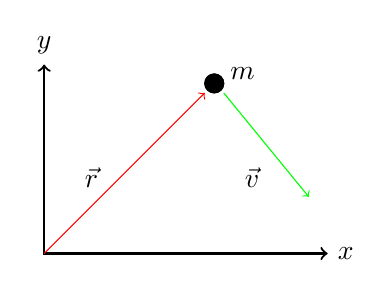
\begin{tikzpicture}[scale=1.2]
\draw [<->,thick] (0,2) node (yaxis) [above] {$y$}
        |- (3,0) node (xaxis) [right] {$x$};
\draw[->, red](0,0)--(1.7,1.7);
\filldraw[fill=black] (1.8,1.8) circle (0.1);
\draw (2.1,1.9) node (mass) {$m$};
\draw (.5,.8) node{$\vec{r}$};
\draw [fill=black] (1.8,1.8) circle(0.1);
\draw[->, green](1.9,1.7)--(2.8,0.6);
\draw (2.2,.8) node{$\vec{v}$};
\end{tikzpicture}
\end{marginfigure}


\bas
    \rmt{Linear Momentum: } & \vec{P} = m\vec{v}\\
    \rmt{Angular Momentum: } & \vec{L} =\vec{r}\times\vec{p}\\
    \rmt{Kinetic Energy: } & T  = \frac{1}{2}m v^2 = \frac{\abs{\vec{P}}^2}{2m}\\
    \rmt{Total Mechanical Energy: } & H  = T + V
\eas

The quantities, together with the position of the object, describe the classical \emph{state} of the system. The conservation laws corresponding to these quantities are also useful.
\marginnote[-2cm]{All three of these conservation laws are closely connected to symmetries, thanks to Noether's Theorem.  Conservation of Linear Momentum corresponds to a translational symmetry, Angular momentum corresponds to rotational symmetry, and conservation of energy corresponds to time translational symmetry.}
\bas
    \rmt{Conservation of Linear Momentum: } & \rmt{If } \sum{\vec{F}_\rmt{ext}}=0  \rmt{, then } \frac{d\vec{P}}{dt}=0\\
    \rmt{Conservation of Angular Momentum: } & \rmt{If } \sum{\vec{\tau}_\rmt{ext}}=0  \rmt{, then }\frac{d\vec{L}}{dt}=0\\
    \rmt{Conservation of Mechanical Energy: } & \rmt{If } \frac{\partial V}{\partial t}=0 \rmt{, then } \frac{dH}{dt}=0
\eas

\section{Electricity and Magnetism}

We will often be dealing with charged particles in our quantum systems, so it will be useful to have a handful of relationships from E\&M available to us.  First, we've got the basic electric field $\vec{E}$ at a position $\vec{r}$ due to a point charge $q_1$, which is:
\begin{marginfigure}[-1cm]
\centering
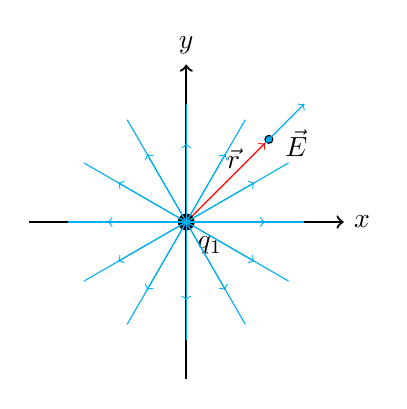
\begin{tikzpicture}[scale=1]
\draw [->,thick] (0,-2) -- (0,2) node (yaxis) [above] {$y$};
\draw [->,thick] (-2,0) -- (2,0) node (xaxis) [right] {$x$};

\draw (.3,-.3) node (charge) {$q_1$};
\draw (.6,.8) node{$\vec{r}$};
\draw[->,red](0,0) -- (1,1);
\filldraw[fill=black] (0,0) circle (0.1);

\filldraw[fill=cyan] (1.05,1.05) circle(0.05);
\draw[->,cyan](1,1)--(1.5,1.5);
\draw (1.4,1) node{$\vec{E}$};

\foreach \a in {0, 30,...,359}
    \draw[thin,cyan] (\a:0) -- (\a:1.5); 
\foreach \a in {0, 30,...,359}
    \draw[thin,cyan,->] (\a:0) -- (\a:1); 
    
\end{tikzpicture}
\end{marginfigure}
\beq
\vec{E} = \frac{1}{4\pi\epsilon_0}\frac{q_1}{r^2}\hat{r}.
\label{eq:efield}
\eeq

Then if we place a second charge $q_2$ near the first charge, we can find the electric potential energy $V$:
\begin{marginfigure}[-1cm]
\centering
\begin{tikzpicture}[scale=1.2]
\draw [<->,thick] (0,2) node (vaxis) [above] {$V$}
        |- (3,0) node (xaxis) [right] {$r$};
\draw[color=blue,domain=0.5:3] plot (\x,{1/(\x)}) node[right] {$V = \frac{1}{4\pi\epsilon_0}\frac{q_1q_2}{r}$};
\end{tikzpicture}
\end{marginfigure}

\beq
V = \frac{1}{4\pi\epsilon_0}\frac{q_1 q_2}{r}.
\eeq

We'll be using the dipole model for a number of different systems.  An electric dipole $\vec{p}_E$ is created when two charges of equal magnitude and opposite charge are separated by a distance $\vec{d}$,
\begin{marginfigure}
\centering
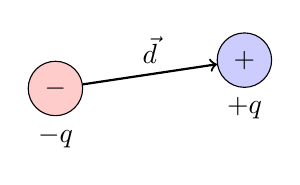
\begin{tikzpicture}[scale=1.2]
\path ( 0,0) node (q1) [shape=circle,draw,fill=red!20,label=below:$-q$] {$-$}
 ( 2,.3) node (q2) [shape=circle,draw,fill=blue!20,label=below:$+q$] {$+$};
 \draw [->,thick] (q1) -- (q2) node[above,midway]{$\vec{d}$};
\end{tikzpicture}
\end{marginfigure}
\beq
\vec{p}_E = q \vec{d}.
\eeq

Similarly, we can define the magnetic dipole $\vec{\mu}$ that is created when a current $I$ flows around a circle of area $A$ with normal vector $\hat{n}$,
\begin{marginfigure}
\centering
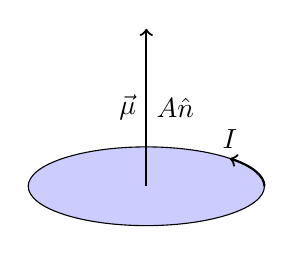
\begin{tikzpicture}[scale=1]
 \draw [fill=blue!20] (0,0) ellipse (1.5 and 0.5);
 \draw [->,thick] (0,0) -- (0,2) node[right,midway]{$A\hat{n}$} node[left,midway]{$\vec{\mu}$};
 \draw [->, thick] (1.5,0) arc (0:45:1.5 and 0.5) node[above]{$I$};
\end{tikzpicture}
\end{marginfigure}
\beq
\vec{\mu} = I A \hat{n}.
\eeq

When the magnetic dipole $\vec{\mu}$ is in an external magnetic field $\vec{B}$, there is a potential energy due to the interaction between the dipole and the field:
\begin{marginfigure}
\centering
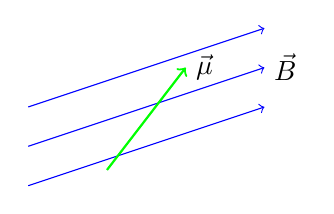
\begin{tikzpicture}[scale=1]
\draw[->,blue] (0,0) -- (3,1);
\draw[->,blue] (0,0.5) -- (3,1.5) node[right,black]{$\vec{B}$};
\draw[->,blue] (0,1) -- (3,2);
\draw[->,green,thick] (1,0.2) -- (2,1.5) node[right,black]{$\vec{\mu}$};

\end{tikzpicture}
\end{marginfigure}
\beq
V_\textrm{dip}= - \vec{\mu}\cdot\vec{B}.
\eeq

\begin{example}
\label{ex:orbitalmu}
What is the magetic moment for a single electron ``orbiting'' a single proton at the Bohr radius $a_0=(4\pi\epsilon_0\hbar^2)/(m_e e^2)$?

\model We'll model both the electron and the proton as point charges and point masses. We'll also model the electron as undergoing uniform circular motion without any losses (friction, radiation, etc.).

\vis We picture this as a circular orbit shown in Figure \ref{fig:exorbit}.
\begin{figure}
\centering
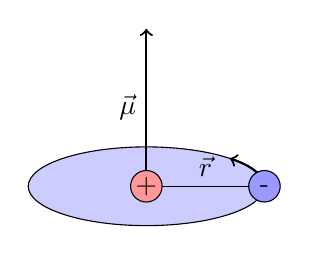
\begin{tikzpicture}
 \draw [fill=blue!20] (0,0) ellipse (1.5 and 0.5);
 \draw [->,thick] (0,0) -- (0,2) node[left,midway]{$\vec{\mu}$};
 
 \draw [->, thick] (1.5,0) arc (0:45:1.5 and 0.5);
 \draw (0,0) -- (1.5,0) node[midway,above] {$\vec{r}$};
 \draw[fill=blue!40] (1.5,0) circle (.2) node{-};
 \draw[fill=red!40] (0,0) circle (.2) node{+};
 
\end{tikzpicture}
\caption[][2cm]{ Circular electron ``orbit''.}
\label{fig:exorbit}
\end{figure}

\sol Since the distance between the proton and the electron stays constant, the area swept out by the electron is: $A = \pi a_0^2$. Since we are modeling the electron as going in uniform circular motion with a period $T$, the current is just $I = e/T$. We can use the uniform circular motion model along with the Coulomb force ($F = m_e v^2/a_0= eE$) to find the period of the motion, since, for uniform circular motion, the velocity is $v = (2\pi a_0)/T$. This means that 
\beq
\frac{e}{T}=\sqrt{\frac{1}{4\pi\epsilon_0}\frac{e^2}{a_0^2}\frac{e^2}{4\pi^2a_0m_e}}.
\eeq
So, the magnetic dipole moment is:
\beq
\mu=I A = \pi a_0^2 \frac{e}{T} = \frac{e \hbar}{2m_e}.
\eeq\arnote[-1.5cm]{Work through this to make sure you get the end step.}
Of course, you should run through this algebra in your notes and make sure you get the same answer. I mean it --- stop right now and do it!

\assess Checking our units, we expect to have units [m$^2$ C/s]. What we got has units: [C J$\cdot$s/kg] which is [C (kg$\cdot$m$^2$/s)/kg] which is what we want.

\end{example}


\begin{exercise}
What would the stored potential energy (in eV) of a charged system be if we held a single proton and a single electron apart the distance of the classical Bohr radius?

\end{exercise}


\section{Electromagnetic Waves}
\label{sec:elmaw1}
Of course we are going to need some mechanisms to describe the behavior of light. We'll start with a straight-forward description of a plain electromagnetic wave propagating along the $x$ axis.\marginnote{We use the term {\em electromagnetic wave} so much, we'll shorten it to {\em ElMaW}, pronounced like ``elmer'' with a softer end.} The wavelength is $\lambda$ and we define the wavenumber $k=2\pi/\lambda$.  Similarly, the wave has a time period of $T$ and an angular frequency $\omega = 2\pi/T$.  In this configuration we have coupled electric and magnetic fields:
\begin{marginfigure}
\centering
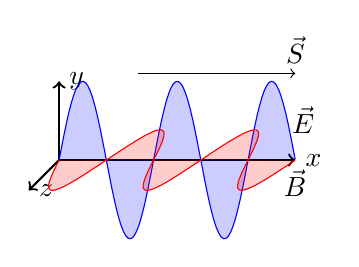
\begin{tikzpicture}[scale=1]
\draw[->,thick] (0,0,0) -- (3,0,0) node[right]{$x$};
\draw[->,thick] (0,0,0) -- (0,1,0) node[right]{$y$};
\draw[->,thick] (0,0,0) -- (0,0,1) node[right]{$z$};
\draw[color=blue,domain=0:3,fill=blue,samples=100, fill opacity=0.2] plot (\x,{sin(300*\x)},0) node[right,above,black,fill opacity=1,shift={(.1,.2,0)}] {$\vec{E}$};
\draw[color=red,domain=0:3,fill=red,samples=100, fill opacity=0.2] plot (\x,0,{sin(300*\x)}) node[right,below,black,fill opacity=1] {$\vec{B}$};
\draw[->](1,1.1,0) -- (3,1.1,0) node[above]{$\vec{S}$};
\end{tikzpicture}
\end{marginfigure}
\bas
E_y =& E_0 \sin(kx - \omega t)\\
B_z =& B_0 \sin(kx - \omega t).
\eas
For an electromagnetic wave moving through vacuum, the electric field and magnetic field amplitudes are related to each other such that $B_0 = E_0/c$, where $c$ is the speed of light, which, in turn, is also related to the electric field and magnetic field constants $\epsilon_0$ and $\mu_0$:
\beq
c^2 = \frac{1}{\mu_0\epsilon_0}.
\eeq
We need a couple of more things about electromagnetic waves. First, the Poynting vector $\vec{S}$ describes the movement of energy of the electromagnetic wave and can be written in terms of the electric and magnetic fields, pointing in the direction of propagation:
\beq
\vec{S}=\frac{1}{\mu_0}\vec{E}\times\vec{B} =c\epsilon_0 E_0^2 \hat{x} \sin^2(kx - \omega t).
\label{eq:poynting}
\eeq
We can now relate the energy transmission of the electromagnetic wave (per unit area) to the Poynting vector: 
\beq
I =\abs{\vec{S}_\rmt{avg}} = \frac{c\epsilon_0}{2}E_0^2.
\eeq

\begin{marginfigure}
\centering
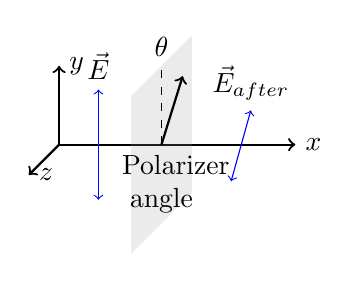
\begin{tikzpicture}[scale=1]
\draw[->,thick] (0,0,0) -- (3,0,0) node[right]{$x$};
\draw[->,thick] (0,0,0) -- (0,1,0) node[right]{$y$};
\draw[->,thick] (0,0,0) -- (0,0,1) node[right]{$z$};
\draw[color=blue,<->](.5,-.7,0) -- (.5,.7,0) node[above,black]{$\vec{E}$};
\fill[fill=black!40, fill opacity=0.2] (1.3,-1,-1)--(1.3,-1,1)--(1.3,1,1)--(1.3,1,-1)--cycle;
\draw[dashed](1.3,0,0) -- (1.3,1,0) node[above]{$\theta$};
\draw[->,thick](1.3,0,0) node[below,text width=1cm,align=center]{Polarizer angle}-- (1.3,.6,-.7) ;
\draw[color=blue,<->](2.3,-.35,.3) -- (2.3,.3,-.35) node[above,black]{$\vec{E}_\rmt{after}$};
\end{tikzpicture}
\end{marginfigure}
And, finally, we need to say something about the polarization of the wave. Because we are typically going to be working with a model that the interaction between the electromagnetic waves and matter will be dominated by the electric field, we define the polarization as the direction of the electric field vector. The effect of passing through a polarizer is to only pass the component of the electric field vector that points along the direction of the polarizer \ie $E_\rmt{final} = E_\rmt{initial} \cos\theta$, where $\theta$ is the angle between the polarizer and the incoming electric field vector. If we send randomly polarized light, the polarizer will pass half the initial intensity  and the output electric field will be polarized along the polarizer direction.

\begin{exercise}
A beam of unpolarized light from the sun with an initial intensity of 1000 W/m$^2$ passes through an initial polarizer, then through a second polarizer rotated by 45$^\circ$. What is the intensity and polarization of the output beam?
\end{exercise}


\subsection{Field Superposition}
We will frequently use the concept of superposition. The idea is that if we have two waves (or two electric fields, or two magnetic fields, etc.), we can find the total amplitude by adding up the amplitudes of the combined waves (or fields). In terms of the electric field, this means that the net (or total) electric field $\vec{E}_\rmt{total}$ at a point is a sum of all $N$ electric fields at that point:
\beq
\vec{E}_\rmt{total} = \sum_{i=1}^{N}\vec{E}_i
\eeq

\section{Waves}
\label{sec:waves}
A function that is propagating with some speed $v$ can be written in general as a right-moving wave (in the positive $x$ direction): $f(x - vt)$, or as a left-moving wave $f(x+vt)$. We saw this in the electromagnetic waves above for a sine wave, but it works in general for any function.

If we have two waves with the same amplitude along the same axis, but moving in opposite directions, it is the same as having a standing wave, i.e. a wave that oscillates up and down but does not move left or right.
\begin{example} What is the net wave if two traveling beams of light going opposite directions interfere in a region of space?

\model We model the two beams as electromagnetic waves with the same wavelength and frequency as the oscillations of their electric fields. 

\vis We have two waves approaching each other in Figure \ref{fig:wavesexample}.

\begin{figure}
\centering
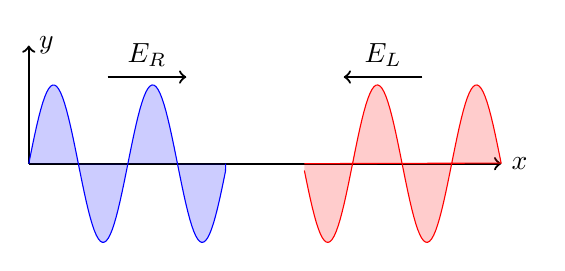
\begin{tikzpicture}
\draw[->,thick] (0,0) -- (6,0) node[right]{$x$};
\draw[->,thick] (0,0) -- (0,1.5) node[right]{$y$};
\draw[color=blue,domain=0:2.5,fill=blue,samples=100, fill opacity=0.2] (0,0) plot (\x,{sin(286*\x)}) -- (2.5,0)  ;
\draw[color=red,domain=3.5:6,fill=red,samples=100, fill opacity=0.2] (6,0) plot (\x,{sin(286*(6-\x)}) -- (3.5,0);
\draw[->,thick] (1,1.1) -- (2,1.1)node[midway,above,black,fill opacity=1] {$E_\rmt{R}$};
\draw[->,thick] (5,1.1) -- (4,1.1)node[midway,above,black,fill opacity=1] {$E_\rmt{L}$};
\end{tikzpicture}
\caption[][2cm]{ }
\label{fig:wavesexample}
\end{figure}

\sol Both waves are moving, one to the right and one to the left
\beq
E_\rmt{R}=E_0\cos(kx - \omega t)\ \rmt{and}\ E_\rmt{L}= E_0\cos(kx + \omega t)
\eeq
We find the sum of the two waves by applying the superposition principle: $E_\rmt{total}=E_\rmt{R}+E_\rmt{L}$. When we add these two waves, we re-write the trig functions such that we get a total wave amplitude of:
\beq
E_\rmt{total}=2E_0\cos kx \cos \omega t
\eeq
which is a standing wave as we expected. Of course, like usual, you need to go work out that trig work on your own.

\assess The maximum amplitude we get with this superposition is $2E_0$, which makes sense. The best way to assess this, though, is to animate it using your \CAS~and make sure it does what you want it to do. 

\end{example}
\arnote[-6cm]{Work through this to make sure you get the end step. Here's a hint: use a \texttt{TrigExpand} function on your favorite computer algebra system (\CAS) to get things rolling.}

\subsection{General Interference}
We can work with the superposition of any two waves by looking at the way in which the phases of the waves interact. We consider two electric field waves $E_1$ and $E_2$ that have the same wavelength and frequency but have a different phase offset $\phi_1$ and $\phi_2$:
\bas
E_1=&E_0\cos(kx-\omega t + \phi_1)\\
E_2=&E_0\cos(\underbrace{kx-\omega t + \phi_2}_{\rmt{Total wave phase}}).
\eas
We typically are looking for places where the waves add constructively or destructively. We will find constructive inference if the total phase of the sum of the waves $\Delta\phi$ is an integer multiple of $2\pi$. The interference will be destructive if the total phase is a half-integer multiple of $\pi$:
\beq 
\left.
\begin{aligned}
\rmt{Constructive: } & \Delta\phi = 2\pi n\\
\rmt{Destructive: } & \Delta\phi = 2\pi \left(n+\frac{1}{2}\right)
\end{aligned}
\right\}\  n=0,1,2,\ldots
\eeq
In one dimension, we model the total phase difference as the difference between the wave positions $\Delta x$ plus any initial phase offset $\Delta \phi$:
\arnote{Work through this to make sure you get the end step.}
\bas
\Delta\phi = & (kx_2 - \omega t + \phi_2) - (kx_1 - \omega t + \phi_1)\\
= & k\Delta x + \Delta\phi_\rmt{init}
\eas
where $\Delta x= x_2 - x_1$ and  $\Delta\phi_\rmt{init} = \phi_2-\phi_1$.

\subsection{Math Interlude: Complex Numbers}
We will be using complex numbers extensively. A complex number $z$ (and its complex conjugate $z^*$) can be written in terms of real numbers $x$, $y$, $r$, and $\theta$ in a number of different ways:
\bas
z &=x+\I y         & z^*&=x-\I y         & x &=r \cos\theta\\
 &=r\E{\I\theta} & &=r\E{-\I\theta}   & y &=r \sin\theta.
\eas

\section{Complex Electromagnetic Wave Amplitude Model (CEWAM)}
\label{sec:CEWAM}
It is really useful to model the electromagnetic waves using complex numbers. This will make it much easier for us to do calculations in a number of situations. The model (in one dimension) describes a traveling wave polarized in the $y$-direction as
\beq
E_y = E_0\E{\I(kx-\omega t)}.
\label{eq:CEWAM}
\eeq
When we want to connect back to the real electric field, we expand the exponential using the Euler formula and then take the real part.\marginnote{The Euler formula is:
\beq\E{\I\theta} = \cos\theta + \I\sin\theta.\eeq} The intensity of this wave is then calculated by taking the electric field times its complex conjugate:
\beq
I = \frac{c \epsilon_0}{2}E E^* = \frac{c \epsilon_0}{2}\abs{E}^2 = \frac{c \epsilon_0}{2}E_0^2,
\label{eq:CEWAMInt}
\eeq
where we have used the notation $EE^*$ = $\abs{E}^2$. Also note that when you multiply a complex number by its complex conjugate, the phase pieces multiply to give $1$: $\E{\I\theta}\E{-\I\theta}=\E{0}=1$.

\arnote[10cm]{As usual, work through this to make sure you get the end step. Look up the trig identities and how they relate to the complex exponential. Try using \texttt{ExpToTrig} with your favorite \CAS. }

\begin{example}
Use the CEWAM to find the interference intensity of two light beams that are slightly offset in one dimension.

\model We will model the two electromagnetic waves as moving in the same direction with the same frequency, wavelength and amplitude (which will stay constant) using the complex amplitude model. We'll model the beam offset as a $\Delta x$.

\vis The two waves are offset by just a bit, shown in Figure \ref{fig:excewam2}.

\begin{figure}
\centering
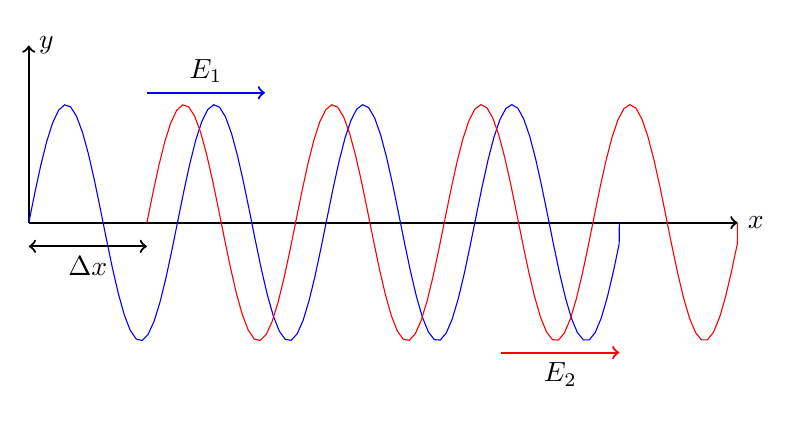
\begin{tikzpicture}[scale=1.5]
\draw[->,thick] (0,0) -- (6,0) node[right]{$x$};
\draw[->,thick] (0,0) -- (0,1.5) node[right]{$y$};
\draw[color=blue,domain=0:5,samples=100] (0,0) plot (\x,{sin(286*\x)}) -- (5,0)  ;
\draw[color=red,domain=1:6,samples=100] (1,0) plot (\x,{sin(286*(\x-1)}) -- (6,0);
\draw[->,thick,blue] (1,1.1) -- (2,1.1)node[midway,above,black,fill opacity=1] {$E_1$};
\draw[->,thick,red] (4,-1.1) -- (5,-1.1)node[midway,below,black,fill opacity=1] {$E_2$};
\draw[<->,thick](0,-.2) -- (1,-.2) node[midway,below]{$\Delta x$};
\end{tikzpicture}
\caption[][2cm]{ }
\label{fig:excewam2}
\end{figure}

\sol Since we are interested in the intensity (the one thing we can easily measure), we need to find the net electric field amplitude and then use Eq.~(\ref{eq:CEWAMInt}) to find the intensity of the combined beams.
\bas
E_1 &=  E_0 \E{\I(k x_1 -\omega t)}\\
E_2 &=  E_0 \E{\I(k x_2 -\omega t)}.
\eas
The net electric field is then $E_\rmt{total} =E_1 + E_2$. We just add these together and then find the intensity:
\bas
I=& \frac{c \epsilon_0}{2}E_\rmt{total} E_\rmt{total}^*\\
=&\frac{c \epsilon_0}{2}\left(\abs{E_1}^2+\abs{E_2}^2 + E_1^*E_2 + E_1 E_2^*\right)\\
=&\frac{c \epsilon_0}{2}\left(2E_0^2 + E_0^2\left(\E{\I(k x_2-k x_1)}\right) + E_0^2\left(\E{\I(k x_1-k x_2)}\right)\right)\\
=&\frac{c \epsilon_0}{2}E_0^2\left(2 + 2 \cos(k\Delta x) \right).
\eas
So the intensity could be anywhere from a maximum of $2c\epsilon_0 E_0^2$ if $k\Delta x = 0, 2\pi, 4\pi, \ldots$ to a minimum of zero if $k \Delta x = \pi, 3\pi, \ldots$. 

\assess The limits look right for the max and the min: a max happens when $\Delta x = 2 \pi/k = \lambda$, which makes sense. The minima happened when $\Delta x = \lambda/2$.

\end{example}

\begin{exercise}
Use the CEWAM to find the interference of two point-source waves (i.e. the double-slit interference model) on a screen a long distance away from the sources. I encourage you to go back to your notes from previous classes to see how you did this before and then do it again with this new model.
\end{exercise}

\begin{exercise}
Describe the motion and behavior of a polarized wave with the following components:
\bas
E_y =& E_0 \E{\I(kx -\omega t)}\\
E_z =& E_0 \E{\I(kx -\omega t + \pi/2)}.\\
\eas

\end{exercise}

%----------------------------------------------------------------------------------------
% Chapter 2
%----------------------------------------------------------------------------------------
\chapter{Creating Electromagnetic Waves}

Ok, this really is a guidebook for a quantum mechanic. And we really will get to doing some work under the hood, so to speak, with our quantum tools. However, I want to motivate the need for a new set of models to describe the quantum world. So we look for places or situations where our current models don't seem to work any more. One of those is in the uniform circular motion model of the electron orbiting around the proton. We've used the model a number of times, but there is a real problem with it. To get at that problem, we need to build of model of electromagnetic wave generation.

\section{Classically Accelerated Charges}
We introduced, back in introductory physics, the idea that an accelerating charge can generate an electromagnetic wave. We used a simple model where we have an oscillating current moving up and down a long center-fed wire.
\begin{marginfigure}\centering
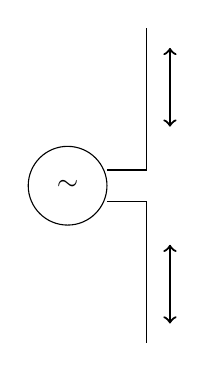
\begin{tikzpicture}[scale=1]
\draw (0,0) circle (.5) node(source){$\sim$};
\draw(.5,.2) -- (1,.2) -- (1,2);
\draw(.5,-.2) -- (1,-.2) -- (1,-2);
\draw[<->,thick](1.3,.75) -- (1.3,1.75);
\draw[<->,thick](1.3,-.75) -- (1.3,-1.75);
\end{tikzpicture}
\end{marginfigure}

As the electrons accelerate up and down, the electric and magnetic fields they produce begin to look like electromagnetic waves. We will build a simple model for how an accelerating electric charge can generate electromagnetic waves.
\subsection{Larmor Radiation}
\marginnote{We're following Purcell's derivation here.}
Here's the model: a single electron is traveling at a constant speed $v$. After some time $T$, the electron abruptly decelerates to rest (for a total change in velocity of $\Delta v$) over a short time interval $\Delta T$. If we look at the electric field lines that could come from the charge, we would get something that looks like the figure on the right. However, the electric field lines must have smoothly shifted from the one position to the other, so we will focus in on how they make that transition.

\begin{marginfigure}\centering
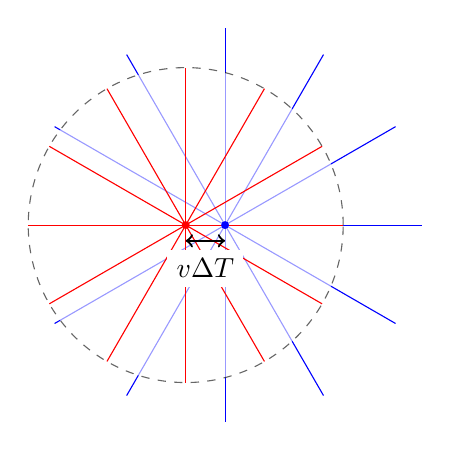
\begin{tikzpicture}[scale=1]
  \begin{scope}[shift={(0.5,0)}]
    \foreach \a in {0, 30,...,359}
    \draw [blue](\a:0) -- (\a:2.5); 
  \end{scope}
\filldraw[dashed, fill=white, opacity=0.6] (0,0) circle (2);
\foreach \a in {0, 30,...,359}
    \draw [red] (\a:0) -- (\a:2); 
\draw[<->,thick] (0,-.2) -- (0.5,-.2) node[fill=white,below,midway,shift={(0,-.1)}]{$v \Delta T$};
\fill[red] (0,0)circle(0.05);
\fill[blue] (.5,0) circle(0.05);
\end{tikzpicture}
\end{marginfigure}

Zooming in on one line, we have the following, where we have expanded the short deceleration interval $\Delta T$ which is much faster than the time $T$.  The blue point is where the charge {\em would have been} if it hadn't stopped. In particular, we are interested in the radial and transverse components of the electric field $E_r$ and $E_t$ during the acceleration interval. We assume that the signal of the acceleration travels outward at the speed of light. At some time $T$ later, the signal has traveled $r=cT$ as depicted in Figure \ref{fig:larmor}.

\begin{figure}
\centering
\begin{tikzpicture}[scale=2]

\fill[fill=blue!20] (2,0) -- (2.5,0) arc(0:60:2.5) -- (60:2) -- (60:2) arc(60:0:2);
\draw[dashed] (2,0) arc (0:60:2);
\draw[dashed] (2.5,0) arc (0:60:2.5);
\draw[<->] (50:2) -- (50:2.5) node[above,shift={(.4,0)}]{$c\Delta T$};
\draw[<->,thick] (-.5,-.2) -- (0,-.2) node[below,midway,shift={(0,-.1)}]{$v T$};
\fill[blue] (0,0)circle(0.05);
\fill[red] (-.5,0) circle(0.05);
\begin{scope}[shift={(-0.5,0)}]
    \draw[thick](30:0) coordinate(pt4) -- (30:2.43) coordinate(pt2) node[midway,above,shift={(-.5,0)}]{$r=cT$};
\end{scope}

\draw[thick] (-1,0) -- (3,0);
\draw[dashed](1,0) arc (0:30:1) node[midway,right]{$\theta$};

\draw[dashed] (30:0) coordinate(pt0) -- (30:2.5) coordinate(pt1);
\draw[thick] (pt2) -- (pt1);
\draw[thick] (30:2.5) -- (30:2.95);
\draw[<->,red] (30:2) coordinate(pt3) -- (30:2.5) node[midway,below]{$E_r$};
\draw[<->,red] (pt2)--(pt3) node[midway,left,shift={(0,-0.2)}]{$E_t$};
\draw[dashed] ($(pt4)!(pt0)!(pt2)$) -- (pt0) node[midway,right,rotate=30] {$v T \sin\theta$};
\end{tikzpicture}
\caption[][2cm]{The electric field lines are offset by the accelerated charge.}
\label{fig:larmor}
\end{figure}

We now look at the ratio of the two electric field components $E_t/E_r$ which is unitless:
\beq
\frac{E_t}{E_r} = \frac{v T \sin\theta}{c\Delta T}.
\eeq

But the radial electric field in just given by Eq.~(\ref{eq:efield}), so we have:
\beq
E_t = \frac{q}{4\pi\epsilon_0 r^2} \frac{(v/\Delta T) (cT)}{c^2}\sin\theta.
\label{eq:etprelarmor}
\eeq
Since $v/\Delta T$ is the acceleration $\dot{v}$ and the radius $r = cT$, we simplify this to:
\arnote{Make sure you can get here in your notes.}
\beq
E_t = \frac{q}{4\pi\epsilon_0 r^2} \frac{\dot{v}r}{c^2}\sin\theta.
\eeq
The outgoing energy transmission per unit area of this transverse electric field is given by the Poynting vector, Eq.~(\ref{eq:poynting}), $S =c\epsilon_0E_t^2$. This means that the total energy loss $dU/dt$ must be integrated over the whole sphere of radius $r$:
\beq
\frac{dU}{dt} = \int_{0}^{2\pi}\int_{0}^{\pi} S\ r^2 \sin\theta d\theta d\phi.
\label{eq:dudtprelarmor}
\eeq
Use your favorite \CAS to do this integral and you should get the rate of energy loss by an accelerating charge as:
\beq
\frac{dU}{dt} = \frac{q^2\dot{v}^2}{6\pi c^3\epsilon_0}
\label{eq:larmor}
\eeq\marginnote[-1.5cm]{You will work this out as an exercise.}
which is known as the Larmor radiation formula.
\begin{exercise}
Work through the steps needed to get from Eq.~(\ref{eq:etprelarmor}) to Eq.~(\ref{eq:larmor}). Be sure to include your model, visualization, and assessment (\ie check that the units work out).
\end{exercise}



\section{Hydrogen Radiation Problem}
We now have everything we need to re-visit the model of an electron in uniform circular motion about a stationary proton. The radial acceleration (from $F_r = m a_r$) of the electron is
\begin{marginfigure}\centering
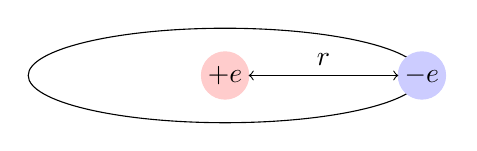
\begin{tikzpicture}[scale=1]
\draw (0,0) ellipse(2.5 and .6);

\filldraw[red!20] (0,0)circle(0.3) node[black]{$+e$};
\filldraw[blue!20] (2.5,0) circle(0.3) node[black]{$-e$};
\draw[<->](.3,0) -- (2.2,0)node[above,midway]{$r$};

\end{tikzpicture}
\end{marginfigure}
\beq
a_r = \dot{v} = \frac{1}{m_e}\frac{e^2}{4\pi\epsilon_0r^2}.
\eeq

We'll model the electron as it orbits the proton at a distance of $a_0$, the Bohr radius we used in Example \ref{ex:orbitalmu}. But, as we just saw with the Larmor formula, any charged particle undergoing accelerations emits radiation. The energy emitted must come from somewhere --- and in this case, it must be from the mechanical energy of the orbit. We need the total mechanical energy for an object undergoing uniform circular motion. We know the potential and kinetic energies. We use the fact that we are going in circular motion to simplify the total energy to $U = -e^2/(4\pi\epsilon_0 (2r))$. \arnote{There are a bunch of steps I skipped in here. Go through them and be explicit on each step so that you get this same result.} We take the time derivative of this to get
\beq
\frac{dU}{dt}=\frac{e^2}{4\pi\epsilon_0}\frac{\dot{r}}{2r^2}.
\label{eq:energyderivative}
\eeq
We want how the radius changes with time (with an initial radius of $a_0$). So we equate this with Eq.~(\ref{eq:larmor}) to get a differential equation: \arnote{I skipped steps here, too. Work through them on your own.}
\beq
\dot{r}r^2 = -\frac{e^4}{12\pi^2\epsilon_0^2 c^3 m_e^2}.
\label{eq:rrdot}
\eeq
It helps some if we define a new length scale: $r_e = e^2/(4\pi\epsilon_0 c^2 m_e)$. We can then write the differential equation as:
\beq
\dot{r}r^2=-\frac{4}{3}r_e^2 c,
\eeq
which has a straight-forward solution with the initial condition that $r=a_0$ at $t=0$: \arnote{Three in a row-- work these out, too.}
\beq
r^3 = a_0^3-4 r_e^2 c t.
\label{eq:orbitdecay}
\eeq

Here's the problem with this model: Eq.~(\ref{eq:orbitdecay}) predicts that the orbit of the electron will start at $a_0$ and quickly decay to zero as seen in the figure! Furthermore, we don't measure this type of radiation coming from the hydrogen atom. So this model doesn't work. Similarly, no model where the electron is moving in any kind of classical orbit around the proton will work - they will all have this same problem. So we need a new model where the electron stays bound to the proton, but not in a classical orbit. \begin{marginfigure}\centering
\begin{tikzpicture}[scale=1]
\draw[->,thick] (0,0) node[left]{0} -- (4,0) node[right]{$t$};
\draw[->,thick] (0,0) node[below]{0}-- (0,3) node[right]{$r$};
\draw[color=blue,domain=0:3,samples=100] plot (\x,{(2^3-(2^3/3)*\x)^(1/3)});
\draw (0,2) node[left]{$a_0$};
\end{tikzpicture}
\end{marginfigure}

\section{Bohr Model}
\label{sec:bohr}
We have another piece of data that also points to the need for a new model. If the electron could classically orbit the proton, it should be able to orbit it at any radius. As the electron moved from one radius (total mechanical energy) to another (new total energy), there should be some kind of energy absorption or emission corresponding to this change in internal energy. If the electron can occupy any orbit, we would expect a continuous spectrum of energy emission. We measure energy emission from the hydrogen atom, but it isn't continuous.
\begin{marginfigure}\centering
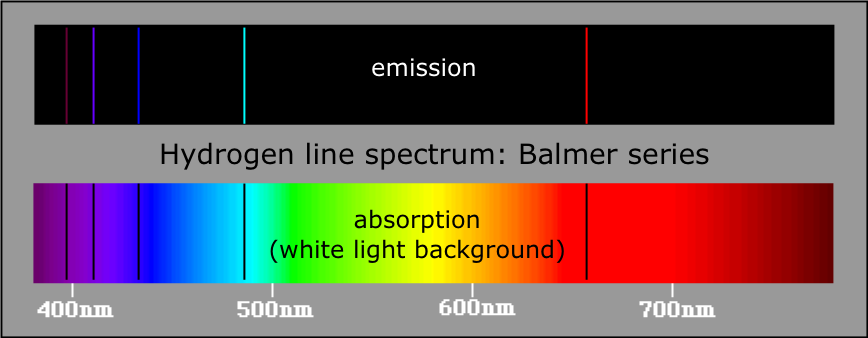
\includegraphics[width=\textwidth]{Balmer.png}
\caption{From \href{http://chemwiki.ucdavis.edu/Textbook_Maps/General_Chemistry_Textbook_Maps/Map\%3A_Lower's_Chem1/04._Atoms_and_the_Periodic_Table/The_Bohr_Atom}{\texttt{chemwiki.ucdavis.edu/
Textbook\_Maps/General\_Chemistry
\_Textbook\_Maps/Map\%3A\_Lower's
\_Chem1/04.\_Atoms\_and\_the
\_Periodic\_Table/The\_Bohr\_Atom}}
}
\end{marginfigure}
There is a pattern to the emission lines if we make two assumptions: first, that the electron can only exist in specific energy configurations. We won't say anything more specific about these yet, but we can empirically note that the energy associated with each of the configurations is
\beq
E_n = -\frac{R_\infty h c}{n^2}
\eeq
where $R_\infty$ is a constant with units 1/length, $c$ is the speed of light, $h$ is Planck's constant, and $n$ is a positive integer. The second assumption is that the energy associated with the emitted light is inversely proportional to its wavelength with constant of proportionality $hc$ (where $c$ is the speed of light and $h$ is Planck's constant):
\beq
E = \frac{h c}{\lambda}.
\eeq
Put those two together and we see that the emitted wavelengths as the electron jumps from one configuration to another (like from $n_1$ to $n_2$) is
\beq
\frac{1}{\lambda} = \abs{R_\infty\left(\frac{1}{n_2^2} -\frac{1}{n_1^2}\right)}.
\eeq\marginnote{The \href{http://physics.nist.gov/cgi-bin/cuu/Value?ryd|search_for=rydberg}{numerical value of $R_\infty$} is $10973731.6$~m$^{-1}$.}%
Of course, there is more to this than the simple empirical relationship. However, this is enough for us for now. Each time the electron in an atom jumps from one allowed energy configuration to another it either absorbs energy from an electromagnetic wave (if it increases energy) or emits an electromagnetic wave (if it decreases in energy).

\begin{exercise}
\begin{enumerate}
\item There are a couple of named sequences of emission lines from the hydrogen atom. The second of these is the Balmer series which ends at a final energy configuration where $n_f = 2$. Calculate the first 6 possible wavelengths of transitions from higher energy states to this final state, plus the energy to go from $n=\infty$ to this state. Show your work (I don't really care if you can look up the answer on the internet. If I really needed you to give me the answer, I'd have done it myself. The point is to give you practice doing calculations!)

\item Do the same thing for the Bohr series where $n_f = 3$. Calculate the first 6 possible wavelengths of transitions from higher energy states to this final state, plus the energy to go from $n=\infty$ to this state. Show your work.
\end{enumerate}
\end{exercise}

\section{Detecting Electromagnetic Waves}

The last thing we need to do to get to a place where we explore quantum states is to build a model for detecting electromagnetic waves. We're almost there. Let's review what we know about electromagnetic waves (ElMaWs) and how we could detect them.

\begin{enumerate}
\item ElMaWs can make charges in matter accelerate. If we could connect a very fast ammeter to some kind of metal antenna, we could detect the wave. That works well for radio waves, but by the time we get to the visible wavelengths, the wave oscillations are too fast to measure.
\item ElMaWs carry energy. The intensity of a wave is a measure of power/area which is energy/(time$\cdot$area). So the energy deposited by an ElMaW could be detected and used.
\item We could measure the change in temperature as the energy from the ElMaW deposits its energy in a material. This works well, but tends to be slow - materials take time to heat up and respond thermally.
\item What if the incomming ElMaW has a wavelength less than $1/R_\infty$? Following our model from the last chapter, this corresponds to a transition going from $n=1$ to $n=\infty$. What does that mean? Experimentally, it means that the electron has climbed out of the potential well and is no longer bound to the proton - it has become a free electron! All we have to do now is detect that electron and we're home free!
\item The incoming ElMaW could cause a chemical change in a molecule. We could use chemistry to isolate the molecules that have undergone the chemical change and thus detect where the ElMaW was. This is how photopaper works.
\item Finally, we could use a semiconductor where there is an energy gap between an insulator state and a conductor state. If the incoming ElMaW has more energy than the size of the gap, it can deposit its energy, creating a current. We can then detect that current using an ammeter. This is how photovoltaics work.

\end{enumerate}

\subsection{Electron Detection}

There are a couple of ways we can detect a single free electron. One way is to use a series of positively charged plates to amplify the electron signal to a point where it can be detected. This is basically the way a photomultiplier works (PMT).  A microchannel plate (MCP) works in about the same way. So we have the tools we need to detect single free electrons, though in the detection of the electrons, they are essentially lost (\ie we smash them into other things so that they rebound in an uncontrolled, or mostly uncontrolled fashion).

This model gives us a way of reliably detecting ElMaWs using a hydrogen atom as long as the ElMaW has a wavelength less than $1/R_\infty$. Or if the hydrogen atom starts in a different configuration, we could detect the wave if $\lambda < n_\rmt{initial}/R_\infty$.

But this model doesn't work very well in practice. It is hard to work with and fairly restrictive. What if we could use something more solid as an ElMaW detector? The photoelectric effect model describes exactly that. Metals behave similarly to our simple hydrogen model in that we can quantify a ``work function'' $\Phi$ in energy units that describes how much energy is required to pop an electron off of the surface. If the incoming ElMaW has a wavelength less than $\lambda < h c/\Phi$, the ElMaW could pop an electron.  \marginnote{However, this model doesn't take into the many complications such as the possibility of the incoming ElMaW deponsiting its energy in thermal energy. Or accelerating the electron in the surface without popping it off. Typically a PMT is only about 20\% effective at converting ElMaWs to electrons.}

\begin{exercise}
There is a list of work functions given at:
\begin{center}
\href{http://hyperphysics.phy-astr.gsu.edu/hbase/tables/photoelec.html}{
\texttt{http://hyperphysics.phy-astr.gsu.edu/hbase/tables/
photoelec.html}.}
\end{center}
Compile a list of metals that would be suitable for detecting light with wavelength $\lambda = 532$~nm. Again, be explicit with your model, visualization, and assessment.
\end{exercise}

What we are looking for is a detector that reacts very fast and has precise timing. The PMT and the MCP both fit the bill, so we will model our detectors as one of them. We will visualize our detection scheme like Figure \ref{fig:detectorschematic}.
\begin{figure}
\centering
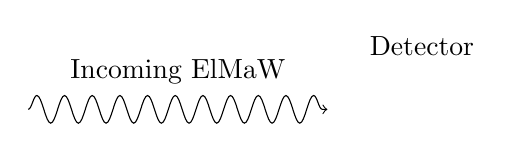
\begin{tikzpicture}
\draw[->,decorate, decoration={snake,amplitude=5,segment length=10}](0,0)--(3.8,0) node[midway,above,shift=({0,.2cm})]{Incoming ElMaW};
\detector{1}{4}{0}{0}
\node[] at (5,0.8) {Detector};
\end{tikzpicture}
\caption[][2cm]{ }
\label{fig:detectorschematic}
\end{figure}

We connect a fast oscilloscope to the detector and measure the output of the amplified electron signal. This gives us timing as to when the ElMaW kicked an electron off of the metal at the front of the detector. We might expect a signal something like Figure \ref{fig:detectorsignal} where each blip corresponds to an electron ionization event. However, when we turn up the intensity of the incoming ElMaW, we find that the signals start to overlap and eventually build up to a single, steady signal.
\begin{figure}
\centering
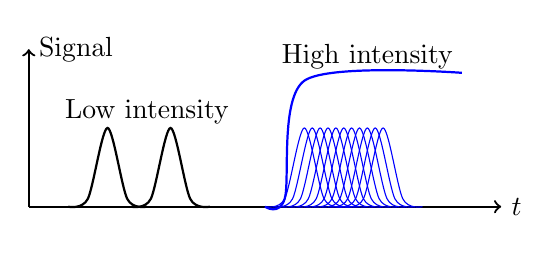
\begin{tikzpicture}
\draw[->,thick] (0,0) -- (6,0) node[right]{$t$};
\draw[->,thick] (0,0) -- (0,2) node[right]{Signal};
\draw[thick] plot[smooth] coordinates{(0.5,0)(.75,.1)(1,1)(1.25,.1)(1.5,0)};
\draw[thick,shift=({.8,0})] plot[smooth] coordinates{(0.5,0)(.75,.1)(1,1)(1.25,.1)(1.5,0)};
\draw (1.5,1.2) node{Low intensity};
\draw[thick,blue] plot[smooth] coordinates{(3,0)(3.25,.1)(3.5,1.6)(5.5,1.7)};

\foreach \a in {2.5,2.6,2.7,...,3.5}
    \draw[thin,blue,shift=({\a,0})] plot[smooth] coordinates{(0.5,0)(.75,.1)(1,1)(1.25,.1)(1.5,0)};

\draw (4.3,1.9) node{High intensity};

\end{tikzpicture}
\caption[][2cm]{ }
\label{fig:detectorsignal}
\end{figure}

\begin{example}
\label{ex:twogauss}
Model the amplified electron signal from the detector as a Gaussian pulse on the oscilloscope. What would the signal look like if two electrons arrived within the Gaussian width?
\model We will model the detector as an amplified electron coming from a metal where the electron was ejected from the surface by an ElMaW. We assume that every pulse is identical and only differs by its peak time. We model the peaks as the function: $\exp[-(t-t_k)^2/(2\sigma^2)]$ where $t_k$ is the arrival time of the $k$th pulse and $\sigma$ is the width of the pulse.

\vis The pulses will look like Figure \ref{fig:twogaussfig}.
\begin{figure}
\centering
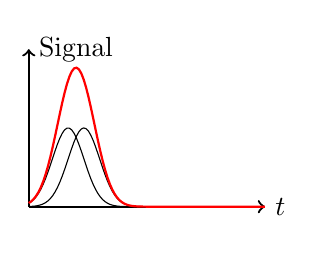
\begin{tikzpicture}
\draw[->,thick] (0,0) -- (3,0) node[right]{$t$};
\draw[->,thick] (0,0) -- (0,2) node[right]{Signal};

\draw[domain=0:3,samples=100] plot({\x},{exp(-(\x-.5)^2/(2*0.2^2))});
\draw[domain=0:3,samples=100] plot({\x},{exp(-(\x-.7)^2/(2*0.2^2))});

\draw[domain=0:3,samples=100,red,thick] plot({\x},{exp(-(\x-.7)^2/(2*0.2^2))+exp(-(\x-.5)^2/(2*0.2^2))});

\end{tikzpicture}
\caption[][2cm]{ }
\label{fig:twogaussfig}
\end{figure}

\sol We add up two Gaussians, modeling the functions as having a width of 0.2 and separated by 0.2.
\beq
\rmt{Sig}= \exp[-(t-0.5)^2/(2(0.2^2)] + \exp[-(t-0.7)^2/(2(0.2^2)]
\eeq
\assess The total signal is about twice the height and twice the width of a single pulse. That makes sense.
\end{example}

There is one more piece to this ideal detector model: we are going to ignore ``dark counts''. There are times when the detector will eject an electron even when there is no incoming ElMaW due to the thermal energy present in all objects not at absolute zero temperature. We can make this a very small effect, though, by cooling the detector. All together, we will call this the {\em ideal detector model}.\marginnote[-2cm]{A simple model for the emission of electrons is to model a ``thermionic current'' which is proportional to $T^2\E{-\Phi/kT}$ where $T$ is the detector temperature and $k$ is Boltzmann's constant.}


\begin{exercise}
What if we used a thermal detector? What would the change in temperature be if we directed an ElMaW with an intensity of 1000~W/m$^2$ on one face of an aluminum cube that is 10~cm on a side for one hour?
\end{exercise}


\chapter{Quantized Electromagnetic Waves}
Now we have most of the tools we need to explore the need for a quantum model. The one piece we are missing is a model of a beamsplitter. 
\section{Beamsplitters}
\label{sec:EMbeamsplitter}
The idea of a beamsplitter is to partially reflect and partially transmit an ElMaW. This can be accomplished with a partially silvered mirror, but they are usually made with thin film coatings so that they are less lossy.
\begin{marginfigure}\centering
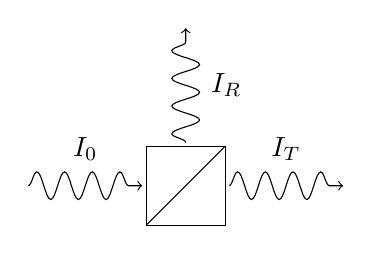
\begin{tikzpicture}
\draw (-0.5,-.5) rectangle +(1,1);
\draw (-.5,-.5) -- (.5,.5);
\draw[->,decorate, decoration={snake,amplitude=5,segment length=10, post length=.1cm}](-2,0)--(-.55,0) node[midway, above,shift=({0,.2cm})]{$I_0$};
\draw[->,decorate, decoration={snake,amplitude=5,segment length=10, post length=.1cm}](.55,0)--(2,0) node[midway, above,shift=({0,.2cm})]{$I_T$};
\draw[->,decorate, decoration={snake,amplitude=5,segment length=10, post length=.1cm}](0,.55)--(0,2) node[midway, right,shift=({.2cm,0})]{$I_R$};
\end{tikzpicture}
\end{marginfigure}
We will model our beamsplitter as having no losses and with a coating such that $I_R = I_T = I_0/2$, also known as a 50-50 beamsplitter. One of the aspects of energy conservation is that $I_R + I_T = I_0$, so we are good there.
How do we model the beamsplitter using the Complex Electromagnetic Wave Amplitude Model? We know that (Eq.~ (\ref{eq:CEWAMInt})) $I_0 = c\epsilon_0/2\abs{E_0}^2$. But this same relationship holds for $I_R = c\epsilon_0/2\abs{E_R}^2$. Relating these two, we find that
\bas
E_R = &\frac{E_0}{\sqrt{2}} \E{\I\phi_R}\;\;\rmt{and}\\
E_T = &\frac{E_0}{\sqrt{2}} \E{\I\phi_T},
\eas
where we have two arbitrary complex phases $\phi_R$ and $\phi_T$. But we also know that ElMaWs pick up a phase shift of $\pi$ on reflection, so $\phi_R - \phi_T = \pi$. To simplify our calculations, we can set $\phi_T=0$, so $\phi_R = \pi$.

\begin{example}
What are the electric field amplitudes for a 60-40 beamsplitter?

\model We model the beamsplitter as having no losses with a $\pi$ phase shift on the reflected beam. We let the 60\% arm be the reflected arm.

\vis The beamsplitter is shown in Figure \ref{fig:bsexampleprob}.

\begin{figure}
\centering
\begin{tikzpicture}
\draw (-0.5,-.5) rectangle +(1,1);
\draw (-.5,-.5) -- (.5,.5);
\draw[->,decorate, decoration={snake,amplitude=5,segment length=10, post length=.1cm}](-2,0)--(-.55,0) node[midway, above,shift=({0,.2cm})]{$I_0$};
\draw[->,decorate, decoration={snake,amplitude=5,segment length=10, post length=.1cm}](.55,0)--(2,0) node[midway, above,shift=({0,.2cm})]{$I_T = 0.4I_0$};
\draw[->,decorate, decoration={snake,amplitude=5,segment length=10, post length=.1cm}](0,.55)--(0,2) node[midway, right,shift=({.2cm,0})]{$I_R=0.6I_0$};
\caption[][2cm]{ }
\label{fig:bsexampleprob}
\end{tikzpicture}
\end{figure}

\sol So we have $I_R = 0.6 I_0$. Therefore $E_R = \sqrt{0.6}E_0 \E{\I\pi}$ and $E_T = \sqrt{0.4}E_0$.
\arnote{Make sure you work through these! I want to see your work.}

\assess When we square the amplitudes and add them, we end up back at $I_0$, so we've conserved energy. That's a good thing!

\end{example}
\begin{exercise}
What are the electric field amplitudes for beamsplitter with transmission $\alpha$ and reflection $(1-\alpha)$?
\end{exercise}

\subsection{Second-order Correlation}
\label{sec:correlation}
We split up a measurement of the output of our beamsplitter into time intervals $\Delta T$ and measure for a total time $T$. We now look at the relationship between the measured intensities of the two beams coming out of the beamsplitter and how they change (if at all) over time. This relationship, called the second-order correlation $g^{(2)}$, tells us how the two beams are related (or correlated). We are interested in the correlation between the two intensities at the same moment in time which is calculated by averaging over the time interval from $0$ to $\Delta T$ (denoted by $\avg{\;}$):
\beq
g^{(2)} = \frac{\avg{I_R(t) I_T(t)}}{\avg{I_R(t)}\avg{I_T(t)}}.
\label{eq:gtwo}
\eeq
We will use this second-order correlation to describe what is happening in our experiment setup below.

\begin{example}
What is $g^{(2)}$ if we measure a constant, equal intensity on the output of a 50-50 beamsplitter?

\model We model the beamsplitter as ideal and model the intensity as constant so that $I_R= I_T=I_0/2$. We want the second-order correlation.

\vis Constant intensities give us an intensity-versus-time graph that looks like Figure \ref{fig:constintensity}.
\begin{figure}
\centering
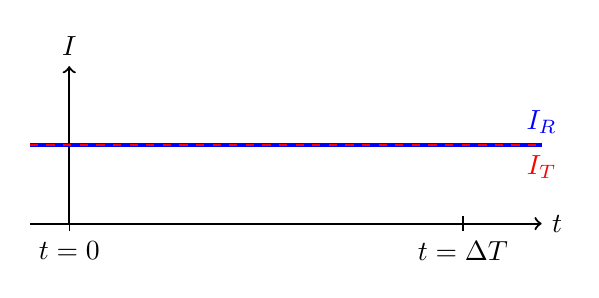
\begin{tikzpicture}[scale=1]
\draw[->,thick] (-.5,0) -- (6,0) node[right]{$t$};
\draw[->,thick] (0,0) -- (0,2) node[above]{$I$};
\draw(0,-.1) node[below] {$t=0$} -- (0,.1);
\draw(5,-.1) node[below] {$t=\Delta T$} -- (5,.1);
\draw[blue,ultra thick] (-.5,1) -- (6,1) node[above]{$I_R$};
\draw[dashed, red, thick] (-.5,1) -- (6,1) node[below]{$I_T$};

\end{tikzpicture}
\caption[][2cm]{ }
\label{fig:constintensity}
\end{figure}

\sol The average intensity over the interval is
\beq
\avg{I_R(t)} = \frac{1}{\Delta T} \int_0^{\Delta T} I_R(t) dt.
\eeq
and the same for the other average. Since both of these are constant, they are both just $I_R = I_0/2$ and $I_T=I_0/2$. Same thing with the average of the product:
\beq
\avg{I_R(t)I_T(t)} = \frac{1}{\Delta T} \int_0^{\Delta T} I_R(t)I_T(t) dt.
\eeq
So, the second-order correlation is just $g^{(2)} = 1$.\arnote{Be sure you work this through on your own from Eq.~(\ref{eq:gtwo}).}

\assess Ok, this gives us a baseline idea of what to expect for $g^{(2)}$.

\end{example}

\begin{exercise}
What is the second-order correlation for a short, gaussian-shaped pulse (like the one from Example~\ref{ex:twogauss} where the width is $0.2$ nanoseconds and the peak happens at $2.5$~ns) that is split by a 50-50 beamsplitter over a time interval of $t=0$~ns to $t=5$~ns?
\end{exercise}

We can do the same thing if we break up our time measurement into bins and measure the intensity in each bin. Then the averaging becomes a simple sum (divided by the number of bins).

\begin{exercise}
What is the second-order correlation at for the block of discrete bins shown in Table \ref{tab:normaltab}, where each bin is $100$~ns long and the intensities are all measured terms of the number of (distinct) electrons measured during the bin?
\begin{table}
\centering
\begin{tabular}{|c||c|c|c|c|c|c|c|c|c|c|c|c|}
\hline
$I_R$ & 4 & 5 & 4 & 6 & 8 & 5 & 9 & 4 & 6 & 9 & 7 & 5 \\ 
\hline
$I_T$ & 4 & 5 & 4 & 6 & 8 & 5 & 9 & 4 & 6 & 9 & 7 & 5\\
\hline
\end{tabular}
\caption[][1cm]{ }
\label{tab:normaltab}
\end{table}

\end{exercise}

\section{Coincidence Measurements}
\label{sec:coincid}
Ok. We are now ready to get at the heart of the quantum mechanic's guide. We are going to set up an experiment where we put a single trapped atom in a place where we can collect the electromagnetic waves that it emits. We will take those waves and direct them to a 50-50 beamsplitter and then put two identical detectors at the outputs of the beamsplitter.

\begin{figure}
\centering
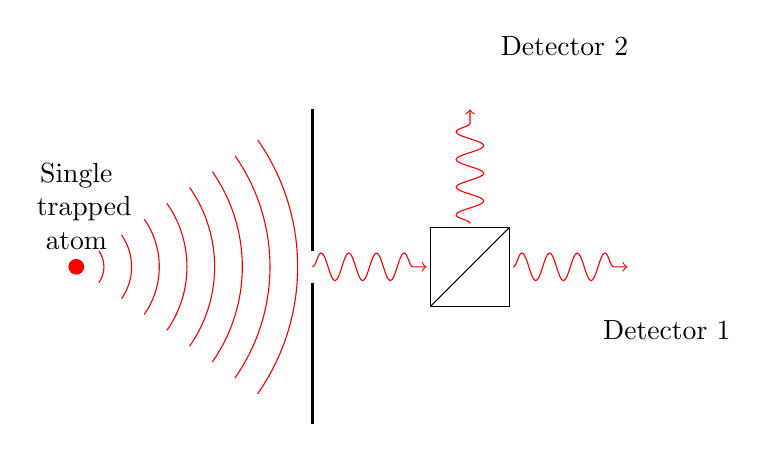
\begin{tikzpicture}
\draw (-0.5,-.5) rectangle +(1,1);
\draw (-.5,-.5) -- (.5,.5);
\draw[red,->,decorate, decoration={snake,amplitude=5,segment length=10, post length=.1cm}](-2,0)--(-.55,0) node[midway, above,shift=({0,.2cm})]{};
\draw[red,->,decorate, decoration={snake,amplitude=5,segment length=10, post length=.1cm}](.55,0)--(2,0);
\detector{1}{2.1}{0}{0}
\node at (2.5,-.8) {Detector 1};
\draw[red,->,decorate, decoration={snake,amplitude=5,segment length=10, post length=.1cm}](0,.55)--(0,2);
\detector{1}{0}{2.1}{90}
\node at (1.2,2.8) {Detector 2};
\fill[red] (-5,0) circle(0.1) node[above,black,text width=1cm,align=center,shift={(0,.1cm)}]{Single trapped atom};
\draw[red,decorate,decoration={expanding waves,angle=35}](-5,0) -- (-2,0);
\draw[thick] (-2,.2) -- (-2,2);
\draw[thick] (-2,-.2) -- (-2,-2);
\end{tikzpicture}
\end{figure}

What we measure is that we get an event on Detector 1 or Detector 2, but never on both of them at the same time. \marginnote{For experimental data on this, see, for example, PRL {\bf 39}, 691 (1977).} We measure the arrival of counts on the two detectors and count them up over a time interval. We find that each detector recorded about the same number of events and that the distribution between the two detectors is random.\marginnote{Why random? There could be ``hidden variables'' that we can't measure directly that tell which detector to record the event. There are experimental reasons that indicate that there aren't. Is the universe just weird? Are there many universes? We are going to take the ``shut up an calculate'' approach here and not worry about why questions.}

This situation calls for a new model. Nothing we've talked about prior to this point, from a classical perspective, tells us that we should expect the ElMaW to behave this way. Our classical model predicts that the wave will split at the beamsplitter and that half the intensity will go to Detector 1 and half to Detector 2.

There are lots of questions to ask: what happens to the ElMaW after the beamsplitter? Is the wave in both arms at the same time? If so, why do we not detect something at both detectors? If it is only in one arm, how do we know which? Why did it go one way and not the other? We obviously need more data.

\section{Polarizing Beamsplitter}
We use the polarization aspect of ElMaWs to say more about this new situation. We will put a polarizer between the atom and the beamsplitter so that only horizontally polarized waves pass through. Then we replace the beamsplitter with a {\em polarizing beamsplitter} (PBS). 
\begin{marginfigure}\centering
\begin{tikzpicture}[scale=1]
\draw[->,thick] (-.5,0,0) -- (4,0,0) node[right]{$x$};
\draw[->,thick] (0,0,0) -- (0,1.2,0) node[above]{$y$};
\draw[->,thick] (0,0,0) -- (0,0,1.2) node[left,below]{$z$};
\draw[color=blue,<->,thick](0,-.7,.6) -- (0,.6,-.7) node[above,black]{$\theta$};
\begin{scope}[canvas is zy plane at x=0]
\draw[dashed] (0,0,0) circle (.92);
\end{scope}
\draw[->,ultra thick](0,0,0) -- (1,0,0);
\begin{scope}[canvas is xz plane at y=.5,shift={(2,0,0)}]
\fill[black!40] (-.5,-.5) rectangle +(1,1);
\end{scope}
\begin{scope}[canvas is yz plane at x=2.5]
\fill[black!20] (-.5,-.5) rectangle +(1,1);
\end{scope}
\begin{scope}[canvas is xy plane at z=.5,shift={(2,0,0)}]
\fill[black!30] (-.5,-.5) rectangle +(1,1);
\end{scope}
\draw (1.5,.5,-.5) -- (2.5,.5,.5);
\draw (2,0,0.5) -- (2,0,2.5);
\draw[color=blue,<->,thick](3,-.5,0) -- (3,.5,0);
\draw[->,ultra thick] (2,0,.5) -- (2,0,2);
\draw[->,ultra thick] (2.5,0,0) -- (3.5,0,0);
\draw[color=blue,<->,thick](1.5,0,1.5) -- (2.5,0,1.5);
\node at (2,1.3,0) {PBS};
\end{tikzpicture}
\end{marginfigure}
This new tool reflects all of the incoming wave that has a horizontal polarization component and transmits the vertically polarized component. As with a polarizer, the transmitted electric field amplitude is $E_V = E_0 \cos\theta$ and the reflected field amplitude is $E_H = E_0 \sin\theta$. 

In terms of our setup, we arrange the PBS so that Detector 2 now gets all the horizontally polarized light and Detector 1 gets all the vertically polarized light. So, we send in horizontally polarized light and now we only measure events on Detector 2, never on Detector 1. If we rotate the initial polzarizer to be vertical, we only measure events on Detector 1, never on Detector 2. So far, so good. This is behaving like we expect for an ElMaW.

What happens down if we set the polarization angle to $\theta=\pm45^\circ$. We define these new directions as $D_R$ and $D_L$ for right- and left-diagonal.\begin{marginfigure}\centering
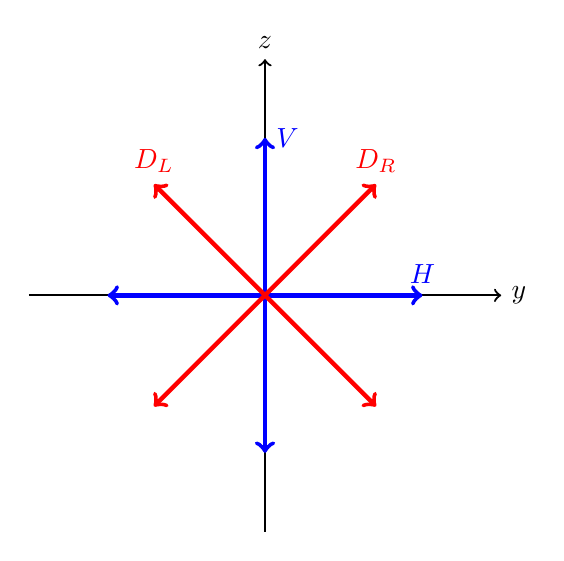
\begin{tikzpicture}[scale=1]
\draw[->,thick] (-3,0) -- (3,0) node[right]{$y$};
\draw[->,thick] (0,-3) -- (0,3) node[above]{$z$};
\draw[<->, blue,ultra thick] (-2,0) -- (2,0) node[above]{$H$};
\draw[<->, blue, ultra thick] (0,-2) -- (0,2) node[right]{$V$};
\draw[<->, red, ultra thick] (-1.41,-1.41) -- (1.41,1.41) node[above]{$D_R$};
\draw[<->, red, ultra thick] (1.41,-1.41)-- (-1.41,1.41) node[above]{$D_L$};
\end{tikzpicture}
\end{marginfigure}
With the incoming polarization set to either $D_L$ or $D_R$, we are back to measuring half of the events on Detector 1 and half on Detector 2 and never measuring an event at the same time.

\begin{exercise}
What is the second-order correlation for the following block of discrete bins measured at the output of the beamsplitter  where the intensity is measured in units of (distinct) electrons measured during the bin and where each bin is $100$~ns long?
\begin{table}
\centering
\begin{tabular}{|c||c|c|c|c|c|c|c|c|c|c|c|c|}
\hline
Detector 1 & 1 & 1 & 0 & 1 & 0 & 1 & 0 & 0 & 0 & 1 & 1 & 0 \\ 
\hline
Detector 2 & 0 & 0 & 1 & 0 & 1 & 0 & 1 & 1 & 1 & 0 & 0 & 1\\
\hline
\end{tabular}
\end{table}


\end{exercise}

\chapter{Rotated Measurements and Vector Spaces}
\section{Polarization Rotators}

We introduce a new tool here: a polarization rotator, also known as a half-wave (or $\lambda/2$) plate. What this tool does is rotate the polarization of the ElMaW without otherwise changing it. Unlike a polarizer, which blocks all the polarizations except one, a \hwp passes all polarizations, just rotating them by a specific angle $\phi$.
\begin{marginfigure}\centering
\begin{tikzpicture}[scale=1]
\draw[->,thick] (0,0,0) -- (3,0,0) node[right]{$x$};
\draw[->,thick] (0,0,0) -- (0,1,0) node[right]{$y$};
\draw[->,thick] (0,0,0) -- (0,0,1) node[right]{$z$};
\draw[color=blue,<->](.5,-.7,0) -- (.5,.7,0) node[above,black]{$\vec{E}$};
\begin{scope}[canvas is zy plane at x=1.3]
\fill[green, opacity=.2] (-1,-1) rectangle +(2,2);
\draw[dashed] (0,0) -- (0,1) node[above]{$\phi$};
\end{scope}
\draw[->,thick](1.3,0,0) node[below,text width=1cm,align=center]{\hwp}-- (1.3,.6,-.7) ;
\draw[color=blue,<->](2.3,-.45,.53) -- (2.3,.45,-.53) node[above,black]{$\vec{E}_\rmt{rotated}$};
\end{tikzpicture}
\end{marginfigure}

We take this new tool and place is before the PBS in our setup, which now looks like this:

\begin{figure}
\centering
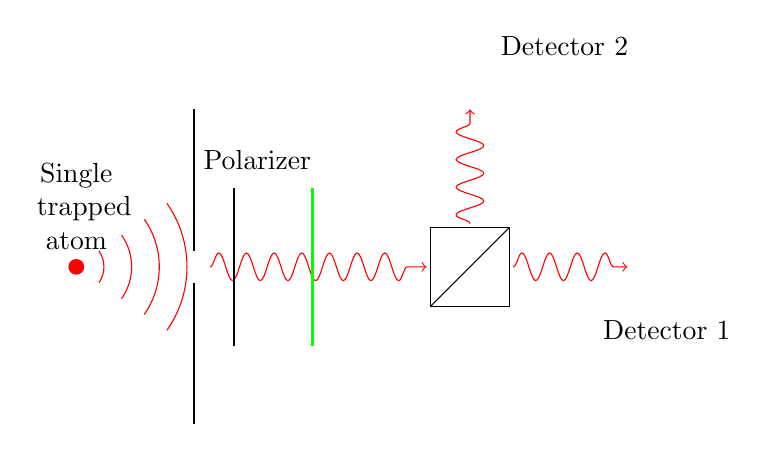
\begin{tikzpicture}
\draw (-0.5,-.5) rectangle +(1,1);
\draw (-.5,-.5) -- (.5,.5);
\draw[red,->,decorate, decoration={snake,amplitude=5,segment length=10, post length=.1cm}](-3.3,0)--(-.55,0) node[midway, above,shift=({0,.2cm})]{};
\draw[red,->,decorate, decoration={snake,amplitude=5,segment length=10, post length=.1cm}](.55,0)--(2,0);
\detector{1}{2.1}{0}{0}
\node at (2.5,-.8) {Detector 1};
\draw[red,->,decorate, decoration={snake,amplitude=5,segment length=10, post length=.1cm}](0,.55)--(0,2);
\detector{1}{0}{2.1}{90}
\node at (1.2,2.8) {Detector 2};
\fill[red] (-5,0) circle(0.1) node[above,black,text width=1cm,align=center,shift={(0,.1cm)}]{Single trapped atom};
\draw[red,decorate,decoration={expanding waves,angle=35}](-5,0) -- (-3.5,0);
\draw[thick] (-3.5,.2) -- (-3.5,2);
\draw[thick] (-3.5,-.2) -- (-3.5,-2);
\draw[thick] (-3,-1) -- (-3,1) node[above,shift={(.3,.1)}] {Polarizer};
\draw[thick,green] (-2,-1) node[below,black] {\hwp} -- (-2,1);
\end{tikzpicture}
\end{figure}

We are also going to assign a value to the measurements at each type of polarization. We will assign any measurement coming from Detector 1 as a $+1$ and any measurement from Detector 2 as a $-1$. We will use the following table to assign polarizations.
\begin{table}
\centering
\begin{tabular}{|c||c|c|}
\hline
\hwp angle & Detector 1 & Detector 2\\ 
\hline
$0^\circ$  & $V$ & $H$\\
\hline
$-45^\circ$  & $D_R$ & $D_L$\\
\hline
$90^\circ$  & $H$ & $V$\\
\hline
$45^\circ$  & $D_L$ & $D_R$\\
\hline
\end{tabular}
\end{table}

So we can now analyze the possible combinations between the polarizer angle $\theta = 0^\circ$ and the \hwp angle $\phi$ and what we get from the measurements.
\begin{itemize}
\item[\boldmath$\phi=0^\circ:$] We measure $+1$ on every measurement, 100\% of the time.
\item[\boldmath$\phi=90^\circ:$] We measure $-1$ on every measurement, 100\% of the time.
\item[\boldmath$\phi=45^\circ:$] We get a random result which is $+1$ about 50\% the time and $-1$ the other 50\%. 
\item[\boldmath$\phi=-45^\circ:$] We get a random result which is $+1$ about 50\% the time and $-1$ the other 50\%. 
\end{itemize}
We average all the measurements we get for a particular configuration. When we have probabilistic results the probability is calculated as the sum of the result value times the probability of measuring that value:

\bas
\rmt{Average Result} = & (\rmt{Result}_1)\times(\rmt{Probability of Result}_1) + \ldots \\
=& \sum_{n=1}^\rmt{All Results}(\rmt{Result}_n)(\rmt{Probability of Result}_n)
\eas

So for our $\phi=0^\circ$ case, the average is: $({+1})(1)=1$. For our $\phi=45^\circ$ case, the average is $({+1})(.5) + ({-1})(.5) = 0$. We keep adjusting the angles and find that the average results is $\cos(2\phi)$.

We interchange the detectors and find the same result. We move the detectors back and find the same result again. We obviously need a new model to describe what is going on after the the beamsplitter. We are going to call this new model a {\em Quantum State} model.\

\begin{exercise}
\label{exercise:rotatedhwp}
\begin{enumerate}
\item What are the polarizations that are measured by the  Detectors if we set the initial polarizer to $\theta=45^\circ$? Make a table like the one above for $\phi = 0^\circ, \pm 45^\circ$, and $90^\circ$. List what you expect to measure and with what probability.

\item Calculate the average results for all four $\phi$ angles from the previous part.
\end{enumerate}
\end{exercise}

\subsection{Propositions}
There is a handy piece of reasoning that we will make use of later that I want to introduce now. We start with something we can measure, like the outcome of tossing a six-sided die. This ideal die will roll $\{1,2,3,4,5,6\}$ with equal probability. We now ask questions called propositions:
\begin{itemize}
\item[Prop. A:] Is the result less than 3? It could be if it is $\{1,2\}$.
\item[Prop. B:] Is the result even? It could be if it is $\{2,4,6\}$.
\end{itemize}
We now ask {\em joint} propositions using the rules of logic.
\begin{itemize}
\item[Prop. A or B:] Is the result less than 3 {\bf or} even?  It could be if it is $\{1,2,4,6\}$.
\item[Prop. A and B:] Is the result less than 3 {\bf and} even? This is only possible if the result is $\{2\}$.
\end{itemize}

\begin{example}
Consider two propositions based on the roll of an 8-sided die:
\begin{itemize}
\item[Prop. A:] Is the result greater than 6?
\item[Prop. B:] Is the result divisible by 3?
\end{itemize}
For which measurement results will these propositions true? How about A and B as well as A or B?

\model We model the die as ideal - no result is weighted any more than any other.

\vis Not much to visualize for this problem.

\sol We have two possible results that satisfy Prop. A: ${7,8}$. There are two possible results that satisfy Prop. B: ${3,6}$. We therefore have the following joint proposition results: A {\em or} B: ${3,6,7,8}$. A {\em and} B: ${}$ - no result.

\assess The joint propositions are symmetric -- it does not matter which order we take first, A or B.

\end{example}

\section{Quantum Propositions}
\label{sec:quantprop}
We apply this same logic to the following two propositions about our measurement system where we've set the polarizer to $\theta = 0^\circ$:
\begin{itemize}
\item[Prop. A:] At $\phi=0^\circ$ do we measure ${+1}$ (or is the quantum state $V$)? Because we have the polarizer in place set to $V$ polarization, the answer to this question is that we always measure $+1$, 100\% of the time.
\item[Prop. B:] At $\phi=-45^\circ$ do we measure ${+1}$ (or is the quantum state $D_R$)? This is a little more challenging, because the answer is that sometimes we measure ${+1}$, but sometimes we measure ${-1}$, each with a 50\% probability. In any particular measurement, we might get ${+1}$, but there is no definite answer to this.
\end{itemize}
What about Prop. A or B? This is asking if the quantum state is $V$ or $D_R$. Since we will always measure a ${+1}$ for Prop. A, this joint proposition is always true. Now we try to measure Prop. A and B. We know that A is always true, since we've set the polarizer to $V$ ($\theta=0^\circ$). So we only need to adjust the \hwp to $-45^\circ$ and measure Prop. B. We find that this is ${+1}$ half the time and ${-1}$ the other half. So Prop. A and B is true 50\% of the time.

How about measuring Prop. B or A, where we reverse the order of measurement? To do this, we need to modify our  our experiment setup. Since Prop. B asks about a ${+1}$ measurement where $\phi_1=-45^\circ$, we'll leave Detector 1 where it is. In place of Detector 2, we'll add a second \hwp to rotate the polarization back to the original angle and a new set of detectors that behave just like our initial set. Detector 3 now corresponds to a ${+1}$ measurement and Detector 4 corresponds to a ${-1}$ measurement.

\begin{marginfigure}\centering
\centering
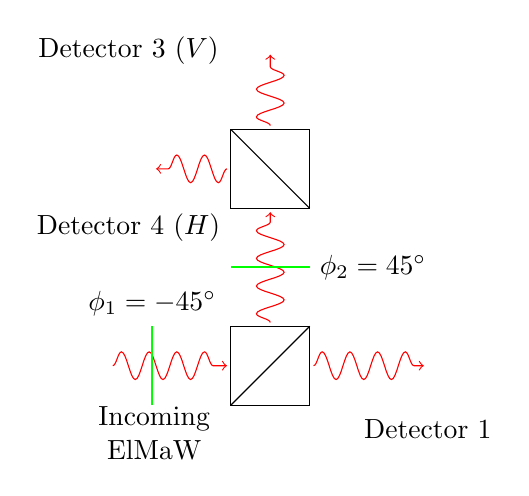
\begin{tikzpicture}
%PBS
\draw (-0.5,-.5) rectangle +(1,1);
\draw (-.5,-.5) -- (.5,.5);
%incoming beam
\draw[red,->,decorate, decoration={snake,amplitude=5,segment length=10, post length=.1cm}](-2,0)--(-.55,0) node[midway, below,shift=({-.2cm,-.4cm}),text width=2cm,black,align=center]{Incoming ElMaW};

\draw[thick,green] (-1.5,.5) node[above,black] {$\phi_1=-45^\circ$} -- (-1.5,-.5);

%outgoing beam to 1
\draw[red,->,decorate, decoration={snake,amplitude=5,segment length=10, post length=.1cm}](.55,0)--(1.95,0);
\detector{0.8}{2.1}{0}{0}
\node at (2,-.8) {Detector 1};
%beam to 2
\draw[red,->,decorate, decoration={snake,amplitude=5,segment length=10, post length=.1cm}](0,.55)--(0,1.95);

%PBS 2
\draw (-0.5,2) rectangle +(1,1);
\draw (-.5,3) -- (.5,2);

\draw[red,->,decorate, decoration={snake,amplitude=5,segment length=10, post length=.1cm}](0,3.05)--(0,3.95);

\detector{0.8}{0}{5.0}{90}
\node at (-1.8,4.0) {Detector 3 ($V$)};

\draw[red,->,decorate, decoration={snake,amplitude=5,segment length=10, post length=.1cm}](-.55,2.5)--(-1.45,2.5);
\detector{0.8}{-1.95}{3.2}{180}
\node at (-1.8,1.75) {Detector 4 ($H$)};

\draw[thick,green] (-.5,1.25) -- (.5,1.25)node[right,black] {$\phi_2=45^\circ$};

\end{tikzpicture}
\end{marginfigure}

So measuring Prop. B or A will give us ${+1}$ for B half of the time and then, since we've rotated back, will give us ${+1}$ on A half of the remaining times we measure. That means that Prop. B or A is true 75\% of the time. Compare this to the reverse which was true 100\% of the time. Clearly the ordering of our measurements matter. Our new quantum state model must take this into account and handle it. Finally, we ask about B and A. This is true 25\% of the time.\arnote{Work out this situation in your notes.}

\begin{exercise}
Consider two propositions where we have set the initial polarizer to $\theta=45^\circ$:
\begin{itemize}
\item[Prop. A:] At $\phi=0^\circ$ do we measure ${-1}$?
\item[Prop. B:] At $\phi=45^\circ$ do we measure ${+1}$?
\end{itemize}
For which measurement results will these propositions true? How about A and B as well as A or B? Finally, consider B and A as well as B or A.
\end{exercise}

\section{Linear Vector Spaces}
We are going to need a new set of mathematical tools to describe our quantum states. These are {\em vector spaces} which describe a set of relationships and interactions between the quantum states. \marginnote{A note about the word {\em vector}. We use vectors to describe position, momentum, forces, etc. in 3-space and 4-space. While that is one type of vector space, the tools we will be building here are much more general. Any time I want to refer to one of these types of vectors, I'll call it a 3-vector.} There are a number of different ways to represent a vector space in concrete form and we will make use of them as we go.

The quantum states are going to belong to a specific space of states called a {\em Hilbert Space}. We'll define this later, but it encompasses all of the possible quantum states of our system.

Our quantum vector space will be composed of elements, or states, called {\em ket-vectors} or just kets, written as $\ket{A}$. We will make use of complex numbers in this vector space and will represent them as $z$ and $w$.

In the quantum vector space, the following relationships hold between quantum states:\marginnote{We are following Susskind here.}
\begin{enumerate}
\item The sum of two kets is another ket:
\beq
\ket{A} + \ket{B} = \ket{C}
\eeq
\item Addition is commutative:
\beq
\ket{A} + \ket{B} = \ket{B} + \ket{A}
\eeq
\item Addition is associative:\marginnote{All of these relationships hold for 3-vectors, but where we only allow multiplication by real numbers.}
\beq
\left(\ket{A} + \ket{B}\right) +\ket{C} = \ket{A} + \left(\ket{B} + \ket{C}  \right)
\eeq
\item There exists a $0$ ket (usually written without the $\ket{\,}$) such that addition by it doesn't change a ket-vector:
\beq
\ket{A} + 0 = \ket{A}
\eeq
\item There exists a ``negative'' ket such that when you add to the positive ket, you get zero:
\beq
\ket{A} + \left({-\ket{A}} \right) = 0
\eeq
\item Multiplication by a complex number gives a new ket (note there are two equivalent ways of writing the multiplication):
\beq
z\ket{A} \equiv \ket{zA} = \ket{B}
\eeq
\item Multiplication by a complex number is distributive in a linear fashion:\marginnote{These last two constitute the conditions known as linearity.}
\beq
z\left(\ket{A} + \ket{B}  \right) = z\ket{A} + z\ket{B}
\eeq
\item and the same way here, too:
\beq
(z+ w)\ket{A} = z\ket{A} + w\ket{A}.
\eeq
\end{enumerate}

Wow, that was really abstract. There are a couple of ways we can make this more concrete. One way is to use complexe valued functions of some variable $x$. We'll explore these first:

\begin{example}
Show that $A(x) = 3+ \I x$ and $B(x) = 4 x - 6\I$ are both vector spaces.

\model We will model these two functions as complex functions of a real number $x$.

\vis Rats. It is hard to visualize things now. However, both of these functions are lines in the complex plane:
\begin{figure}
\centering
\begin{tikzpicture}[scale=0.3]
\draw[->,thick] (-10,0) -- (10,0) node[right]{Real};
\draw[->,thick] (0,-10) -- (0,10) node[above]{Imaginary};
\draw[color=blue,domain=-10:10] plot (3,\x);
\node[blue] at (5,1) {$A(x)$};
\draw[color=red,domain=-2.5:2.5] plot ({4*\x},-6);
\node[red] at (-6,-5) {$B(x)$};
\draw[color=green,domain=-2.5:2.5] plot ({3+4*\x},{\x-6});
\node[green] at (9,-3) {$(A+B)$};
\end{tikzpicture}
\end{figure}

\sol We just have to work through each of the pieces that make up a vector space and make sure that we end up with another complex-valued function. Here's the first two:
\begin{enumerate}
\item $\ket{A} + \ket{B} =  (3+ \I x) + (4 x - 6\I) = [3+4x + \I(x-6)]$ which is another complex-valued function (shown in green on the figure)
\item $\ket{B} + \ket{A} =   (4 x - 6\I) + (3+ \I x)  = [3+4x + \I(x-6)]$ which is the same thing we got before.\arnote{Your turn. Finish up the rest of these as practice.}
\end{enumerate}
\assess We stayed in the vector space for all the points which means that this type of linear, complex-valued function works as a concrete representation of a vector space.
\end{example}

\begin{exercise}
Show that a quadratic complex-valued function (you can invent your own as long as they have some kind of $x^2$ in them somewhere) also works to represent a vector space.
\end{exercise}

Another way we represent the vector space in a concrete form is to use matrices. We represent the ket as a column matrix. For simplicity we will make it a 1 by 2 matrix where each element $\alpha_k$ is a complex number.\marginnote{We will use the symbol $\Meq$ when we represent a vector with a matrix. It isn't really an equals because we are changing representations, but close.}
\beq
\ket{A}\Meq\vket{\alpha_1}{\alpha_2}
\eeq
This representation of a vector space also fulfills our requirements. For example:\arnote{Finish up showing that the matrix representation of the vector space also works for all the requirements.}
\beq
\ket{A} + \ket{B} \Meq \vket{\alpha_1}{\alpha_2} + \vket{\beta_1}{\beta_2} = \vket{\alpha_1 + \beta_1}{\alpha_2+\beta_2}
\eeq
and
\beq
z\ket{A}\Meq z\vket{\alpha_1}{\alpha_2} = \vket{z\alpha_1}{z\alpha_2}.
\eeq

\subsection{Bras and Kets}

We define a new vector space, related to the ket-vector called a {\em bra-vector} or a bra for short. These are writte as: $\bra{A}$ and follow all the same rules as the kets. The bra-vectors are related to the ket-vectors in the following way. In order to flip from a ket to a bra, we take the complex conjugate and we also reverse any ordering like this:
\beq
z\ket{A}\rightarrow \bra{A}z^*.
\eeq

In terms of our concrete matrix representation, we need to take the complex conjugate of all the elements {\em and} turn the column vector into a row vector.
\bas
\ket{A} \rightarrow & \bra{A} \\
\vket{\alpha_1}{\alpha_2} \rightarrow &  \vbra{\alpha_1^*}{\alpha_2^*}
\eas

\begin{exercise}
Show that the following two complex matrix vectors satisfy the requirements for our vector space:
\beq
\begin{pmatrix} 1+3\I \\ -4-\I \\ 7+6\I \end{pmatrix} \rmt{ and } 
\begin{pmatrix} 6 \\ 8+\I \\ -5\I \end{pmatrix}.
\eeq
\end{exercise}

\chapter{Quantum States and Vectors}

We continue developing the mechanics of working with vector spaces, then we will apply these to our quantum states.

\section{Inner Products}

We also define an inner product between a bra and a ket. This gives us a {\em bra-ket} or a bracket, which is where the names bra a ket come from. The inner product, or dot product, of two 3-vectors tells us how much one of the vectors lies along the direction of the other. The inner product takes two vectors as inputs and returns a complex number as the output.
\begin{marginfigure}\centering
\begin{tikzpicture}[scale=1]
\draw[->,red] (0,0) -- (3,1) node[right,black]{$\vec{V}_1$};
\draw[->,blue] (0,0) -- (1.8,2.8) node[above,black]{$\vec{V}_2$};

\draw [dashed] ($(0,0)!(1.8,2.8)!(3,1)$) coordinate(B) -- (1.8,2.8);

\draw[->,dashed,thick] (0,0)--(B);

\end{tikzpicture}
\end{marginfigure}
We note the inner product between a bra and a ket as
\bas
\bra{A}\ket{B}\equiv \avg{A|B}.
\eas
If we reverse the order of the inner product, we have to take the complex conjugate of the output in order to follow our bra-to-ket rule above: $\avg{A|B} = \avg{B|A}^*$.

The representation of the inner product in terms of matrices is the product of a row matrix (the bra) and a column matrix (the ket):
\beq
\avg{A|B}\Meq\vbra{\alpha_1^*}{\alpha_2^*}\vket{\beta_1}{\beta_2} = \alpha_1^*\beta_1 + \alpha_2^*\beta_2
\eeq\marginnote[-1cm]{In terms of 3-vectors, the dot product of two vectors in terms of their components is $\vec{a}\cdot\vec{b}=a_x b_x + a_yb_y + a_zb_z$.}

\subsection{Normalization}
Following a couple of other definitions from 3-vectors, we can talk about the ``magnitude'' of a state vector in our quantum state space by taking the inner product of a state vector with itself: $\avg{A|A}$. We are mostly going to be working with state vectors that are {\em normalized}, where their magnitude is $1$:
\beq
\avg{A|A} = 1.
\eeq

\subsection{Orthogonality}
We also borrow the idea of two state vectors being {\em orthogonal} from our 3-vector concepts. Two 3-vectors are orthogonal if their dot product is zero. We define a similar concept for our state vectors. $\ket{A}$ and $\ket{B}$ are orthogonal if
\beq
\avg{A|B} = 0.
\eeq

\begin{exercise}
\label{ex:statevector}
You are given the quantum state 
\beq
\ket{A} \Meq \vket{2+3\I}{-4}.
\eeq
\begin{enumerate}
\item Normalize the state vector.
\item Find another normalized state vector that is orthogonal to $\ket{A}$
\end{enumerate}
\end{exercise}

\section{Orthonormal Basis Vectors}

It is really handy when we work with 3-vectors to break a vector up in terms of its components in some orthogonal basis of unit vectors. For example, we can write the vector $\vec{V}$ as $\vec{V} = V_x\hat{x} + V_y\hat{y} + V_z\hat{z}$. \marginnote{We could have picked a different basis, for example, polar basis 3-vectors: $\vec{V}=V_r\hat{r}+V_\theta\hat{\theta}+V_\phi\hat{\phi}$. The same thing applies to this set of orthonormal basis 3-vectors.} The unit vectors all have the properties where they are normalized: $\hat{x}\cdot\hat{x}=1$ and they are orthogonal: $\hat{x}\cdot\hat{y}=0$. We put both of these together and call the set of basis 3-vectors {\em orthonormal}.
We write our 3-vector in terms of these basis 3-vectors by finding the piece of the 3-vector that lies along the basis vector ($V_x = \vec{V}\cdot\hat{x}$), repeating the same thing for the other basis 3-vectors, then adding them together.

We now do the same thing for our quantum state vectors. We want to work in general, so we won't be specific yet about the representation of our basis vectors, but we'll be able to specify them later. For now, we will say we have a set of basis vectors $\ket{j}$.\marginnote[-1cm]{We can do this with 3-vectors by defining $\hat{x}_j$ where $j=1,2,3$ and $\hat{x}_1 \equiv \hat{x}$, $\hat{x}_2\equiv\hat{y}$, etc.} We decompose any quantum state vector in terms of the basis vectors in the same way as with 3-vectors:
\toolnote{\toollabel{tool:decom}{\includegraphics{tool1.tikz} {\bf Orthonormal Basis Decomposer}}  This tool is used to write a state vector in terms of a set of orthonormal basis vectors.} 
\beq
\ket{A} = \sum_j \alpha_j \ket{j},
\label{eq:decom}
\eeq
where $\alpha_j$ are complex numbers replacing the $V_x$, $V_y$, etc. from the 3-vector example.

We follow our pattern from 3-vectors to figure out what the $\alpha_j$ complex numbers should be in our $\ket{j}$ basis. We first need to do two things: 1) define the bra version of the basis which we will call $\bra{k}$. \marginnote{Note that $\bra{j}$ and $\bra{k}$ are both in the same set of possible basis states.} We now take the inner product of this basis bra-vector with our state vector:
\beq
\avg{k|A}=\sum_j\bra{k}\alpha_j \ket{j}.
\eeq
Now we can use the fact that our basis vectors are orthogonal so that if $k=j$ then $\avg{j|j}=1$. Otherwise, $\avg{k|j}=0$. We can write this in terms of the Kronecker delta:
\beq
\delta_{kj} = \begin{cases}1 &\rmt{ if } j=k, \\ 0 &\rmt{ if }j\neq k.\end{cases}
\label{eq:kronecker_eqn}
\eeq
So we now have $\avg{k|j}=\delta_{kj}$. This is a very useful tool since now the sum over $j$ simplifies. The only term that isn't zero is the one where $k=j$, and that one is just $\alpha_{k}$. This is a new tool, written in general gives us
\toolnote{\toollabel{tool:orthog}{\includegraphics{tool2.tikz} {\bf Orthonormal Collapser}}  This tool is used to collapse a sum using the inner product of two orthonormal state vectors.} 
\beq
\avg{k|A} = \bra{k} \left( \sum_j \alpha_j \ket{j} \right)= \alpha_k.
\label{eq:orthog}
\eeq
So we have (replacing $k$ with $j$ to emphasise that it doesn't matter what symbol we use to describe our basis states)
\beq
\avg{j|A} = \alpha_j.
\eeq

There is one more trick we can use here. We insert this back into our decomposition of $\ket{A}$ in terms of its basis vectors, Eq.~(\ref{eq:decom})
\beq
\ket{A} = \sum_j\avg{j|A}\ket{j}.
\eeq
Since $\avg{j|A}$ is just a complex number, we can write it before or after the vector. So we write it after and get
\beq
\ket{A} = \sum_j \ket{j}\bra{j} \ket{A}.
\eeq
This implies that the combination of the sum and the ket-bra vectors must be $1$. This is a really useful tool that we will come back to again and again.
\toolnote{\toollabel{tool:span}{\includegraphics{tool3.tikz} {\bf Completeness Spanner}}  This tool is used to insert a complete set of basis vectors and project a state vector onto that basis.} 
\beq
\sum_j \ket{j}\bra{j} = 1
\label{eq:span}
\eeq
This is also known as the completeness relationship because it works since the basis vectors $\ket{j}$ form a complete basis.

Now that we have this handful of tools, we are ready to go back to our quantum ElMaW system and use these tools to model that system.

\begin{example}
I give you a complete set of orthonormal basis vectors: $\{\ket{0},\ket{1},\ket{2},\ket{3},\ket{4} \}$ and a vector $\ket{A} = 3\ket{0} + 2\I \ket{1} + (-3+4\I)\ket{3} - 6\ket{4} $ decomposed in this basis.
\begin{enumerate}
\item Show that the orthogonality collapser, Eq.~(\ref{eq:orthog}), gives the components of the vector $\ket{A}$.
\item Show that the completeness spanner, Eq.~(\ref{eq:span}), equal $1$.
\end{enumerate}

\model We are modeling the given set of basis vectors as being complete- they cover all possibilities in our Hilbert space.

\vis It is hard to visualize a 5-dimensional vector space, though it is just a vector pointing is some direction.

\sol We first want to use the \ref{tool:orthog} tool to decompose the vector into its basis states. We begin by projecting each one of the basis vectors onto our given vector $\ket{A}$. We start with the $\bra{0}$ basis vector:
\beq
\avg{0|A} =  3\avg{0|0} + 2\I \avg{0|1} + 0 \avg{0|2} + (-3+4\I)\avg{0|3} - 6\avg{0|4} = 3, 
\eeq
because of the nature of the orthogonal basis vectors (Eq.~(\ref{eq:kronecker_eqn}). We continue with the other basis vectors to get
\bas
\avg{1|A} =& 2\I & \avg{2|A} =& 0 \\
\avg{3|A} = & (-3+4\I) & \avg{4|A} = & -6
\eas

We now try out the \ref{tool:span} tool. This means we multiply out
\beq
\left(\sum_j \ket{j}\bra{j}\right)\ket{A} = \left( \ket{0}\bra{0} +\ket{1}\bra{1} +\ket{2}\bra{2} +\ket{3}\bra{3} +\ket{4}\bra{4}   \right) \ket{A}.
\eeq
We simplify our calculations noting that the only terms that will be non-zero are the terms like $\ket{0}\bra{0}\ket{0}$ since the other terms like $\ket{3}\bra{3}\ket{1}$ are zero due to the orthogonality condition of the basis vectors. After we expand out the product and simplify we are left with\arnote{Write out this product in your notes and make sure you get this result.}
\beq
\left(\sum_j \ket{j}\bra{j}\right) \ket{A} = 3\ket{0} + 2\I \ket{1} + (-3+4\I)\ket{3} - 6\ket{4} 
\eeq

\assess This gives us $\ket{A}$, so we find that the\ref{tool:span} must be 1, as expected.

\end{example}

\section{Modeling Quantum States}

We go back to our ElMaW model where we look at the emission of an electromagnetic wave from a single atom. The wave passes through a polarizer (angle $\theta$), then a \hwp (angle $\phi$), then to our PBS and our detectors.
\begin{marginfigure}\centering
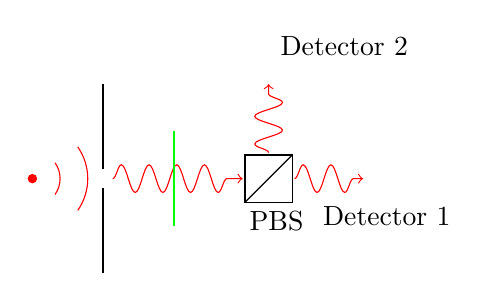
\begin{tikzpicture}[scale=0.6]
\draw (-0.5,-.5) rectangle +(1,1) node[below,shift={(-.2,-.6)}]{PBS};
\draw (-.5,-.5) -- (.5,.5);
\draw[red,->,decorate, decoration={snake,amplitude=5,segment length=10, post length=.1cm}](-3.3,0)--(-.55,0) node[midway, above,shift=({0,.2cm})]{};
\draw[red,->,decorate, decoration={snake,amplitude=5,segment length=10, post length=.1cm}](.55,0)--(2,0);
\detector{1}{2.1}{0}{0}
\node at (2.5,-.8) {Detector 1};
\draw[red,->,decorate, decoration={snake,amplitude=5,segment length=10, post length=.1cm}](0,.55)--(0,2);
\detector{1}{0}{2.1}{90}
\node at (1.6,2.8) {Detector 2};
\fill[red] (-5,0) circle(0.1);
\draw[red,decorate,decoration={expanding waves,angle=35}](-5,0) -- (-3.5,0);
\draw[thick] (-3.5,.2) -- (-3.5,2);
\draw[thick] (-3.5,-.2) -- (-3.5,-2);
%\draw[thick] (-3,-1) -- (-3,1) node[above,shift={(.5,.1)}] {Polarizer};
\draw[thick,green] (-2,-1) node[below,black] {\hwp} -- (-2,1);
\end{tikzpicture}
\end{marginfigure}
Now we remove the polarizer and set \hwp to $0^\circ$. We get results ${\pm 1}$ on the two detectors. We now define the states where we measure ${+1}$ as the state vector $\ket{V}$ and the states where we measure ${-1}$ as $\ket{H}$.

\subsection{Paramatrization}

Are $\ket{V}$ and $\ket{H}$ a complete set of basis vectors? How many basis vectors do we need to describe the direction of the polarization? For a free propagating ElMaW, there are two degrees of freedom. For a general 3-vector, there are also two degrees of freedom (the polar angles $\theta$ and $\phi$). So we need two parameters to specify an arbitrary quantum state. We will write the state as
\beq
\ket{A} = \alpha_V\ket{V} + \alpha_H\ket{H}
\label{eq:adecomp}
\eeq\marginnote[-1cm]{Using \ref{tool:decom}}%
where $\alpha_H$ and $\alpha_V$ are complex numbers. \marginnote[1cm]{This may look like 4 parameters (two complex numbers), but it is only 2 since we will need to normalize $\ket{A}$ and since there is an overall arbitrary complex phase factor since $\E{\I\beta}\E{-\I\beta}=1$.} So, $\ket{V}$ and $\ket{H}$ look like they might work for basis vectors. Are they normalized? What is $\avg{V|V}$? We know that if we start with a $V$-polarized wave and send it through a $V$ polarizer, it doesn't change the polarization. That is good evidence that $\avg{V|V}=1$. 

Are $\ket{V}$ and $\ket{H}$ orthogonal? If we send a $V$-polarized wave through a $H$ polarizer, none of the wave passes. That looks like evidence that $\avg{V|H}=0$.

\section{Probabilities}

Going back to our arbitrary state vector $\ket{A} = \alpha_H\ket{H}+\alpha_V\ket{V} $, we use the Orthogonality Collapser to see what happens when we send the $\ket{A}$ through a $V$-oriented polarizer:
\beq
\begin{split}
\avg{V|A} &= \alpha_V \rmt{ and likewise}\\
\avg{H|A} &= \alpha_H
\end{split}
\label{eq:vandhcomponents}
\eeq\marginnote[-1.5cm]{Using \ref{tool:orthog}}%
This seems to indicate that $\alpha_V$ and $\alpha_H$ are related to what we measure on our detectors. But they are complex numbers, which isn't good for a probability --- we can't measure complex probabilities. We will, instead, define the probability $P$ of measuring 
\beq
P(\rmt{measuring }{+1} \rmt{ \ie } \ket{V}) = \alpha_V^*\alpha_V.
\label{eq:ampprob}
\eeq
We use a bit of complex notation shorthand ($\alpha_V^*\alpha_V = \abs{\alpha_V}^2$) and Eq.~(\ref{eq:vandhcomponents}) to write $\alpha_V=\avg{V|A}$ which gives us a new tool for predicting the probability of measuring a particular outcome:
\toolnote{\toollabel{tool:prob}{\includegraphics{tool4.tikz} {\bf Probability Predictor}}  This tool is used to calculate the probability of measuring a particular outcome of a quantum state.}%
\beq
P(\rmt{measuring } \ket{V}) = \abs{\avg{V|A}}^2.
\label{eq:prob}
\eeq%
It is important to note that we've set the \hwp to $0^\circ$. That means we are measuring in the $V-H$ basis and it makes sense to use $\ket{H}$ and $\ket{V}$ as our orthonormal basis states.

Ok, what do we get now if we check the normalization of $\ket{A}$?\arnote[.5cm]{Expand the parenthesis and then use the orthonormal nature of $\ket{V}$ and $\ket{H}$ to simplify.}
\bas
\avg{A|A} = &\left(\bra{H}\alpha_H^* +\bra{V}\alpha_V^*\right)\left(\alpha_H\ket{H}+\alpha_V\ket{V}\right)\\ =& \alpha_H^*\alpha_H + \alpha_V^*\alpha_V 
\eas
But we make sure that all of our quantum state vectors are all normalized so that $\avg{A|A}=1$. Combining this with Eq~(\ref{eq:ampprob}) gives us
\beq
P(\rmt{measuring } \ket{V}) + P(\rmt{measuring } \ket{H}) =1.
\eeq
This is good. It means that we have a 100\% chance of measuring something.

\begin{exercise}
Starting with the quantum state 
\beq\ket{A} = \frac{1+\I}{\sqrt{3}} \ket{V} + \frac{\I}{\sqrt{3}}\ket{H},
\eeq

\begin{enumerate}
\item Check that $\ket{A}$ is normalized.
\item What is the probability of measuring $\ket{V}$?
\item What is the probability of measuring $\ket{H}$?
\item Is the total probability equal to $1$?
\end{enumerate}

\end{exercise}

\section{A Second Orthonormal Basis}
\begin{marginfigure}[2cm]
\centering
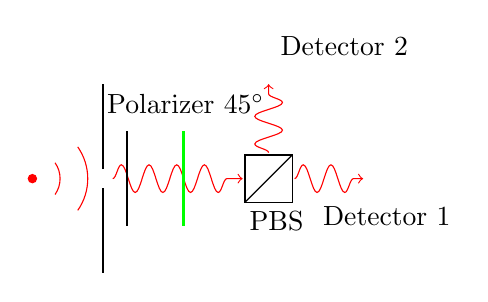
\begin{tikzpicture}[scale=0.6]
\draw (-0.5,-.5) rectangle +(1,1) node[below,shift={(-.2,-.6)}]{PBS};
\draw (-.5,-.5) -- (.5,.5);
\draw[red,->,decorate, decoration={snake,amplitude=5,segment length=10, post length=.1cm}](-3.3,0)--(-.55,0) node[midway, above,shift=({0,.2cm})]{};
\draw[red,->,decorate, decoration={snake,amplitude=5,segment length=10, post length=.1cm}](.55,0)--(2,0);
\detector{1}{2.1}{0}{0}
\node at (2.5,-.8) {Detector 1};
\draw[red,->,decorate, decoration={snake,amplitude=5,segment length=10, post length=.1cm}](0,.55)--(0,2);
\detector{1}{0}{2.1}{90}
\node at (1.6,2.8) {Detector 2};
\fill[red] (-5,0) circle(0.1);
\draw[red,decorate,decoration={expanding waves,angle=35}](-5,0) -- (-3.5,0);
\draw[thick] (-3.5,.2) -- (-3.5,2);
\draw[thick] (-3.5,-.2) -- (-3.5,-2);
\draw[thick] (-3,-1) -- (-3,1) node[above,shift={(.75,.1)},text width=2cm, align=left] {Polarizer $45^\circ$};
\draw[thick,green] (-1.8,-1) node[below,black] {\hwp} -- (-1.8,1);
\end{tikzpicture}
\end{marginfigure} We return back to our setup and this time we add the polarizer back in and turn it to $45^\circ$.\marginnote{We saw in Exercise \ref{exercise:rotatedhwp} that we needed to put the \hwp at ${-45}^\circ$ in order to measure in this basis.} This means we are preparing a new, specific state with polarization $D_R$. We know from our previous experiments that we should expect to measure ${+1}$ half of the time and to measure ${-1}$ the other half, with random results on each measurement. Using our probability model, we expect that the quantum state after the polarizer to be something like
\beq
\ket{D_R} = \frac{1}{\sqrt{2}}\ket{V} + \frac{1}{\sqrt{2}}\ket{H}.
\label{eq:drcomp}
\eeq
That state has everything we need in it - the probabilities all work out and the measurements we get from it agree with our experiment results and it is normalized. Is there another normalized basis vector $\ket{D_L}$ that is orthogonal to $\ket{D_R}$? We write $\ket{D_L}$ as an arbitrary vector $\ket{D_L} = \alpha_H\ket{H} + \alpha_V\ket{V}$ and then take the inner product with $\ket{D_R}$ and set that to zero. Doing this we find that \arnote{Do this on your own and check your work!}
\beq
\ket{D_L}  = \frac{1}{\sqrt{2}}\ket{V} - \frac{1}{\sqrt{2}}\ket{H}.
\label{eq:dlcomp}
\eeq

We are doing all of these measurements in the $V-H$ basis with the \hwp at $0^\circ$. We could, however, rotate the \hwp to $-45^\circ$ and measure in the $D_R-D_L$ basis. We can invert these two equations to see what $\ket{H}$ and $\ket{V}$ would be in this basis. We get\arnote{You need to work this one, too!}
\bas
\ket{V} =&\frac{1}{\stwo}\ket{D_R} + \frac{1}{\stwo}\ket{D_L}\\
\ket{H} =& \frac{1}{\stwo}\ket{D_R} - \frac{1}{\stwo}\ket{D_L}.
\eas
%
\begin{example} 
What is the arbitrary vector $\ket{A} = \frac{4}{5}\ket{V} + \frac{3\I}{5} \ket{H}$ in the $D_R-D_L$ basis?

\model We are given a state prepared in the $V-H$ basis, so we model this with the polarizer at some angle $\theta$ that gives us this state. We set the \hwp at ${-45}^\circ$ to measure in the $D_R-D_L$ basis.

\vis Our picture is the same as we've used before, shown in Figure \ref{fig:polexamplefig}.
\begin{figure}
\centering
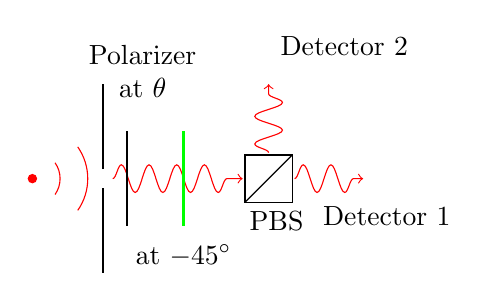
\begin{tikzpicture}[scale=0.6]
\draw (-0.5,-.5) rectangle +(1,1) node[below,shift={(-.2,-.6)}]{PBS};
\draw (-.5,-.5) -- (.5,.5);
\draw[red,->,decorate, decoration={snake,amplitude=5,segment length=10, post length=.1cm}](-3.3,0)--(-.55,0) node[midway, above,shift=({0,.2cm})]{};
\draw[red,->,decorate, decoration={snake,amplitude=5,segment length=10, post length=.1cm}](.55,0)--(2,0);
\detector{1}{2.1}{0}{0}
\node at (2.5,-.8) {Detector 1};
\draw[red,->,decorate, decoration={snake,amplitude=5,segment length=10, post length=.1cm}](0,.55)--(0,2);
\detector{1}{0}{2.1}{90}
\node at (1.6,2.8) {Detector 2};
\fill[red] (-5,0) circle(0.1);
\draw[red,decorate,decoration={expanding waves,angle=35}](-5,0) -- (-3.5,0);
\draw[thick] (-3.5,.2) -- (-3.5,2);
\draw[thick] (-3.5,-.2) -- (-3.5,-2);
\draw[thick] (-3,-1) -- (-3,1) node[above,shift={(.2,.3)},text width=2cm, align=center] {Polarizer at $\theta$};
\draw[thick,green] (-1.8,-1) node[below,black,text width=2.5cm, align=center,shift={(0,-.1)}] {\hwp at ${-45}^\circ$} -- (-1.8,1);
\end{tikzpicture}
\caption[][2cm]{ }
\label{fig:polexamplefig}
\end{figure}

\sol We use the relationships between the two basis sets to plug in for $\ket{V}$ and $\ket{H}$. Simplifying, we get \arnote{More things for you to work out! Both the substitution and the normalization.}
\beq
\ket{A} = \frac{4+3\I}{5\sqrt{2}} \ket{D_R} + \frac{4-3\I}{5\sqrt{2}} \ket{D_L}. 
\eeq

\assess We better check the normalization of our state:
\bas
\avg{A|A} =& \left(\frac{4-3\I}{5\sqrt{2}} \bra{D_R} + \frac{4+3\I}{5\sqrt{2}} \bra{D_L}\right) \left(\frac{4+3\I}{5\sqrt{2}} \ket{D_R} + \frac{4-3\I}{5\sqrt{2}} \ket{D_L}\right)\\
=& 1.
\eas
Our normalization works. Good.

\end{example}
%

%
\begin{exercise}
What are the probabilities of measuring ${+1}$ and ${-1}$ if we send the following state: 
$\ket{A} = \frac{\I}{2}\ket{V} + \frac{\sqrt{3}}{2}\ket{H}$ into our measurement system with the \hwp at ${-45}^\circ$?

\end{exercise}


\section{One more Basis}
\label{sec:ybasis}
We now have two different sets of basis vectors. But, in principle, the polarization of the ElMaW could point in one more direction! This is known as {\em circular} polarization and it corresponds to a phase shift between the $x$ and $y$ components of the electric field vector. This is written (using the CEWAM) as either {\em right-handed}
\begin{marginfigure}\centering
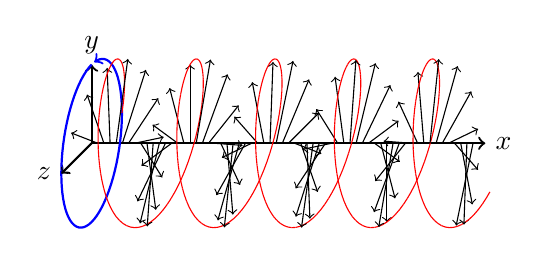
\begin{tikzpicture}[scale=1]
\draw[->,thick] (0,0,0) -- (5,0,0) node[right]{$x$};
\draw[->,thick] (0,0,0) -- (0,1,0) node[above]{$y$};
\draw[->,thick] (0,0,0) -- (0,0,1) node[left]{$z$};

\draw [->,thick,blue] (0,1,0) \foreach \t in {0,5,...,355}{
        -- (0,cos \t, sin \t) } ;

\foreach \k [evaluate={%
    \i=\k*5.625; 
    \j=\i>0 ? \i-5.625 : 0; 
    \a=90-\i; 
    \b=90-\j; 
    \c=int(mod(\k,5));}] 
    in {0,...,310}{
        \ifnum\c=0
            \draw [->] (\i/360,0,0) -- ++(0,cos \a, sin \a);
        \fi
        \draw [red] (\i/360,cos \a, -sin \a) -- (\j/360,cos \b, -sin \b);
    }
\end{tikzpicture}
\end{marginfigure}

\beq
\vec{E}_{C_R} = \frac{1}{\stwo}E_0\E{\I(kx-\omega t)}(\hat{y} + \I \hat{z})
\eeq
or as {\em left-handed} circular polarization:
\begin{marginfigure}\centering
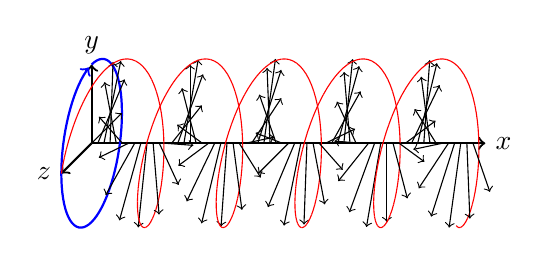
\begin{tikzpicture}[scale=1]
\draw[->,thick] (0,0,0) -- (5,0,0) node[right]{$x$};
\draw[->,thick] (0,0,0) -- (0,1,0) node[above]{$y$};
\draw[->,thick] (0,0,0) -- (0,0,1) node[left]{$z$};

\draw [->,thick,blue] (0,1,0) \foreach \t in {0,5,...,355}{
        -- (0,cos \t, -sin \t) } ;

\foreach \k [evaluate={%
    \i=\k*5.625; 
    \j=\i>0 ? \i-5.625 : 0; 
    \a=90-\i; 
    \b=90-\j; 
    \c=int(mod(\k,5));}] 
    in {0,...,310}{
        \ifnum\c=0
            \draw [->] (\i/360,0,0) -- ++(0,cos \a, -sin \a);
        \fi
        \draw [red] (\i/360,cos \a, sin \a) -- (\j/360,cos \b, sin \b);
    }
\end{tikzpicture}
\end{marginfigure}
\beq
\vec{E}_{C_L} = \frac{1}{\stwo}E_0\E{\I(kx-\omega t)}(\hat{y} - \I \hat{z})
\eeq

Experimentally, we can turn linear polarization into circular polarization using a {\em quarter wave-plate} also written as a \qwp. We place the \qwp  between the polarizer and the \hwp. If we set the \qwp to $C_R$ or $C_L$ polarization, then it doesn't matter whether we measure in the $V-H$ or the $D_R-D_L$ basis, we measure half of the events at Detector 1 and half at Detector 2. This is evidence that the $C_R-C_L$ basis is orthogonal to both of the other bases. Because the ElMaW can point in any direction in 3-vector space, we need one more orthonormal set of basis vectors to cover all the possibilities. One set that works is:
\bas
\ket{C_R} = & \frac{1}{\stwo}\ket{V} + \frac{\I}{\stwo}\ket{H} \\
\ket{C_L} = & \frac{1}{\stwo}\ket{V} - \frac{\I}{\stwo}\ket{H}.
\label{eqn:circular_pol_basis}
\eas
%
\begin{example}
Does the model for circularly polarized quantum states work? 
\begin{enumerate}
\item Is it orthonormal?
\item Is it orthogonal to the other bases?
\item Does it make the expected prediction for measurement results?
\end{enumerate}

\model We will use the basis decomposition given in Eq.~(\ref{eqn:circular_pol_basis}) and work this out using the $\ket{V}$ and $\ket{H}$ basis, which we know is orthonormal.
\begin{marginfigure}
\centering
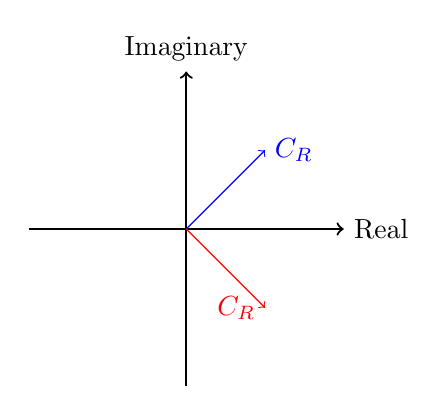
\begin{tikzpicture}[scale=0.2]
\draw[->,thick] (-10,0) -- (10,0) node[right]{Real};
\draw[->,thick] (0,-10) -- (0,10) node[above]{Imaginary};
\draw[->,blue] (0,0) -- (5,5)node[right] {$\ket{C_R}$};
\draw[->,red] (0,0) -- (5,-5) node[left]{$\ket{C_R}$};
\end{tikzpicture}
\caption{ }
\label{fig:circularpol_vectors}
\end{marginfigure}

\vis Again it is hard to visualize these vectors since they exist in the imaginary plane. But in that plane they look to be orthogonal as shown in figure~\ref{fig:circularpol_vectors}.

\sol We first check that the vectors are normalized:\arnote{Expand out the products to check that they work.}
\bas
\avg{C_R|C_R} = & \left(\frac{1}{\stwo}\bra{V} + \frac{-\I}{\stwo}\bra{H} \right) \left(\frac{1}{\stwo}\ket{V} + \frac{\I}{\stwo}\ket{H} \right)\\
= & \frac{1}{2} + \frac{1}{2} = 1\\
\avg{C_L|C_L} = & \left(\frac{1}{\stwo}\bra{V} + \frac{\I}{\stwo}\bra{H} \right) \left(\frac{1}{\stwo}\ket{V} + \frac{-\I}{\stwo}\ket{H} \right)\\
= & 1
\eas
Similarly, we check for orthogonality:
\bas
\avg{C_R|C_L} = & \left(\frac{1}{\stwo}\bra{V} + \frac{-\I}{\stwo}\bra{H} \right) \left(\frac{1}{\stwo}\ket{V} + \frac{-\I}{\stwo}\ket{H} \right)\\
= & \frac{1}{2} - \frac{1}{2} = 0.
\eas
The next thing we want to know is if this basis is orthogonal to the other bases:
\bas
\avg{V|C_R} = & \frac{1}{\stwo} \\
\avg{D_R|C_R} = & \frac{1}{2} + \frac{\I}{\stwo},
\eas
so we see it is not orthogonal to either of the other bases. Finally, we look at the probability of measuring $\ket{V}$ and $\ket{H}$ using the \ref{tool:prob}:
\bas
P(\ket{V}) = & \abs{\avg{V|C_R} }^2= \frac{1}{2}\\
P(\ket{H}) = & \abs{\avg{H|C_R} }^2= \frac{1}{2}.
\eas

\assess The probabilities add up to 1, so we have maintained the normalization condition.


\end{example}

\section{Matrix Representation}

It is sometimes useful to use the matrix representation when working with quantum states. Therefore, we want to represent $\ket{V}$ and $\ket{H}$ in terms of matrices. How big are the matrices? Well, we saw previously that we need two free parameters to describe a state. So our matrices better have two complex numbers. The following matrices work:
\bas
\ket{V}&\Meq\vket{1}{0}\\
\ket{H}&\Meq\vket{0}{1}
\eas
We then write any arbitrary state vector in terms of these basis matrices (Eq.~(\ref{eq:adecomp}))\marginnote{Using \ref{tool:decom}}
\beq
\ket{A} \Meq \alpha_V\vket{1}{0} + \alpha_H\vket{0}{1} = \vket{\alpha_V}{\alpha_H}.
\eeq

\begin{exercise}
In Exercise \ref{ex:statevector}, you started with the quantum state vector
\beq
\ket{A}\Meq \vket{2+3\I}{-4}
\eeq
and normalized it. Assuming that the state vector is written in the $V-H$ basis and measured in that same basis, what is the probability you will measure an outcome of $+1$? $-1$? What is the expected average of many measurements?

\end{exercise}

\chapter{A New Quantum System}
Now that we have a model for describing a quantum system (our ElMaW from a single atom), let's use this model to describe another quantum system: spin.

\section{Atomic Magnetic Dipole Moment}

We are interested in measuring the intrinsic magnetic dipole moment of atoms. Why? Because this will turn out to be a quantum system very similar to our ElMaW system. How do we go about doing this? Well, there is an interaction between the magnetic dipole moment and an external magnetic field. The potential energy is $V={-\vec{\mu}\cdot\vec{B}}$.
\begin{marginfigure}\centering
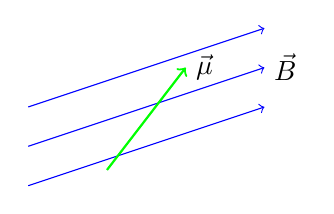
\begin{tikzpicture}[scale=1]
\draw[->,blue] (0,0) -- (3,1);
\draw[->,blue] (0,0.5) -- (3,1.5) node[right,black]{$\vec{B}$};
\draw[->,blue] (0,1) -- (3,2);
\draw[->,green,thick] (1,0.2) -- (2,1.5) node[right,black]{$\vec{\mu}$};

\end{tikzpicture}
\end{marginfigure}
But this interaction just turns the dipole so that it aligns with the magnetic field. Measuring the turning of a single atom is hard. It would be better if we could make this into a force. Then we could apply the force over some distance and measure the displacement or the change in kinetic energy. From classical physics, we know that $\vec{F}=-\vec{\nabla} V = \vec{\mu}\cdot(\vec{\nabla}\cdot\vec{B})$, so if we could make a magnetic field gradient, then the dipole would feel a force and we could measure this. We will model the magnetic field gradient as being only in a single direction (the $z$ direction). That means the force we are looking for is
\beq
\vec{F} = \mu_z \frac{\partial B_z}{\partial z}\hat{z}.
\eeq
\begin{marginfigure}\centering
\begin{tikzpicture}[scale=1]
\draw[->] (0,1,0) -- (.5,1,0) node[right]{$y$};
\draw[->] (0,1,0) -- (0,1.5,0) node[above]{$z$};
\draw[->] (0,1,0) -- (0,1,.5) node[left,below]{$x$};

%oven
\begin{scope}[canvas is zy plane at x=0]
\fill[black] (0,0,0) circle (.4) node[below,black,opacity=1,text width=1cm,align=center,shift={(-0.2,-0.6)}]{Atomic Beam Source};
\end{scope}

%atom beam
\fill[color=green!80,thick,decorate, decoration={shape backgrounds, shape=circle,shape size=0.2cm,shape sep={0.4cm, between centers}}](0,0,0) -- (5,0,0) ;

\draw[->,ultra thick,opacity=0.5](0,0,0) -- (0.65,0,0);

%field gradient zone
\begin{scope}[shift={(0,.15,0)}]
\begin{scope}[canvas is xz plane at y=.5,shift={(2,0,0)}]
\fill[blue,opacity=0.5] (-.5,-.5) rectangle +(1,1);
\end{scope}
\begin{scope}[canvas is yz plane at x=2.5]
\fill[blue,opacity=0.4] (-.5,-.5) rectangle +(1,1);
\end{scope}
\begin{scope}[canvas is xy plane at z=.5,shift={(2,0,0)}]
\fill[blue,opacity=0.3] (-.5,-.5) rectangle +(1,1);
\end{scope}
\end{scope}

%\draw[->,ultra thick] (2.5,0,0) -- (3.5,0,0);
\node[text width=2cm,align=center] at (2.0,-1.3,0) {$\partial B_z/ \partial z$ Gradient Zone};

\begin{scope}[canvas is yz plane at x=5]
\fill[orange,opacity=0.4] (-1,-1) rectangle +(2,2);
\end{scope}

\node[text width=2cm,align=center] at (4.5,-1.1,0) {Atom Position Detector};

\end{tikzpicture}
\end{marginfigure}
Practically, we make the magnetic field gradient using either a couple of strong permanent magnets or we can use a couple of current-carrying wires oriented so that there is a strong gradient between them. There are several ways of getting atoms into this field. The original Stern-Gerlach experiment used an atomic beam. More recent experiments use ultracold atoms. We follow the ideas of the Stern-Gerlach experiment for reasons that will make more sense later. In this experiment, the atoms feel the force in the magnetic field gradient zone, then travel in free space until the atoms reach a position detector that records their positions.

\begin{exercise}
Given a magnetic field gradient zone that is a fixed width and an atom position detector some distance away, find a formula that relates the magnetic dipole moment to the strength of the gradient and the relevant distances in the setup.

\end{exercise}

\begin{exercise}
One way to make a magnetic field gradient is to use two current-carrying wires in the anti-Helmholtz configuration (see \href{http://george.ph.utexas.edu/~meyrath/informal/electromagnets.pdf} {UTexas Electromagnet Design Basics
for Cold Atom Experiments, Equation 6}). What is the maximum field gradient to first-order if we use 3 amps of current with a radius of 10~cm?\marginnote{\texttt{george.ph.utexas.edu/ $\sim$meyrath/informal/ electromagnets.pdf}}

\end{exercise}

\subsection{Expected Result}
\begin{marginfigure}\centering
\begin{tikzpicture}[scale=1]
\draw[->] (0,1,0) -- (.5,1,0) node[right]{$y$};
\draw[->] (0,1,0) -- (0,1.5,0) node[above]{$z$};
\draw[->] (0,1,0) -- (0,1,.5) node[left,below]{$x$};

%oven
\begin{scope}[canvas is zy plane at x=0]
\fill[black] (0,0,0) circle (.4) node[below,black,opacity=1,text width=1cm,align=center,shift={(-0.2,-0.6)}]{Atomic Beam Source};
\end{scope}


%atom beam
\fill[color=green!80,thick,decorate, decoration={shape backgrounds, shape=circle,shape size=0.2cm,shape sep={0.4cm, between centers}}](0,0,0) -- (2,0,0) ;

\begin{scope}[shift={(2.4,0,0)}]
    \foreach \x in {-20,-15,...,20}
        \fill[color=magenta!80,thick,decorate, decoration={shape backgrounds, shape=circle,shape size=0.1cm,shape sep={0.4cm, between centers}}](0,0) -- (\x:2.6) ;
\end{scope}

\draw[->,ultra thick,opacity=0.5](0,0,0) -- (0.65,0,0);

%field gradient zone
\begin{scope}[shift={(0,.15,0)}]
\begin{scope}[canvas is xz plane at y=.5,shift={(2,0,0)}]
\fill[blue,opacity=0.5] (-.5,-.5) rectangle +(1,1);
\end{scope}
\begin{scope}[canvas is yz plane at x=2.5]
\fill[blue,opacity=0.4] (-.5,-.5) rectangle +(1,1);
\end{scope}
\begin{scope}[canvas is xy plane at z=.5,shift={(2,0,0)}]
\fill[blue,opacity=0.3] (-.5,-.5) rectangle +(1,1);
\end{scope}
\end{scope}

\draw[line width=0.1cm,magenta!80,line cap=round] (5,-0.9,0) -- (5,0.9,0);

\node[text width=2cm,align=center] at (2.0,-1.3,0) {$\partial B_z/ \partial z$ Gradient Zone};

\begin{scope}[canvas is yz plane at x=5]
\fill[orange,opacity=0.4] (-1,-1) rectangle +(2,2);
\end{scope}
%\node[text width=2cm,align=center] at (4.5,-1.1,0) {Atom Position Detector};

\end{tikzpicture}
\end{marginfigure}
The atoms enter the gradient zone with a randomly-oriented magnetic dipole moment. Since only the $z$-component of the dipole moment is affected by the gradient, we expect a shift in the atom's position on the detector based on the magnitude of $\mu_z$ which could be anything between ${-{}}\abs{\mu}$ and $\abs{\mu}$. This would give a continuous spread of detected positions.

\subsection{Actual Result}
\begin{marginfigure}\centering
\begin{tikzpicture}[scale=1]
\draw[->] (0,1,0) -- (.5,1,0) node[right]{$y$};
\draw[->] (0,1,0) -- (0,1.5,0) node[above]{$z$};
\draw[->] (0,1,0) -- (0,1,.5) node[left,below]{$x$};

%oven
\begin{scope}[canvas is zy plane at x=0]
\fill[black] (0,0,0) circle (.4) node[below,black,opacity=1,text width=1cm,align=center,shift={(-0.2,-0.6)}]{Atomic Beam Source};
\end{scope}


%atom beam
\fill[color=green!80,thick,decorate, decoration={shape backgrounds, shape=circle,shape size=0.2cm,shape sep={0.4cm, between centers}}](0,0,0) -- (2,0,0) ;

\begin{scope}[shift={(2.4,0,0)}]
\fill[color=green!80,thick,decorate, decoration={shape backgrounds, shape=circle,shape size=0.1cm,shape sep={0.4cm, between centers}}](0,0) -- (20:3.0);
\fill[color=green!80,thick,decorate, decoration={shape backgrounds, shape=circle,shape size=0.1cm,shape sep={0.4cm, between centers}}](0,0) -- (-20:3.0);
\end{scope}

\draw[->,ultra thick,opacity=0.5](0,0,0) -- (0.65,0,0);

%field gradient zone
\begin{scope}[shift={(0,.15,0)}]
\begin{scope}[canvas is xz plane at y=.5,shift={(2,0,0)}]
\fill[blue,opacity=0.5] (-.5,-.5) rectangle +(1,1);
\end{scope}
\begin{scope}[canvas is yz plane at x=2.5]
\fill[blue,opacity=0.4] (-.5,-.5) rectangle +(1,1);
\end{scope}
\begin{scope}[canvas is xy plane at z=.5,shift={(2,0,0)}]
\fill[blue,opacity=0.3] (-.5,-.5) rectangle +(1,1);
\end{scope}
\end{scope}

%\draw[line width=0.1cm,magenta!80,line cap=round] (5,-0.9,0) -- (5,0.9,0);

\node[text width=2cm,align=center] at (2.0,-1.3,0) {$\partial B_z/ \partial z$ Gradient Zone};

\begin{scope}[canvas is yz plane at x=5]
\fill[orange,opacity=0.4] (-1,-1) rectangle +(2,2);
\end{scope}
%\node[text width=2cm,align=center] at (4.5,-1.1,0) {Atom Position Detector};

\end{tikzpicture}
\end{marginfigure}
Perhaps it is not surprising (this is a quantum mechanic's course, after all), what actually happens is not this. What we measure is that the atoms either go all the way up or all the way down with 50\% probability for each direction. We calculate the magnetic dipole moment and get
\beq
\mu_z = \pm g \frac{e}{m_e}\frac{ \hbar}{2 }
\eeq
where $g$ is known as the Land\'{e} $g$-factor. \marginnote{For electrons, $g_e\approx2.00$, for protons, $g_p\approx5.58$ and for neutrons, $g_n\approx-3.82$.} This is an interesting result because $\hbar/2$ has units of angular momentum. We will split up the magnetic dipole moment into two pieces:
\beq
\vec{\mu} = \frac{q}{2m}\vec{S}
\label{eq:dipolespin}
\eeq
for an arbitrary charge $q$ and mass $m$. This new quantity which points in the same direction as the dipole moment has units of angular momentum and we call {\em spin}.\marginnote{Nothing, as far as we can tell, is actually spinning in a classical sense. We just call it that for historical reasons.} Our measurements of the magnetic dipole moment are thus measurements of the $z$-component of the spin vector. Since we get two values, they are either
\beq
S_z=\pm\frac{\hbar}{2}.
\eeq

\section{Rotated Spin Measurement}
\begin{marginfigure}\centering

\begin{tikzpicture}[scale=1]
\draw[->] (0,1,0) -- (.5,1,0) node[right]{$y$};
\draw[->] (0,1,0) -- (0,1.5,0) node[above]{$z$};
\draw[->] (0,1,0) -- (0,1,.5) node[left,below]{$x$};

%oven
\begin{scope}[canvas is zy plane at x=0]
\fill[black] (0,0,0) circle (.4) node[below,black,opacity=1,text width=1cm,align=center,shift={(-0.2,-0.6)}]{Atomic Beam Source};
\end{scope}


%atom beam
\fill[color=green!80,thick,decorate, decoration={shape backgrounds, shape=circle,shape size=0.2cm,shape sep={0.4cm, between centers}}](0,0,0) -- (2,0,0) ;

%\draw[line width=0.1cm,magenta!80,line cap=round] (5,-0.9,0) -- (5,0.9,0);

\node[text width=2cm,align=center] at (2.0,-1.3,0) {$\partial B_z/ \partial z$ Gradient Zone};

\pgfmathsetmacro{\rotangle}{-30}
\pgfmathsetmacro{\rotlen}{2.6}


\begin{scope}[canvas is yz plane at x=5]
\fill[orange,opacity=0.4] (-1,-1) rectangle +(2,2);
\draw[dashed] ({cos(\rotangle)*\rotlen*sin(20)},{-sin(\rotangle)*\rotlen*sin(20)}) -- ({-cos(\rotangle)*\rotlen*sin(20)},{sin(\rotangle)*\rotlen*sin(20)});
\end{scope}

\draw[->,ultra thick,opacity=0.5](0,0,0) -- (0.65,0,0);


\begin{scope}[shift={(2.4,0,0)}]
    \fill[color=green!80,thick,decorate, decoration={shape backgrounds, shape=circle,shape size=0.1cm,shape sep={0.4cm, between centers}}](0,0,0) -- ({\rotlen*cos(20)},{-\rotlen*sin(20)*cos(\rotangle)},{\rotlen*sin(20)*sin(\rotangle)});

    \fill[color=green!80,thick,decorate, decoration={shape backgrounds, shape=circle,shape size=0.1cm,shape sep={0.4cm, between centers}}](0,0,0) -- ({\rotlen*cos(20)},{\rotlen*sin(20)*cos(\rotangle)},{-\rotlen*sin(20)*sin(\rotangle)});
\end{scope}

    %field gradient zone

 \begin{scope}[shift={(0,.15,0)}]
 
    \begin{scope}[canvas is yz plane at x=2.5,rotate=-\rotangle]
    
    \fill[blue,opacity=0.4] (-.5,-.5) coordinate(A)--(-.5,.5)coordinate(B) -- (.5,.5) coordinate(C) -- (.5,-.5)coordinate(D)--cycle;
    \end{scope}
    \coordinate (E) at ($ (C) + (-1,0,0) $);
    \coordinate (F) at ($ (D) + (-1,0,0) $);
    \coordinate (G) at ($ (B) + (-1,0,0) $);
    \begin{scope}[shift={(2,0,0)}]
    \fill[blue,opacity=0.5] (C)-- (E)-- (F) -- (D) -- cycle;
    \fill[blue,opacity=0.3] (B)-- (G)-- (E) -- (C) -- cycle;
    \draw[->,thick] (A) -- (D);
    \end{scope}
 \node at (2.5,1.2,0) {$\hat{n}$};


 \end{scope}

%\node[text width=2cm,align=center] at (4.5,-1.1,0) {Atom Position Detector};

\end{tikzpicture}
\end{marginfigure}
Is the $z$-direction special because something happens to give the two results $S_z = \pm\hbar/2$? Perhaps gravity is doing something? We rotate the magnetic field gradient zone to check and we find that the two output atomic beams rotate with the gradient zone.
 
This looks exactly like our ElMaW experiments. No matter what direction we oriented the polarizer, we measured a probabilistic outcome of $\pm1$ with a 50\% probability of each outcome. So we use the same model to describe the quantum spin states. When the magnetic field gradient is pointed in the $z$-direction, we model the state of the atoms with the quantum states $\ket{u}$ and $\ket{d}$. We generalize this to the other possibilities for the direction of the magnetic field gradient, $\hat{n}$.\marginnote{This similarity is a deep connection. We call it $SU(2)$ symmetry and it is one of the core pieces of the Standard Model.}
\bas
\rmt{ If } \hat{n} =  \hat{z} & \rightarrow \begin{cases} \ket{u} & \rmt{measures }+ \frac{\hbar}{2}\\
\ket{d} & \rmt{measures } -\frac{\hbar}{2}
\end{cases}\\
\rmt{ If } \hat{n} =  \hat{x} & \rightarrow \begin{cases} \ket{r} & \rmt{measures } +\frac{\hbar}{2}\\
\ket{\ell} & \rmt{measures } -\frac{\hbar}{2}
\end{cases}\\
\rmt{ If } \hat{n} =  \hat{y} & \rightarrow \begin{cases} \ket{i} & \rmt{measures } +\frac{\hbar}{2}\\
\ket{o} & \rmt{measures } -\frac{\hbar}{2}
\end{cases}
\eas

\section{Changing Bases}
Just like we did with the ElMaW quantum state model, we can define the spin quantum states in one measurement direction in terms of the basis vectors in a different direction. We will begin with using the $z$-direction as our initial basis.

\begin{example}
What is the quantum state model if the input quantum spin is $\ket{\ell}$ or $\ket{r}$ spin and is measured in the $z$-basis?

\model We model the atomic spin as measured by the Stern-Gerlach experiment. We set the magnetic field gradient to $\hat{z}$ and measure in that basis. 

\vis We are looking at a system where someone give us either $\ket{\ell}$ or $\ket{r}$. They could prepare these using their own magnetic field gradient like the setup shown in Figure \ref{fig:spinexample13}.
\begin{figure}
\centering
\begin{tikzpicture}[scale=1]
\draw[->] (0,1,0) -- (.5,1,0) node[right]{$y$};
\draw[->] (0,1,0) -- (0,1.5,0) node[above]{$z$};
\draw[->] (0,1,0) -- (0,1,.5) node[left,below]{$x$};

%oven
\begin{scope}[canvas is zy plane at x=0]
\fill[black] (0,0,0) circle (.4) node[below,black,opacity=1,text width=1cm,align=center,shift={(-0.2,-0.6)}]{Atomic Beam Source};
\end{scope}


%atom beam
\fill[color=green!80,thick,decorate, decoration={shape backgrounds, shape=circle,shape size=0.3cm,shape sep={0.4cm, between centers}}](0,0,0) -- (2,0,0) ;

%\draw[line width=0.1cm,magenta!80,line cap=round] (5,-0.9,0) -- (5,0.9,0);


\pgfmathsetmacro{\rotangle}{-90}
\pgfmathsetmacro{\rotlen}{2.6}


\draw[->,ultra thick,opacity=0.5](0,0,0) -- (0.65,0,0);
    
\pgfmathsetmacro\bx{cos(\rotangle)*\rotlen}
\pgfmathsetmacro\by{sin(\rotangle)*\rotlen}

\begin{scope}[shift={(2.4,0,0)}]
    \fill[color=green!80,thick,decorate, decoration={shape backgrounds, shape=circle,shape size=0.15cm,shape sep={0.4cm, between centers}}](0,0,0) -- ({\rotlen*cos(20)},{-\rotlen*sin(20)*cos(\rotangle)},{\rotlen*sin(20)*sin(\rotangle)});

    \fill[color=green!80,thick,decorate, decoration={shape backgrounds, shape=circle,shape size=0.15cm,shape sep={0.4cm, between centers}}](0,0,0) -- ({\rotlen*cos(20)},{\rotlen*sin(20)*cos(\rotangle)},{-\rotlen*sin(20)*sin(\rotangle)});
\end{scope}

    %field gradient zone

 \begin{scope}[shift={(0,.15,0)}]
 
    \begin{scope}[canvas is yz plane at x=2.5,rotate=-\rotangle]
    
    \fill[blue,opacity=0.4] (-.5,-.5) coordinate(A)--(-.5,.5)coordinate(B) -- (.5,.5) coordinate(C) -- (.5,-.5)coordinate(D)--cycle;
    \end{scope}
    \coordinate (E) at ($ (C) + (-1,0,0) $);
    \coordinate (F) at ($ (D) + (-1,0,0) $);
    \coordinate (G) at ($ (B) + (-1,0,0) $);
    \coordinate (H) at ($ (A) + (-1,0,0) $);
    \begin{scope}[shift={(2,0,0)}]
    \fill[blue,opacity=0.5] (C)-- (E)-- (F) -- (D) -- cycle;
    \fill[blue,opacity=0.3] (A)-- (D)-- (F) -- (H) -- cycle;
    \draw[->,thick] (A) -- (D);
    \end{scope}
 \node at (2.5,1.2,0) {$\hat{x}$};


 \end{scope}

%\node[text width=2cm,align=center] at (4.5,-1.1,0) {Atom Position Detector};

%second gradient zone:
%field gradient zone
\begin{scope}[shift={({(\rotlen+0.5)*cos(20)},.15,{(\rotlen+0.5)*sin(20)})}]
\begin{scope}[canvas is xz plane at y=.5,shift={(2,0,0)}]
\fill[blue!50,opacity=1] (-.5,-.5) rectangle +(1,1);
\end{scope}
\begin{scope}[canvas is yz plane at x=2.5]
\fill[blue,opacity=0.4] (-.5,-.5) rectangle +(1,1);
\draw[->,thick] (-.5,-.5) -- (.5,-.5);
\end{scope}
\begin{scope}[canvas is xy plane at z=.5,shift={(2,0,0)}]
\fill[blue,opacity=0.3] (-.5,-.5) rectangle +(1,1);
\end{scope}
\end{scope}
 \node at (5.0,1,0) {$\hat{z}$};


\pgfmathsetmacro{\rotangle}{0}
%second atomic beams
\begin{scope}[shift={({2.4+(\rotlen+0.5)*cos(20)},0,{(\rotlen+0.5)*sin(20)})}]
    \fill[color=green!80,thick,decorate, decoration={shape backgrounds, shape=circle,shape size=0.075cm,shape sep={0.4cm, between centers}}](0,0,0) -- ({\rotlen*cos(20)},{-\rotlen*sin(20)*cos(\rotangle)},{\rotlen*sin(20)*sin(\rotangle)});

    \fill[color=green!80,thick,decorate, decoration={shape backgrounds, shape=circle,shape size=0.075cm,shape sep={0.4cm, between centers}}](0,0,0) -- ({\rotlen*cos(20)},{\rotlen*sin(20)*cos(\rotangle)},{-\rotlen*sin(20)*sin(\rotangle)});
\end{scope}

\begin{scope}[shift={({(\rotlen+0.5)*cos(20)},0,{(\rotlen+0.5)*sin(20)})}]
\begin{scope}[canvas is yz plane at x=5]
\fill[orange,opacity=0.4] (-1,-1) rectangle +(2,2);
\end{scope}
\end{scope}
\end{tikzpicture}
\caption[][2cm]{ }
\label{fig:spinexample13}
\end{figure}

\sol Using what we know from our quantum ElMaW model, we know that $\ket{\ell}$ must have an amplitude of $1/\stwo$ for each of $\ket{u}$ and $\ket{d}$ in order to give the 50\% measurement probability. So we'll try:
\beq
\ket{r} = \frac{1}{\stwo} \ket{u} + \frac{1}{\stwo} \ket{d}.
\eeq
If we then let $\ket{\ell} = \frac{1}{\stwo} \ket{u} - \frac{1}{\stwo} \ket{d}$, we have an orthonormal basis and that matches our model.


\assess The two states are orthogonal: $\avg{\ell|r}=0$ and they are both normalized. That is what we expect.

\end{example}

\begin{marginfigure}\centering
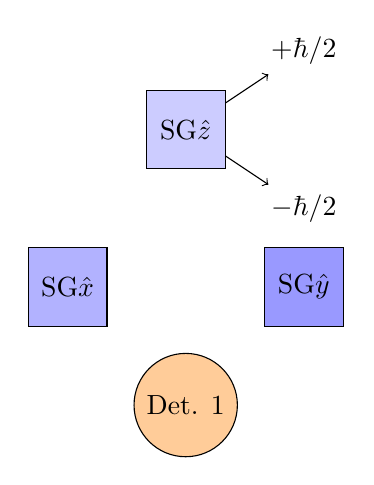
\begin{tikzpicture}
\node[fill=blue!20,shape=rectangle,draw,minimum size=1cm](z) at (0,2){SG$\hat{z}$};
\node (o1) at (1.5,3) {$+\hbar/2$};
\node (o2) at (1.5,1){$-\hbar/2$};
\draw[->] (z) -- (o1);
\draw[->] (z) -- (o2);
\node[fill=blue!30,shape=rectangle,draw,minimum size=1cm] at (-1.5,0){SG$\hat{x}$};
\node[fill=blue!40,shape=rectangle,draw,minimum size=1cm] at (1.5,0){SG$\hat{y}$};
\node[fill=orange!40,shape=circle,draw](D1) at (0,-1.5){Det. $1$};
\end{tikzpicture}
\end{marginfigure}
We can do this for the other two states, too \arnote{Go back to Section~\ref{sec:ybasis} and do this.}, writing $\ket{i}$ and $\ket{o}$ in terms of the $z$ basis vectors:
\bas
\ket{i} =& \frac{1}{\stwo}\ket{u} + \frac{\I}{\stwo}\ket{d}\\
\ket{o} =& \frac{1}{\stwo}\ket{u} - \frac{\I}{\stwo}\ket{d}.
\eas
For simplicity in drawing our experiments, we'll start drawing the magnetic field gradient zone as a simple box with the orientation of the field gradient on it. We use the shorthand ``SG'' to denote a Stern-Gerlach experiment. We can now link together multiple magnetic field gradient zones easily. We'll also label the detector as ``Det.'' We will model the upwards output as being the $+\hbar/2$ spin and the bottom as the $-\hbar/2$ output.

\begin{exercise}
\label{threeSGs}
Consider the following three experiments. You can simulate the outcome of the experiments using a Java \marginnote{I know Java has problems. Find a computer that will run the simulation. Ack.} simulator found at \href{http://www.physics.oregonstate.edu/~mcintyre/ph425/spins/index.html}{Oregon State's PHY425 Page.} Run the simulations and print the results. I want the total number of events and the fraction of events at each output port. \marginnote{\texttt{www.physics.oregonstate.edu/ $\sim$mcintyre/ph425/ spins/index.html}}

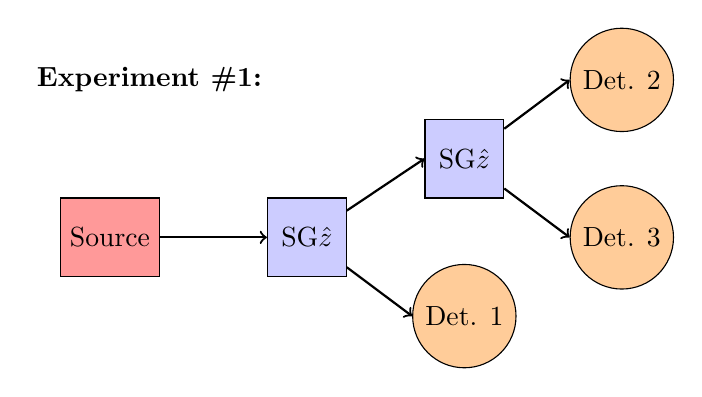
\begin{tikzpicture}
\node at (0,2) {\bf Experiment \#1:};
\node[fill=red!40,shape=rectangle,draw,minimum size=1cm](S) at (-0.5,0){Source};
\node[fill=blue!20,shape=rectangle,draw,minimum size=1cm](SG1) at (2,0){SG$\hat{z}$};
\draw[->,thick] (S) -- (SG1);
\node[fill=blue!20,shape=rectangle,draw,minimum size=1cm](SG2) at (4,1){SG$\hat{z}$};
\draw[->,thick] (SG1) -- (SG2.west);
\node[fill=orange!40,shape=circle,draw](D1) at (4,-1){Det. $1$};
\draw[->,thick] (SG1) -- (D1.west);
\node[fill=orange!40,shape=circle,draw](D2) at (6,2){Det. $2$};
\node[fill=orange!40,shape=circle,draw](D3) at (6,0){Det. $3$};
\draw[->,thick] (SG2) -- (D2.west);
\draw[->,thick] (SG2) -- (D3.west);
\end{tikzpicture}

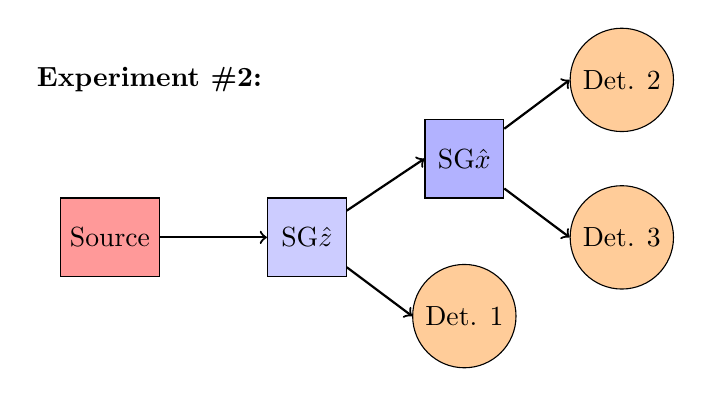
\begin{tikzpicture}
\node at (0,2) {\bf Experiment \#2:};
\node[fill=red!40,shape=rectangle,draw,minimum size=1cm](S) at (-0.5,0){Source};
\node[fill=blue!20,shape=rectangle,draw,minimum size=1cm](SG1) at (2,0){SG$\hat{z}$};
\draw[->,thick] (S) -- (SG1);
\node[fill=blue!30,shape=rectangle,draw,minimum size=1cm](SG2) at (4,1){SG$\hat{x}$};
\draw[->,thick] (SG1) -- (SG2.west);
\node[fill=orange!40,shape=circle,draw](D1) at (4,-1){Det. $1$};
\draw[->,thick] (SG1) -- (D1.west);
\node[fill=orange!40,shape=circle,draw](D2) at (6,2){Det. $2$};
\node[fill=orange!40,shape=circle,draw](D3) at (6,0){Det. $3$};
\draw[->,thick] (SG2) -- (D2.west);
\draw[->,thick] (SG2) -- (D3.west);
\end{tikzpicture}

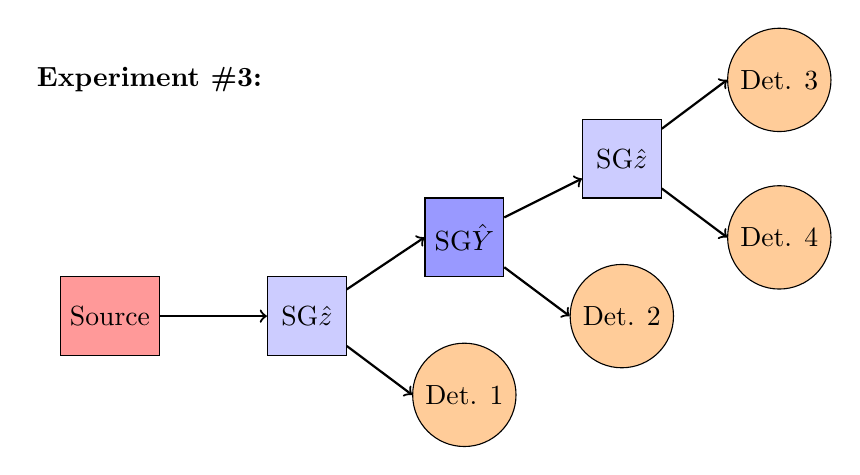
\begin{tikzpicture}
\node at (0,3) {\bf Experiment \#3:};
\node[fill=red!40,shape=rectangle,draw,minimum size=1cm](S) at (-0.5,0){Source};
\node[fill=blue!20,shape=rectangle,draw,minimum size=1cm](SG1) at (2,0){SG$\hat{z}$};
\draw[->,thick] (S) -- (SG1);

\node[fill=blue!40,shape=rectangle,draw,minimum size=1cm](SG2) at (4,1){SG$\hat{Y}$};
\draw[->,thick] (SG1) -- (SG2.west);
\node[fill=orange!40,shape=circle,draw](D1) at (4,-1){Det. $1$};
\draw[->,thick] (SG1) -- (D1.west);


\node[fill=blue!20,shape=rectangle,draw,minimum size=1cm](SG3) at (6,2){SG$\hat{z}$};
\draw[->,thick] (SG2) -- (SG3);
\node[fill=orange!40,shape=circle,draw](D2) at (6,0){Det. $2$};
\draw[->,thick] (SG2) -- (D2.west);

\node[fill=orange!40,shape=circle,draw](D3) at (8,3){Det. $3$};
\draw[->,thick] (SG3) -- (D3.west);
\node[fill=orange!40,shape=circle,draw](D4) at (8,1){Det. $4$};
\draw[->,thick] (SG3) -- (D4.west);
\end{tikzpicture}

\end{exercise}

\begin{example}
Design an ElMaW version of {\bf Experiment \#3} from Exercise \ref{threeSGs}. Sketch where you would need to put all of the optical components to make the equivalent quantum experiment.

\model We will model the ElMaW, beamsplitters, waveplates, and detectors as ideal. From what we've seen before, the spin $z$-basis maps to the ElMaW $V-H$ basis. So the spin $y$-basis must map to the $C_R-C_L$ basis for the ElMaW model.

\vis The layout for the ElMaW is shown in figure~\ref{fig:elmaw_ex3}.
\begin{figure}
\centering
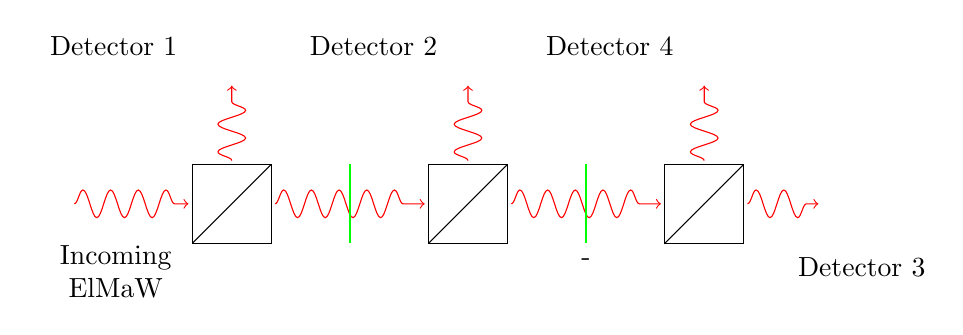
\begin{tikzpicture}


%incoming beam
\draw[red,->,decorate, decoration={snake,amplitude=5,segment length=10, post length=.1cm}](-2,0)--(-.55,0) node[midway, below,shift=({-.2cm,-.4cm}),text width=2cm,black,align=center]{Incoming ElMaW};

%PBS
\draw (-0.5,-.5) rectangle +(1,1);
\draw (-.5,-.5) -- (.5,.5);

%outgoing beam to 1
\draw[red,->,decorate, decoration={snake,amplitude=5,segment length=10, post length=.1cm}](.55,0)--(2.45,0);

\draw[red,->,decorate, decoration={snake,amplitude=5,segment length=10, post length=.1cm}](0,.55)--(0,1.50);
\detector{0.8}{0}{2.0}{90}
\node at (-1.5,2.0) {Detector 1};

\draw[thick,green] (1.5,.5) node[above,black] {\qwp} -- (1.5,-.5);

\draw (2.5,-.5) rectangle +(1,1);
\draw (2.5,-.5) -- (3.5,.5);
\draw[red,->,decorate, decoration={snake,amplitude=5,segment length=10, post length=.1cm}](3.55,0)--(5.45,0);
\draw[thick,green] (4.5,.5)  -- (4.5,-.5)node[below,black] {-\qwp};

\draw[red,->,decorate, decoration={snake,amplitude=5,segment length=10, post length=.1cm}](3,.55)--(3,1.50);
\detector{0.8}{3.8}{2.0}{90}
\node at (1.8,2.0) {Detector 2};

\draw (5.5,-.5) rectangle +(1,1);
\draw (5.5,-.5) -- (6.5,.5);
\draw[red,->,decorate, decoration={snake,amplitude=5,segment length=10, post length=.1cm}](6.55,0)--(7.45,0);

\detector{0.8}{9.4}{0}{0}
\node at (8,-.8) {Detector 3};

\draw[red,->,decorate, decoration={snake,amplitude=5,segment length=10, post length=.1cm}](6,.55)--(6,1.50);
\detector{0.8}{7.5}{2.0}{90}
\node at (4.8,2.0) {Detector 4};

\end{tikzpicture}
\caption[][2cm]{ }
\label{fig:elmaw_ex3}
\end{figure}

\end{example}

Although we have discussed how we measure the probability of getting a particular result (using the Eq.~(\ref{eq:prob})) \marginnote{\ref{tool:prob}}, we haven't addressed how to measure the spin state of our atoms. We need to add another set of tools to our toolbox in order to do this.

\section{The Bloch Sphere}



There is another way to represent the spin basis. The $x,y,z$ notation we have been using is similar to a 3-vector, so we will implement a graphical representation of the quantum state using a 3-vector called the {\em Bloch} vector. We map the quantum states onto a 3-dimensional space in the following way:
\begin{marginfigure}

\centering
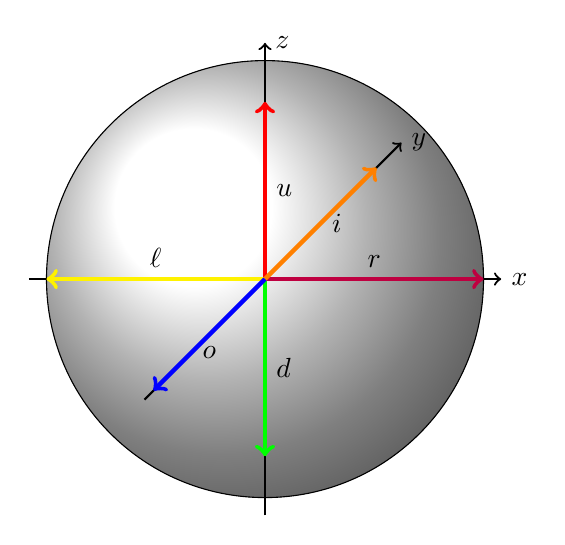
\begin{tikzpicture}[scale=0.75]

\def\R{3.7} % sphere radius
\def\angEl{35} % elevation angle
\filldraw[ball color=white] (0,0) circle (\R);
\foreach \t in {-80,-40,...,80} { \DrawLatitudeCircle[\R]{\t} }
\foreach \t in {-5,-55,...,-175} { \DrawLongitudeCircle[\R]{\t} }

\draw[->,thick](-4,0,0) -- (4,0,0)node[right]{$x$};
\draw[->,thick](0,-4,0) -- (0,4,0)node[right]{$z$};
\draw[->,thick](0,0,5.3) -- (0,0,-6)node[right]{$y$};

\draw[->,red,ultra thick](0,0,0)--(0,3,0) node[right,midway,black]{$\ket{u}$};
\draw[->,green,ultra thick](0,0,0)--(0,-3,0) node[right,midway,black]{$\ket{d}$};

\draw[->,purple,ultra thick](0,0,0)--(3.7,0,0) node[above,midway,black]{$\ket{r}$};
\draw[->,yellow,ultra thick](0,0,0)--(-3.7,0,0) node[above,midway,black]{$\ket{\ell}$};

\draw[->,orange,ultra thick](0,0,0)--(0,0,-4.9) node[right,midway,black]{$\ket{i}$};
\draw[->,blue,ultra thick](0,0,0)--(0,0,4.9) node[below,midway,black]{$\ket{o}$};

\end{tikzpicture}
\caption{The Bloch vector, represented as a unit vector on the Bloch sphere. }
\label{fig:blochsphere}
\end{marginfigure}%
\bas
\ket{u} & \rightarrow  +\hat{z} & \ket{r} & \rightarrow  +\hat{x}  & \ket{i} & \rightarrow  +\hat{y} \\
\ket{d} & \rightarrow  -\hat{z} & \ket{\ell} & \rightarrow  -\hat{x}  & \ket{o} & \rightarrow  -\hat{y} .
\eas
We represent this graphically using 3-vectors as shown in Figure~\ref{fig:blochsphere}. Do not confuse the representation of the quantum state as a Bloch vector with the 3-vectors. They behave in similar ways, but do not mean the same thing. For example, the length of the Bloch vector represents the total probability, so it will typically have a unit length. We can represent any arbitrary quantum state as a unit vector on the Bloch sphere. We have two free parameters to assign: we will use the polar angles $\theta$ (from the $\ket{u}$ vector) and $\phi$ (from the $\ket{r}$ vector), shown in Fig.~\ref{fig:blochangles}. An arbitrary quantum state is then written
\beq
\ket{A} = \cos{\frac{\theta}{2}}\ket{u} + \E{\I\phi} \sin{\frac{\theta}{2}}\ket{d}.
\eeq
\begin{marginfigure}
\centering
\begin{tikzpicture}[scale=1.3]
\draw[->,ultra thick,orange](0,0,0) -- (2,0,0)node[right,black]{$\ket{i}$};
\draw[->,ultra thick,red](0,0,0) -- (0,2,0)node[right,black]{$\ket{u}$};
\draw[->,ultra thick,purple](0,0,0) -- (0,0,2)node[right,black]{$\ket{r}$};
\draw[->,thick](0,0,0) -- (1.5,1,0.8)node[above]{$\ket{A}$};
\draw[dashed] (0,0,0) -- (1.5,0,.8);
\begin{scope}[rotate around={30:(0,0)}]
    \draw (0:0.5) arc (0:62:0.5)node[midway,above]{$\theta$};
\end{scope}

\begin{scope}[canvas is xz plane at y=0, rotate around={90:(0,0)}]
    \draw (0:0.5) arc (0:-62:0.5)node[midway,below]{$\phi$};
\end{scope}

\draw[dashed] (1.5,1,0.8) -- (1.5,0,.8);
\draw[dashed] (0,0,.8) -- (1.5,0,.8);
\draw[dashed] (1.5,0,0) -- (1.5,0,.8);
%\draw[dashed](1.5,1,.8) -- (2,1.33,1.1);
\end{tikzpicture}
\caption{Bloch angles}
\label{fig:blochangles}
\end{marginfigure}%
\begin{exercise}
Find the angles $\theta$ and $\phi$ needed to reproduce all three pairs of basis vectors for the quantum spin state.
\end{exercise}


\chapter{Quantum Operators}

We model the things we measure in our experiment with {\em linear operators}.\marginnote{These of often called ``observables'' because we could, in principle, observe them even if making the actual measurement is challenging.} We start with a general description of the operators and then we will apply them to our quantum state model.

\section{Linear Operators}
A linear operator is something of a machine that acts on quantum states and then returns quantum states:
\marginnote{We will use a ``hat'' $\hat{\;}$ on top of a capital letter ($\hat{M}$ for ``machine'') to denote a linear operator. This will keep it different from a unit vector.}
\beq
\hat{M}\ket{A} = \ket{B}.
\label{eq:linop}
\eeq
In order for our operator to be linear we want the following properties (where $z$ is a complex number):
\bas
\hat{M}z\ket{A} &= z\ket{B} \rmt{ and}\\
\hat{M}\left(\ket{A} + \ket{B}\right) &= \hat{M}\ket{A} + \hat{M}\ket{B}.
\eas

If we have a set of basis vectors like $\ket{j}$, we decompose our quantum states in terms of these vectors. We can then get what the operator $\hat{M}$ looks like in that particular basis. We start with\marginnote{Using \ref{tool:decom}}
\beq
\ket{A} = \sum_j \alpha_j\ket{j} \rmt{ and } \ket{B} = \sum_j \beta_j \ket{j}.
\eeq
We apply this to Eq.~(\ref{eq:linop}) to get
\beq
\sum_j \alpha_j \hat{M}\ket{j} = \sum_j \beta_j \ket{j}.
\eeq
We then multiply both sides by $\bra{k}$ and use the orthogonality relationship \marginnote{Our \ref{tool:orthog} tool} on the right-hand side to get
\beq
\sum_j \alpha_j \bra{k}\hat{M}\ket{j} = \beta_k.
\eeq
This means that, in the $\ket{j}$ basis, our operator is represented by 
\beq
\bra{k}\hat{M}\ket{j} \equiv m_{kj}\, ,
\label{eq:linopel}
\eeq
where we use the shorthand $m_{kj}$ to denote the elements of the $\hat{M}$ operator in this basis. So our linear operator represented in the $\ket{j}$ basis is
\beq
\sum_j m_{kj} \alpha_j = \beta_k,
\eeq
which looks a lot like matrix multiplication.


\subsection{Matrix Representation}
Just like we represented state vectors with column and row matrices, we form a representation of the operator using an $N$ by $N$ matrix, where $N$ is the number of free parameters in the state space. \marginnote{We also call $N$ the size of the Hilbert space. We will eventually find infinite-dimensional Hilbert spaces, but the same ideas apply.} So a matrix representation in a space with three free parameters would look like this:
\beq
\hat{M} \Meq
\begin{pmatrix} m_{11} & m_{12} & m_{13} \\
m_{21} & m_{22} & m_{23} \\
m_{31} & m_{32} & m_{33} \\
\end{pmatrix}.
\eeq
In this representation, our operator acting on our state vectors (Eq.~(\ref{eq:linop})) looks like this:
\beq
\begin{pmatrix} m_{11} & m_{12} & m_{13} \\
m_{21} & m_{22} & m_{23} \\
m_{31} & m_{32} & m_{33} \\
\end{pmatrix} 
\begin{pmatrix} \alpha_{1} \\
\alpha_{2} \\
\alpha_{3}\\
\end{pmatrix} = 
\begin{pmatrix} \beta_{1} \\
\beta_{2} \\
\beta_{3}\\
\end{pmatrix}
\eeq
\begin{example}
What is the outcome of the operator $\hat{M}$ acting on the state $\ket{A}$ in the $\ket{j}$ basis?

\model We model the operator and the quantum state vectors as matrices. We'll use matrix multiplication to get the output.

\vis Visualizing a matrix is tough. But one nice approach is the one by \href{http://people.cornellcollege.edu/dsherman/visualize-matrix.html}{Cornell College} where the matrix deforms the initial state into a new state. \marginnote{\texttt{people.cornellcollege.edu/dsherman/ visualize-matrix.html}}
\begin{figure}
\centering
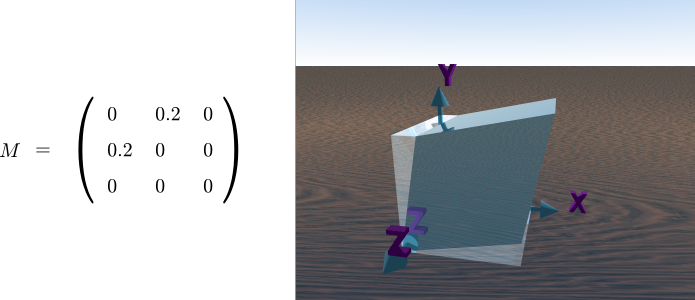
\includegraphics[width=8cm]{Mxy02yx02.png}
\end{figure}

\sol Our solution uses the rules of matrix multiplication to find the output.
\beq
\begin{pmatrix} m_{11} & m_{12} & m_{13} \\
m_{21} & m_{22} & m_{23} \\
m_{31} & m_{32} & m_{33} 
\end{pmatrix} 
\begin{pmatrix} \alpha_{1} \\
\alpha_{2} \\
\alpha_{3}
\end{pmatrix} = 
\begin{pmatrix} m_{11}\alpha_1+ m_{12}\alpha_2 +m_{13}\alpha_3  \\
m_{21}\alpha_1+ m_{22}\alpha_2 +m_{23}\alpha_3 \\
m_{31}\alpha_1+ m_{32}\alpha_2 +m_{33}\alpha_3
\end{pmatrix}.
\eeq

\assess Our output is a new ket vector as expected.

\end{example}

\section{Linear Operators acting on bra-vectors}

We need to know how linear operators act on bra vectors, too. We want something like
\beq
\bra{A}\hat{M}.
\eeq
So how are $\hat{M}\ket{A}=\ket{B}$ and $\bra{A}\hat{M}=\bra{B}$ related to each other? If we do this in component form (in the $\ket{j}$ basis), we get
\beq
\sum_j m_{kj} \alpha_j = \beta_k
\eeq
and
\beq
\sum_j m_{jk}^* \alpha_j^* = \beta_k^*.
\eeq
There are two differences between these two relationships:
\begin{enumerate}
\item We take the complex conjugate of each of the matrix entries.
\item We flip the location of the indices on each of the $m_{kj}$ entries. \marginnote{Also known as taking the transpose of the matrix.}
\end{enumerate}
Put these two together and we get the complex conjugate-transpose also known as the {\em Hermitian conjugate}. This is defined as
\beq
\left(\hat{M}^T\right)^* = \hat{M}^\dagger.
\eeq

\begin{exercise}
What is the Hermitian conjugate of this operator in the matrix representation?
\beq\hat{M}\Meq
\begin{pmatrix} \frac{1}{3} & 2+\I & \E{3\I\pi/2} \\
-4+2\I & \frac{2}{3} & 6 \\
\E{\I\pi/\sqrt{2}} & 9 & \frac{-1}{3}
\end{pmatrix} 
\eeq
\end{exercise}

\section{Operator Eigenvalues and Eigenvectors}
If a general linear operator transforms one ket vector into another ket vector, there is a special type of operator and related ket vector such that when the operator acts on the ket vector, it only scales the ket vector by some number. This special ket vector, known as the {\em eigenvector}, is otherwised unchanged. The scale factor is known as the {\em eigenvalue}. In symbolic terms we have\marginnote[-1cm]{This notation is awkward, but common. We have a ket vector in some basis $\ket{\lambda}$ and its eigenvalue $\lambda$ which is just a (complex) number.} 
\beq
\hat{L}\ket{\lambda} = \lambda\ket{\lambda}.
\label{eq:eigen}
\eeq\toolnote{\toollabel{tool:eigen}{\includegraphics{tool6.tikz} {\bf Eigenvaluator}}  This tool is used to evaluate the operation of a linear operator on one of its eigenvectors. It returns the eigenvalue and the eigenvector.} 
Let me give you a feel for how this works.
\begin{example}
Show that, in the matrix representation, $\ket{\lambda_1}\Meq\vket{1}{1}$ is an eigenvector of $\hat{M}\Meq\begin{pmatrix}1&2\\2&1\end{pmatrix}$.

\model It makes sense to use the matrix representation for our quantum states. We don't know much else about the system.

\vis This would be akin to multiplying a vector by some number or rotating a vector about is own axis. Hard to visualize.

\sol We run the operation $\hat{M}\ket{\lambda_1}$ and get $\vket{3}{3} \rightarrow 3 \ket{\lambda_1}$. That makes $\lambda_1=3$ and we have an eigenvalue and an eigenvector.\arnote{Work out this matrix multiplication in your notes.}

\assess We got a column vector from the operator acting on the column vector. That's what we expect.

\end{example}

\begin{exercise}
Check if $\vket{1}{0}$ and $\vket{1}{-1}$ are also eigenvectors of $\hat{M}\Meq\begin{pmatrix}1&2\\2&1\end{pmatrix}$. If they are, what are their eigenvalues?

\end{exercise}

\section{Hermitian Operators}
There is a special subset of linear operators that are equal to their own Hermitian conjugates:
\beq
\hat{M}^\dagger = \hat{M}.
\eeq%
We are particularly interested in this type of operator, called a {\em Hermitian Operator}, because of three properties:
\begin{enumerate}
\item The eigenvalues of a Hermitian operator are real numbers. This is good --- we will be identifying these as the outcomes of measurements and we only want real numbers for things we measure.
\item The eigenvectors of a Hermitian operator are a complete set. Any arbitrary ket-vector can be decomposed using our tools into the basis of eigenvectors.
\item The eigenvectors of a Hermitian operator can be made into an orthonormal set with unique eigenvalues. \marginnote[-1cm]{There are times when there are degenerate eigenvalues and a bit of work has to be done to get there, but we'll mostly be avoiding that situation in this Guide.}
\end{enumerate}

In the next example, we'll work through why it is that being a Hermitian operator means that the eigenvalues are real.
\begin{example}
Show that a Hermitian operator has real eigenvalues.

\model We model our quantum state as a ket-vector and our operator as Hermitian.

\vis Not much to show here--- but I'm thinking about it.

\sol Since $\hat{M}\ket{\lambda}=\lambda\ket{\lambda}$, we can flip this to the bra-vector version: $\bra{\lambda}\hat{M}^\dagger=\bra{\lambda}\lambda^*$. But since $\hat{M}^\dagger = \hat{M}$ (the definition of a Hermitian operator), that means that $\bra{\lambda}\hat{M}=\bra{\lambda}\lambda^*$.

Now we multiply the first piece by $\bra{\lambda}$ and the second by $\ket{\lambda}$ and get
\bas
\bra{\lambda}\hat{M}\ket{\lambda} &= \lambda\avg{\lambda|\lambda}\\
\bra{\lambda}\hat{M}\ket{\lambda} &= \lambda^*\avg{\lambda|\lambda}.
\eas
We subtract these two and get $\lambda - \lambda^*=0$ which is only valid if $\lambda$ is a real number.

\assess We got a general solution without having to use specific values.

\end{example}

\begin{exercise}
Show that if a Hermitian operator has two unique eigenvalues, the corresponding eigenvectors must be orthogonal.
\end{exercise}

\section{Spin Operators}
\label{sec:spinop}
\begin{marginfigure}\centering
\begin{tikzpicture}
\node[fill=blue!20,shape=rectangle,draw,minimum size=1cm](z) at (0,3){SG$\hat{z}$};
\node (o1) at (1.5,3) {$\hat{S}_z$};
\draw[->] (z) -- (o1);

\node[fill=blue!30,shape=rectangle,draw,minimum size=1cm](x) at (0,1.5){SG$\hat{x}$};
\node (o2) at (1.5,1.5) {$\hat{S}_x$};
\draw[->] (x) -- (o2);
\node[fill=blue!40,shape=rectangle,draw,minimum size=1cm](y) at (0,0){SG$\hat{y}$};
\node (o3) at (1.5,0) {$\hat{S}_y$};
\draw[->] (y) -- (o3);
\end{tikzpicture}
\end{marginfigure}


We wrap up this section by connecting Hermitian operators to our quantum spin model. We will now model the Stern-Gerlach magnetic field gradient as a Hermitian operator. Now the process of sending an atom through the magnetic field gradient becomes an operator acting on a quantum state. We will represent $\hat{S}_z$ as the matrix (in the $z$ basis)
\beq
\hat{S}_z \Meq \frac{\hbar}{2}\szmatrix .
\eeq
\begin{example}
What is the output state from the SG$\hat{z}$ if we sent in the state $\ket{u}$?

\model We model the SG magnetic field gradient as an operator in the $z$ basis. We will work in the matrix representation where $\ket{u} \Meq \vket{1}{0}$.

\vis 
\begin{figure}
\centering
\begin{tikzpicture}
\node(inputnd) at (-2,0){$\ket{u}$};
\node[fill=blue!20,shape=rectangle,draw,minimum size=1cm](zor) at (0,0){SG$\hat{z}$};
\draw[->] (inputnd) -- (zor);
\node (o1) at (1.5,1) {$+\hbar/2$};
\node (o2) at (1.5,-1){$-\hbar/2$};
\draw[->] (zor) -- (o1);
\draw[->] (zor) -- (o2);

\end{tikzpicture}
\end{figure}


\sol We want
\beq
\hat{S}_z\ket{u} \Meq \frac{\hbar}{2}\szmatrix\vket{1}{0}=\frac{\hbar}{2}\vket{1}{0}.
\eeq

So the output is the state $\hbar/2\ket{u}$. 

\assess This shows that $\ket{u}$ is an eigenvector of $\hat{S}_z$ as we expected with eigenvalue of $\hbar/2$.


\end{example}

We do the same thing with the other two directions, $x$ and $y$. We will write these operators in the same $z$ basis, though. That means when we want to use them, we have to write any input vector in the $z$-basis (in terms of $\ket{u}$ and $\ket{d}$).
\beq
\begin{split}
\hat{S}_z &\Meq \frac{\hbar}{2}\szmatrix\\
\hat{S}_x &\Meq \frac{\hbar}{2}\sxmatrix\\
\hat{S}_y &\Meq \frac{\hbar}{2}\symatrix 
\end{split}
\label{eq:sspins}
\eeq

\begin{exercise}
What is the output state if we send $\ket{\ell}$ into the $SG_x$ Stern-Gerlach experiment? How about if  $\ket{o}$ is sent into the $SG_y$?
\end{exercise}

\chapter{Quantum Mechanic's Model}

We now put everything together into a model to describe  both the ElMaW/Beamsplitter and the Stern-Gerlach experiments. 

\section{The Quantum Model}
Here's how the model works:
\begin{enumerate}
\item Measurable physical quantities are modeled as Hermitian operators $\hat{L}$ (where $\hat{L}^\dagger=\hat{L}$).
\item The results of a measurement is one of the eigenvalues of $\hat{L}$ called $\lambda_j$ where $\ket{\lambda_j}$ are the orthogonal eigenvectors of $\hat{L}$.
\item If we measure value $\lambda_j$, then the output state of the system is now $\ket{\lambda_j}$.
\item If $\ket{\Psi_\rmt{in}}$ is the state-vector input of a system, the probability of measuring value $\lambda_j$ is 
\beq
P(\lambda_j) = \abs{\avg{\lambda_j|\Psi_\rmt{in}}}^2 \mathnote{Using \ref{tool:prob}}. 
\eeq
\end{enumerate}



\section{Average Measurements}
\marginnote[-0.5cm]{Although this is often called an ``expectation value'', that is an awful name. There are many cases for which the most likely value and the average value are not the same.}
It is often useful to ask what we would get if we repeated a measurement many times and then took the average of all the results. We can evaluate this with our model using the following notation:\toolnote[0.2cm]{\toollabel{tool:avg}{\includegraphics{tool5.tikz} {\bf Expectation Evaluator}}  This tool is used to find the average measurement value of an operator for an input state.} 
\beq
\avg{\hat{L}} = \bra{\Psi_\rmt{in}}\hat{L}\ket{\Psi_\rmt{in}}.
\label{eq:avg}
\eeq
Let's practice using this tool.
\begin{example}
An atom is prepared in the spin state $\ket{\Psi}=\ket{u}.$ What is the average measurement if the atom is sent through the SG$\hat{z}$ magnetic field gradient?

\model We model the atom as a quantum state and the SG magnetic field gradient as the Hermitian operator $\hat{S}_z$. We will work in the $z$ basis where $\ket{u} \Meq\vket{1}{0}$.

\vis
\begin{figure}
\centering
\begin{tikzpicture}
\node(inputnd) at (-2,0){$\ket{u}$};
\node[fill=blue!20,shape=rectangle,draw,minimum size=1cm](zor) at (0,0){SG$\hat{z}$};
\draw[->] (inputnd) -- (zor);
\node (o1) at (1.5,1) {$+\hbar/2$};
\node (o2) at (1.5,-1){$-\hbar/2$};
\draw[->] (zor) -- (o1);
\draw[->] (zor) -- (o2);

\end{tikzpicture}
\end{figure}

\sol We use Eq.~(\ref{eq:avg}) \marginnote{\ref{tool:avg}} to calculate the average measurement. In the matrix representation, this becomes
\beq
\bra{u}\hat{S}_z\ket{u}\Meq \vbra{1}{0}\frac{\hbar}{2}\szmatrix\vket{1}{0}.
\eeq
Performing the matrix multiplication gives us $\hbar/2$. 

\assess That agrees with our experimental results. What is the probability of measuring $\ket{u}$? We find that $P(\ket{u}) = \abs{\avg{u|\Psi}}^2=1$.\marginnote{Using \ref{tool:prob}} After the measurement the state is still $\ket{u}$.

\end{example}

\begin{exercise}
An atom is prepared in the spin state $\ket{\Psi}=\ket{r}.$ 
\begin{enumerate}
\item What is the average measurement if the atom is sent through the SG$\hat{z}$ magnetic field gradient?
\item What is the probability of measuring $\hbar/2$ in a single experiment? 
\item What is the state after measurement if we measure $\hbar/2$?
\end{enumerate}
\end{exercise}

We model our ElMaW system using the same tools. We model the \hwp, \qwp, and PBS system using the following set of operators. If we write them all in the $V-H$ basis, we get:
\bas
(\lambda/2 = 0^\circ, \lambda/4=0^\circ )\equiv\hat{\sigma}_3&\Meq \szmatrix \\
(\lambda/2 = -45^\circ, \lambda/4=0^\circ ) \equiv\hat{\sigma}_1&\Meq \sxmatrix \\
(\lambda/2 = 0^\circ, \lambda/4=45^\circ )\equiv\hat{\sigma}_2&\Meq \symatrix .
\eas
The eigenvalues of each operator are the polarization states we've used before:
\bas
\hat{\sigma}_3\ket{V} & = +1 \ket{V}\mathnote{Using \ref{tool:eigen}}\\
\hat{\sigma}_3\ket{H} & = -1 \ket{H}.
\eas

We'll practice using this system, too.

\begin{example} 

We send the ElMaW from a single atom through a $V$ polarizer. What is the average measurement if the \hwp is set at ${-45}^\circ$?

\model We are given a state prepared in the $V-H$ basis, but since the \hwp is set at ${-45}^\circ$ and the \qwp is set at $0^\circ$, we need to measure in the $D_R-D_L$ basis. We will model the PBS in this basis and write our input state in that basis, too.

\vis 
\begin{figure}
\centering
\begin{tikzpicture}[scale=0.6]
\draw (-0.5,-.5) rectangle +(1,1) node[below,shift={(-.2,-.6)}]{PBS};
\draw (-.5,-.5) -- (.5,.5);
\draw[red,->,decorate, decoration={snake,amplitude=5,segment length=10, post length=.1cm}](-3.3,0)--(-.55,0) node[midway, above,shift=({0,.2cm})]{};
\draw[red,->,decorate, decoration={snake,amplitude=5,segment length=10, post length=.1cm}](.55,0)--(2,0);
\detector{1}{2.1}{0}{0}
\node at (2.5,-.8) {Detector 1};
\draw[red,->,decorate, decoration={snake,amplitude=5,segment length=10, post length=.1cm}](0,.55)--(0,2);
\detector{1}{0}{2.1}{90}
\node at (1.6,2.8) {Detector 2};
\fill[red] (-5,0) circle(0.1);
\draw[red,decorate,decoration={expanding waves,angle=35}](-5,0) -- (-3.5,0);
\draw[thick] (-3.5,.2) -- (-3.5,2);
\draw[thick] (-3.5,-.2) -- (-3.5,-2);
\draw[thick,green] (-2.5,-1) node[below,black,text width=1.5cm, align=left,shift={(.4,-.1)}] {\hwp at ${-45}^\circ$} -- (-2.5,1);
\draw[thick,blue] (-1.5,-1) -- (-1.5,1) node[above,shift={(-0.5,.3)},text width=2cm, align=right,black] {\qwp at $0^\circ$};
\end{tikzpicture}
\end{figure}

\sol We will use the eigenvalue relationships to find the average measurement. We need to write our initial state in the  $D_R-D_L$ basis:
\beq
\ket{\Psi} =\frac{1}{\stwo}\ket{D_R} + \frac{1}{\stwo}\ket{D_L}.\mathnote{\ref{tool:decom}}
\eeq
Now we want $\bra{\Psi}\hat{\sigma}_1\ket{\Psi}$. We do the right-hand part and get
\beq
\bra{\Psi}\left(\hat{\sigma}_1\ket{\Psi}\right) = \bra{\Psi}\hat{\sigma}_1\left(\frac{1}{\stwo}\ket{D_R} + \frac{1}{\stwo}\ket{D_L}\right)
\eeq
Now we use the eigenvalue relationships since $\ket{D_R}$ and $\ket{D_L}$ are both eigenvectors of $\hat{\sigma}_1$.
\beq
\bra{\Psi}\left(\hat{\sigma}_1\ket{\Psi}\right) = \bra{\Psi}\left((+1)\frac{1}{\stwo}\ket{D_R} + (-1)\frac{1}{\stwo}\ket{D_L}\right)\mathnote{\ref{tool:eigen}}
\eeq

Finally, we expand the bra-vector $\bra{\Psi}$ and use the fact that $\avg{D_R|D_L}=0$\marginnote{\ref{tool:orthog}} to get

\beq
\bra{\Psi}\hat{\sigma}_1\ket{\Psi}=\left((+1)\frac{1}{2} + (-1)\frac{1}{2}\right) = 0.
\eeq\arnote{Be sure to work out the missing steps here.}

\assess This is what we expected for our average measurement. Half the time we get a $+1$, the other half we get $-1$. This averages to zero.

\end{example}

\begin{exercise}
We send the ElMaW from a single atom through a $D_R$ polarizer.
\begin{enumerate}
\item What is the average measurement if the \hwp is set at $0^\circ$ and the \qwp is set at ${45}^\circ$?
\item What is the probability of measuring $-1$ in a single experiment? 
\item What is the state after measurement if we measure $-1$?
\end{enumerate}
\end{exercise}

\section{Averaging in a Specific Basis}
\label{sec:operatormodel4}
 \marginnote[-1cm]{Of course, we need to know the eigenvalues and eigenvectors of the operator to do this. You could use your favorite \CAS to find them for any operator in the matrix representation. \ref{tool:decom}} We can use our tools to figure out the average measurement of an operator $\hat{L}$ if we know we have decomposed the initial state vector $\ket{\Psi}$ in terms of its eigenvectors $\ket{\lambda_j}$.We start by writing 
\beq
\ket{\Psi} = \sum_j \alpha_j \ket{\lambda_j}. 
\eeq%
When we act on this state with the operator, we get
\beq
\hat{L}\ket{\Psi} = \sum_j\alpha_j \hat{L}\ket{\lambda_j} = \sum_j\alpha_j\lambda_j\ket{\lambda_j}.
\eeq%
So we now find the expectation value of $\avg{\hat{L}}$:
\bas
\bra{\Psi}\hat{L}\ket{\Psi} &= \sum_k \alpha_k^* \bra{\lambda_k}\sum_j \alpha_j \lambda_j \ket{\lambda_j}\\
\bra{\Psi}\hat{L}\ket{\Psi} &= \sum_k \alpha_k^* \alpha_k \lambda_k.
\eas\marginnote[-1cm]{\ref{tool:orthog}}%
We now relate this to the probability of making a measurement:
\beq
P(\lambda_j) = \abs{\avg{\lambda_j|\Psi}}^2 = \avg{\Psi|\lambda_j}\avg{\lambda_j|\Psi}\mathnote{\ref{tool:prob}}
\eeq
We now write our initial state in terms of the basis vectors $\ket{\lambda_k}$ and $\ket{\lambda_l}$:\marginnote{\ref{tool:decom}, \ref{tool:orthog}}
\bas
P(\lambda_j) =& \sum_k \alpha_k^* \avg{\lambda_k|\lambda_j} \sum_l \alpha_l \avg{\lambda_j|\lambda_l}\\
=& \alpha_j^* \alpha_j 
\eas%
This means that the average of many measurements can be written in the following compact way:\marginnote{This is the same as \ref{tool:avg} and joins that tool as another useful way of finding the expectation value.}
\beq
\bra{\Psi}\hat{L}\ket{\Psi} = \sum_j P(\lambda_j)\lambda_j.
\label{eq:probtoaverage}
\eeq
This agrees with the notion of an average measurement given a random distribution of outcomes.

\begin{tacticsbox}
\label{tec:expec}
Putting this all together, the general technique is to:
\begin{enumerate}
\item Model the physical system as a linear operator.
\item Determine the eigenvalues and eigenvectors of the operator.
\item Write the input state in the operator's eigenvector basis.
\item Calculate the average value of the measurement of the operator.
\end{enumerate}
\end{tacticsbox}

\begin{example}
What is the average measurement if a $C_R$ polarized wave is measured in the $V-H$ basis?

\model We model the ElMaW as a quantum state with initial state $\ket{C_R}$. We model the measurement system as a quantum operator $\hat{\sigma}_3$. Since we are working in the $V-H$ basis, we want to wite $\ket{C_R}$ in that basis.

\vis 
\begin{figure}
\centering
\begin{tikzpicture}[scale=0.6]
\draw (-0.5,-.5) rectangle +(1,1) node[below,shift={(-.2,-.6)}]{PBS};
\draw (-.5,-.5) -- (.5,.5);
\draw[red,->,decorate, decoration={snake,amplitude=5,segment length=10, post length=.1cm}](-3.3,0)--(-.55,0) node[midway, above,shift=({0,.2cm})]{};
\draw[red,->,decorate, decoration={snake,amplitude=5,segment length=10, post length=.1cm}](.55,0)--(2,0);
\detector{1}{2.1}{0}{0}
\node at (2.5,-.8) {Detector 1};
\draw[red,->,decorate, decoration={snake,amplitude=5,segment length=10, post length=.1cm}](0,.55)--(0,2);
\detector{1}{0}{2.1}{90}
\node at (1.6,2.8) {Detector 2};
\fill[red] (-5,0) circle(0.1);
\draw[red,decorate,decoration={expanding waves,angle=35}](-5,0) -- (-3.5,0);
\draw[thick] (-3.5,.2) -- (-3.5,2);
\draw[thick] (-3.5,-.2) -- (-3.5,-2);
\draw[thick,green] (-2.5,-1) node[below,black,text width=1.5cm, align=left,shift={(.4,-.1)}] {\hwp at $0^\circ$} -- (-2.5,1);
\draw[thick,blue] (-1.5,-1) -- (-1.5,1) node[above,shift={(-0.5,.3)},text width=2cm, align=right,black] {\qwp at $0^\circ$};
\end{tikzpicture}
\end{figure}

\sol We saw previously that $\ket{C_R} =  \frac{1}{\stwo}\ket{V} + \frac{\I}{\stwo}\ket{H}$. So 
\bas
P(+1) =& \abs{\frac{1}{\stwo}}^2  = \frac{1}{2}\\
P(-1) =& \abs{\frac{\I}{\stwo}}^2 = \frac{1}{2}
\eas

So our average measurement will be:
\beq
\bra{C_R}\hat{\sigma}_3\ket{C_R}= \frac{1}{2}(+1) + \frac{1}{2}(-1)=0.
\eeq \arnote{Be sure you know how we got here - work it out on your own.}

\assess This is what we expect should be - there are equal probabilities of measuring $\ket{V}$ and $\ket{H}$
\end{example}

\begin{exercise}
What is the average measurement if an atom has initial spin $\ket{\Psi}=(\sqrt{1/3})\ket{u} + (\sqrt{2/3})\ket{d}$ and is measured through the SG$\hat{y}$ magnetic field gradient?
\end{exercise}

\subsection{Common Misconception}
\begin{marginfigure}\centering
\begin{tikzpicture}[scale=0.6]
\draw (-0.5,-.5) rectangle +(1,1);
\draw (-.5,-.5) -- (.5,.5);
\draw[red,->,decorate, decoration={snake,amplitude=5,segment length=10, post length=.1cm}](-3.3,0)--(-.55,0) node[midway, above,shift=({0,.2cm})]{};
\draw[red,->,decorate, decoration={snake,amplitude=5,segment length=10, post length=.1cm}](.55,0)--(2,0);
\detector{1}{2.1}{0}{0}

\draw[red,->,decorate, decoration={snake,amplitude=5,segment length=10, post length=.1cm}](0,.55)--(0,2);
\detector{1}{0}{2.1}{90}
\draw[thick,green] (-2.5,-1) -- (-2.5,1);
\draw[thick,blue] (-1.5,-1) -- (-1.5,1) ;
\fill[black,opacity=0.3](-3,-1.2) rectangle (1.4,1.4) node[midway,below,black,opacity=1,shift={(0,-0.7)}]{Operator Model};


\begin{scope}[shift={(-3,-4)},scale=1.3]

%atom beam
\fill[color=green!80,thick,decorate, decoration={shape backgrounds, shape=circle,shape size=0.2cm,shape sep={0.4cm, between centers}}](0,0,0) -- (2.4,0,0) ;

\begin{scope}[shift={(2.4,0,0)}]
\fill[color=green!80,thick,decorate, decoration={shape backgrounds, shape=circle,shape size=0.1cm,shape sep={0.4cm, between centers}}](0,0) -- (20:3.0);
\fill[color=green!80,thick,decorate, decoration={shape backgrounds, shape=circle,shape size=0.1cm,shape sep={0.4cm, between centers}}](0,0) -- (-20:3.0);
\end{scope}

%field gradient zone
\begin{scope}[shift={(0,.15,0)}]
\begin{scope}[canvas is xz plane at y=.5,shift={(2,0,0)}]
\fill[blue,opacity=0.5] (-.5,-.5) rectangle +(1,1);
\end{scope}
\begin{scope}[canvas is yz plane at x=2.5]
\fill[blue,opacity=0.4] (-.5,-.5) rectangle +(1,1);

\end{scope}
\begin{scope}[canvas is xy plane at z=.5,shift={(2,0,0)}]
\fill[blue,opacity=0.3] (-.5,-.5) rectangle +(1,1);

\end{scope}

\draw[->,thick](2.5,-.5,-.5)--(2.5,.5,-.5);

\end{scope}


\begin{scope}[canvas is yz plane at x=5]
\fill[orange,opacity=0.4] (-1,-1) rectangle +(2,2);
\end{scope}
%\node[text width=2cm,align=center] at (4.5,-1.1,0) {Atom Position Detector};

\fill[black,opacity=0.3](1,-1) rectangle (3,1)node[midway,below,black,opacity=1,shift={(0,-0.7)}]{Operator Model};


\end{scope}

\end{tikzpicture}
\end{marginfigure}
It is a common misconception that acting with an operator is the same thing as making a measurement with an actual physical system. That isn't how our model works. We can use the operator model to figure out what the {\em average} of many measurements will be. We can use the probability tool to figure out what the probability of any particular measurement will be. We can even say what the measurement value will be and what the resulting state is if we make a particular measurement. But the operator does not model a measurement. It models the interaction system {\em prior to} the measurement devices. We will say more about how to model the actual measurement devices a bit later on.


\section{Non-uniqueness of the Quantum State}
We have addressed this before, but I want to make sure we have hit this concept explicitly. The quantum state is only specified up to an arbitbitrary phase factor $\E{\I \theta}$. This is because all of our normalizations and measurements are based on taking the state vector times its complex conjugate. So if
\beq
\ket{\Psi} = \E{\I\theta}\ket{A},
\eeq
then 
\beq
\avg{\Psi|\Psi} = \bra{A}\E{-\I\theta}\E{\I\theta}\ket{A} = \avg{A|A}.
\eeq
So the phase factor $\theta$ could be anything at all and it won't affect the outcome of the measurement. This can be handy as it will allow us to ignore any overall phases.\marginnote[-3cm]{This is similar to the idea from classical physics that only energy differences matter and not absolute energies. This arbitrary phase factor plays an important role in developing ideas beyond this class.}

\begin{exercise}
You are given a beam of atoms that are all prepared in the intial state
\beq
\ket{\Psi} = \frac{1}{2} \ket{u} + \frac{\sqrt{3}\I}{2}\ket{d}.
\eeq
You are also given a new system that is modeled by the following Hermitian operator:
\beq
\hat{B} = b_0\begin{pmatrix}1&1\\1&1\end{pmatrix}
\eeq
where $b_0$ is a real constant. 
\begin{enumerate}
\item What are the possible outcomes of the measurements? What are the probabilities of getting each?
\item If we make many measurements with this system, what is the average value of the measurements? Calculate this two different ways: using the probabilities from the first part, and using the definition of the average of an operator.
\end{enumerate}

\end{exercise}


\chapter{Part \ref{part1} Summary and Test}

Up to this point we have covered the need for a quantum model to describe two different experiment systems: the ElMaWs from a single trapped atom and the internal spin states of atoms. We developed a mathematical model for describing measurement probabilities and outcomes based on a complex vector space. We developed a set of tools that we used to make specific predictions of the average outcomes of measurements of these systems.

It is important to practice using these tools to model experiments. The following set of exercises is a good way to test your understanding of these models. Try to do these without referring to the previous text. If you can do all of them and your solutions agree with those provided on the following pages, then you are in pretty good shape to move forward with the material. If not, you should specifically review the material  you do not have mastery of yet, then retry the test exercises.

\begin{exercise}
Your research advisor asks you to produce a beam of spin-$1/2$ atoms which are in the state
\beq
\ket{\Psi} = -\frac{1}{\stwo}\ket{u} + \frac{\I}{\stwo}\ket{d}.
\eeq
\begin{enumerate}
\item You measure the state using a Stern-Gerlach apparatus oriented in the $y$-direction. What is the probability of getting a ${-\hbar/2}$ result?
\item What is the state of the atoms after you measure a ${-\hbar/2}$ result?
\item What is the expected average if you prepare many atoms in the same state and then measure them?
\end{enumerate}
\end{exercise}

\begin{exercise}
Consider two measurement propositions about a atomic spin state initially prepared as $\ket{\ell}$:
\begin{enumerate}
\item[Prop. A:] When measured with an SG$\hat{x}$, do we measure ${-\hbar/2}$?
\item[Prop. B:] When measured with an SG$\hat{z}$, do we measure ${-\hbar/2}$?
\end{enumerate}
For which measurement results will these propositions be true? How about A {\bf and} B as well as A {\bf or} B? Consider the reverse as well: B {\bf and} A and B {\bf or} A.
\end{exercise}

\begin{exercise}
Identify the nature (bra, ket, operator, or number) of the following: 
\begin{enumerate}
\item $\avg{\psi|\phi}\hat{A}$
\item $\hat{A}\ket{\psi}\avg{\phi|\psi}$
\item $\hat{B}\ket{\psi}\bra{\phi}\hat{A}\ket{\psi} $ 
\end{enumerate}

Why must the bra and ket  vectors we use be normalized to one?
\end{exercise}

\begin{exercise}
You are given a beam of atoms that are all prepared in the intial state
\beq
\ket{\Psi} = \frac{-2}{\sqrt{7}} \ket{u} + \I \sqrt{\frac{3}{7}}\ket{d}.
\eeq
You are also given a new system that is modeled by the following operator in the $z$-basis:
\beq
\hat{W} \Meq 2\begin{pmatrix}9&0\\0&16\end{pmatrix}
\eeq
\begin{enumerate}
\item Show that $\hat{W}$ is a Hermitian operator. What are the eigenvalues and eigenvectors of the operator.
\item What is the average measurement of $\avg{\hat{W}}$ for the given input state $\ket{\Psi}$?
\end{enumerate}

\end{exercise}

Stop here and don't continue reading until you have completed the exercises.
\newpage
\begin{example}
We model the atom as a quantum state and we model the measurement as the operator $\hat{S}_y$. We first notice that the input state $\ket{\Psi} = -\ket{o}$. This simplifies the problem significantly, since $\ket{o}$ is an eigenvector of the $\hat{S}_y$ operator.

\begin{enumerate}
\item The probability of measuring ${-\hbar}/2$ is just the probability of measuring $\ket{o}$. Since the input state is $\ket{\Psi} = -\ket{o}$, the probability is
\beq
P(\ket{o}) = \abs{\avg{o|\Psi}}^2 = \abs{-1}^2 = 1.
\eeq
\item After measuring ${-\hbar}/2$, the atom is in the state $\ket{o}$, since that is the eignevector of $\hat{S}_y$ with eigenvalue of ${-\hbar}/2$.
\item The average result after making many measurements is just ${-\hbar}/2$, since the probability of making this measurement is $1$.
\end{enumerate}
\end{example}

\begin{example}
We model the two measurements as the quantum operators $\hat{S}_x$ and $\hat{S}_z$. The output of the measurements are:
\bas
\hat{S}_x\ket{\ell} =& \frac{-\hbar}{2}\ket{\ell}\\
\hat{S}_z\ket{\ell} =& \hat{S}_z\left(\frac{1}{\stwo}\ket{u}-\frac{1}{\stwo}\ket{d}\right) = \frac{\hbar}{2}\frac{1}{\stwo}\ket{u} - \left(\frac{-\hbar}{2}\right)\frac{1}{\stwo}\ket{d}.
\eas
Prop. A is true 100\% of the time.
Prop. B is true 50\% of the time since the probability of measuring ${-\hbar}/2$ is 50\%.
The proposition {\bf A or B} is always true since the probability of measuring A is 100\%. The proposition {\bf A and B} can be visualized using our schematic diagram shown in Fig.~\ref{fig:t1}.
\begin{figure}
\centering
\begin{tikzpicture}
\node(inputnd) at (-2,0){$\ket{\ell}$};
\node[fill=blue!20,shape=rectangle,draw,minimum size=1cm](xor) at (0,0){SG$\hat{x}$};
\draw[->] (inputnd) -- (zor);
\node (o1) at (2,1) {$+\hbar/2$ -- 0\% of the time.};
\node[fill=blue!20,shape=rectangle,draw,minimum size=1cm](zor) at (2,-1){SG$\hat{z}$};
\node[text width=2cm] (o2) at (4,-2){$-\hbar/2$ True 50\% of the time.};
\node[text width=2cm] (o3) at (4,0){$+\hbar/2$ False};
\draw[->](xor) -- (o1);
\draw[->](xor) -- (zor) node[below,midway]{True};
\draw[->] (zor) -- (o3);
\draw[->] (zor) -- (o2);
\end{tikzpicture}
\caption[][2cm]{ }
\label{fig:t1}
\end{figure}

So the proposition {\bf A and B} is true 50\% of the time.

We reverse this to look at the other propositions, shown in Fig.~\ref{fig:t2}. This shows that the proposition is true 25\% of the time.
\begin{figure}
\centering
\begin{tikzpicture}
\node(inputnd) at (-2,0){$\ket{\ell}$};
\node[fill=blue!20,shape=rectangle,draw,minimum size=1cm](xor) at (0,0){SG$\hat{z}$};
\draw[->] (inputnd) -- (xor);
\node (o1) at (1.5,1) {$+\hbar/2$ -- 50\% of the time.};
\node[fill=blue!20,shape=rectangle,draw,minimum size=1cm](zor) at (2,-1){SG$\hat{x}$};
\node[text width=2cm] (o2) at (4,-2){$-\hbar/2$ True 50\% of the time.};
\node (o3) at (4,0){$+\hbar/2$ -- False};
\draw[->](xor) -- (o1);
\draw[->](xor) -- (zor) node[below,midway,text width=1cm]{True 50\% of the time};
\draw[->] (zor) -- (o3);
\draw[->] (zor) -- (o2);
\end{tikzpicture}
\caption[][2cm]{ }
\label{fig:t2}
\end{figure}

Finally we look at the proposition {\bf B or A}. This is shown in Fig.~\ref{fig:t3}. The total possibility of getting a true result is 75\%.
\begin{figure}
\centering
\begin{tikzpicture}
\node(inputnd) at (-2,0){$\ket{\ell}$};
\node[fill=blue!20,shape=rectangle,draw,minimum size=1cm](xor) at (0,0){SG$\hat{z}$};
\draw[->] (inputnd) -- (xor);
\node (o1) at (2,-1) {$-\hbar/2$ -- True 50\% of the time.};
\node[fill=blue!20,shape=rectangle,draw,minimum size=1cm](zor) at (2,1){SG$\hat{x}$};
\node(o2) at (4,0){$-\hbar/2$ True 50\% of the time.};
\node (o3) at (4,2){$+\hbar/2$ -- False};
\draw[->](xor) -- (o1);
\draw[->](xor) -- (zor);
\draw[->] (zor) -- (o3);
\draw[->] (zor) -- (o2);
\end{tikzpicture}
\caption[][2cm]{ }
\label{fig:t3}
\end{figure}
\end{example}

\begin{example}
We identify the items as:
\begin{enumerate}
\item This is a number times an operator which gives an operator.
\item This is a ket times a number which give a ket.
\item Thi is a ket times a number which gives a ket.
\end{enumerate}
The states must be normalized because we identify the norm as the total measurement probability. Because we must measure the system in some state with 100\% probability, the norm of the state better be $1$.

\end{example}

\begin{example}
We first look at the operator $\hat{W}$. Its Hermitian conjugate $\hat{W}^\dagger$ is 
\beq
\hat{W}^\dagger \Meq 2\begin{pmatrix}9&0\\0&16\end{pmatrix} = \hat{W},
\eeq
so the operator is Hermitian. We also notice that it is diagonal. This means that the eigenvectors are just $\ket{u}$ and $\ket{d}$. The two eigenvalues are:
\beq
\hat{W}\ket{u} = 18 \ket{u} \qquad \hat{W}\ket{d} = 32\ket{d}.
\eeq\marginnote[-1cm]{This is a ``Wabash'' operator: it has eignevalues 1832!}

The average measurement is
\beq
\avg{\hat{W}} = P(\ket{u})(18) + P(\ket{d})(32) = \frac{4}{7}(18) + \frac{3}{7}(32) = 24.
\eeq

\end{example}


%sagemathcloud={"latex_command":""}